\documentclass[twoside]{book}

% Packages required by doxygen
\usepackage{fixltx2e}
\usepackage{calc}
\usepackage{doxygen}
\usepackage[export]{adjustbox} % also loads graphicx
\usepackage{graphicx}
\usepackage[utf8]{inputenc}
\usepackage{makeidx}
\usepackage{multicol}
\usepackage{multirow}
\PassOptionsToPackage{warn}{textcomp}
\usepackage{textcomp}
\usepackage[nointegrals]{wasysym}
\usepackage[table]{xcolor}

% Font selection
\usepackage[T1]{fontenc}
\usepackage[scaled=.90]{helvet}
\usepackage{courier}
\usepackage{amssymb}
\usepackage{sectsty}
\renewcommand{\familydefault}{\sfdefault}
\allsectionsfont{%
  \fontseries{bc}\selectfont%
  \color{darkgray}%
}
\renewcommand{\DoxyLabelFont}{%
  \fontseries{bc}\selectfont%
  \color{darkgray}%
}
\newcommand{\+}{\discretionary{\mbox{\scriptsize$\hookleftarrow$}}{}{}}

% Page & text layout
\usepackage{geometry}
\geometry{%
  a4paper,%
  top=2.5cm,%
  bottom=2.5cm,%
  left=2.5cm,%
  right=2.5cm%
}
\tolerance=750
\hfuzz=15pt
\hbadness=750
\setlength{\emergencystretch}{15pt}
\setlength{\parindent}{0cm}
\setlength{\parskip}{3ex plus 2ex minus 2ex}
\makeatletter
\renewcommand{\paragraph}{%
  \@startsection{paragraph}{4}{0ex}{-1.0ex}{1.0ex}{%
    \normalfont\normalsize\bfseries\SS@parafont%
  }%
}
\renewcommand{\subparagraph}{%
  \@startsection{subparagraph}{5}{0ex}{-1.0ex}{1.0ex}{%
    \normalfont\normalsize\bfseries\SS@subparafont%
  }%
}
\makeatother

% Headers & footers
\usepackage{fancyhdr}
\pagestyle{fancyplain}
\fancyhead[LE]{\fancyplain{}{\bfseries\thepage}}
\fancyhead[CE]{\fancyplain{}{}}
\fancyhead[RE]{\fancyplain{}{\bfseries\leftmark}}
\fancyhead[LO]{\fancyplain{}{\bfseries\rightmark}}
\fancyhead[CO]{\fancyplain{}{}}
\fancyhead[RO]{\fancyplain{}{\bfseries\thepage}}
\fancyfoot[LE]{\fancyplain{}{}}
\fancyfoot[CE]{\fancyplain{}{}}
\fancyfoot[RE]{\fancyplain{}{\bfseries\scriptsize Generated by Doxygen }}
\fancyfoot[LO]{\fancyplain{}{\bfseries\scriptsize Generated by Doxygen }}
\fancyfoot[CO]{\fancyplain{}{}}
\fancyfoot[RO]{\fancyplain{}{}}
\renewcommand{\footrulewidth}{0.4pt}
\renewcommand{\chaptermark}[1]{%
  \markboth{#1}{}%
}
\renewcommand{\sectionmark}[1]{%
  \markright{\thesection\ #1}%
}

% Indices & bibliography
\usepackage{natbib}
\usepackage[titles]{tocloft}
\setcounter{tocdepth}{3}
\setcounter{secnumdepth}{5}
\makeindex

% Hyperlinks (required, but should be loaded last)
\usepackage{ifpdf}
\ifpdf
  \usepackage[pdftex,pagebackref=true]{hyperref}
\else
  \usepackage[ps2pdf,pagebackref=true]{hyperref}
\fi
\hypersetup{%
  colorlinks=true,%
  linkcolor=blue,%
  citecolor=blue,%
  unicode%
}

% Custom commands
\newcommand{\clearemptydoublepage}{%
  \newpage{\pagestyle{empty}\cleardoublepage}%
}

\usepackage{caption}
\captionsetup{labelsep=space,justification=centering,font={bf},singlelinecheck=off,skip=4pt,position=top}

%===== C O N T E N T S =====

\begin{document}

% Titlepage & ToC
\hypersetup{pageanchor=false,
             bookmarksnumbered=true,
             pdfencoding=unicode
            }
\pagenumbering{roman}
\begin{titlepage}
\vspace*{7cm}
\begin{center}%
{\Large Heat conduction equation }\\
\vspace*{1cm}
{\large Generated by Doxygen 1.8.11}\\
\end{center}
\end{titlepage}
\clearemptydoublepage
\tableofcontents
\clearemptydoublepage
\pagenumbering{arabic}
\hypersetup{pageanchor=true}

%--- Begin generated contents ---
\chapter{Hierarchical Index}
\section{Class Hierarchy}
This inheritance list is sorted roughly, but not completely, alphabetically\+:\begin{DoxyCompactList}
\item \contentsline{section}{I\+O\+Manager}{\pageref{classIOManager}}{}
\item \contentsline{section}{Method}{\pageref{classMethod}}{}
\begin{DoxyCompactList}
\item \contentsline{section}{Analytical}{\pageref{classAnalytical}}{}
\item \contentsline{section}{Explicit}{\pageref{classExplicit}}{}
\begin{DoxyCompactList}
\item \contentsline{section}{Dufort\+Frankel}{\pageref{classDufortFrankel}}{}
\item \contentsline{section}{F\+T\+CS}{\pageref{classFTCS}}{}
\item \contentsline{section}{Richardson}{\pageref{classRichardson}}{}
\end{DoxyCompactList}
\item \contentsline{section}{Implicit}{\pageref{classImplicit}}{}
\begin{DoxyCompactList}
\item \contentsline{section}{Crank\+Nicolson}{\pageref{classCrankNicolson}}{}
\item \contentsline{section}{Laasonen}{\pageref{classLaasonen}}{}
\end{DoxyCompactList}
\end{DoxyCompactList}
\item \contentsline{section}{Problem}{\pageref{classProblem}}{}
\item vector\begin{DoxyCompactList}
\item \contentsline{section}{Matrix}{\pageref{classMatrix}}{}
\item \contentsline{section}{Vector}{\pageref{classVector}}{}
\end{DoxyCompactList}
\end{DoxyCompactList}

\chapter{Class Index}
\section{Class List}
Here are the classes, structs, unions and interfaces with brief descriptions\+:\begin{DoxyCompactList}
\item\contentsline{section}{\hyperlink{classAnalytical}{Analytical} }{\pageref{classAnalytical}}{}
\item\contentsline{section}{\hyperlink{classCrankNicolson}{Crank\+Nicolson} }{\pageref{classCrankNicolson}}{}
\item\contentsline{section}{\hyperlink{classDufortFrankel}{Dufort\+Frankel} }{\pageref{classDufortFrankel}}{}
\item\contentsline{section}{\hyperlink{classExplicit}{Explicit} }{\pageref{classExplicit}}{}
\item\contentsline{section}{\hyperlink{classFTCS}{F\+T\+CS} }{\pageref{classFTCS}}{}
\item\contentsline{section}{\hyperlink{classImplicit}{Implicit} }{\pageref{classImplicit}}{}
\item\contentsline{section}{\hyperlink{classIOManager}{I\+O\+Manager} }{\pageref{classIOManager}}{}
\item\contentsline{section}{\hyperlink{classLaasonen}{Laasonen} }{\pageref{classLaasonen}}{}
\item\contentsline{section}{\hyperlink{classMatrix}{Matrix} }{\pageref{classMatrix}}{}
\item\contentsline{section}{\hyperlink{classMethod}{Method} }{\pageref{classMethod}}{}
\item\contentsline{section}{\hyperlink{classProblem}{Problem} }{\pageref{classProblem}}{}
\item\contentsline{section}{\hyperlink{classRichardson}{Richardson} }{\pageref{classRichardson}}{}
\item\contentsline{section}{\hyperlink{classVector}{Vector} }{\pageref{classVector}}{}
\end{DoxyCompactList}

\chapter{File Index}
\section{File List}
Here is a list of all files with brief descriptions\+:\begin{DoxyCompactList}
\item\contentsline{section}{\hyperlink{main_8cpp}{main.\+cpp} }{\pageref{main_8cpp}}{}
\item\contentsline{section}{grid/\hyperlink{matrix_8cpp}{matrix.\+cpp} }{\pageref{matrix_8cpp}}{}
\item\contentsline{section}{grid/\hyperlink{matrix_8h}{matrix.\+h} }{\pageref{matrix_8h}}{}
\item\contentsline{section}{grid/\hyperlink{vector_8cpp}{vector.\+cpp} }{\pageref{vector_8cpp}}{}
\item\contentsline{section}{grid/\hyperlink{vector_8h}{vector.\+h} }{\pageref{vector_8h}}{}
\item\contentsline{section}{io/\hyperlink{iomanager_8cpp}{iomanager.\+cpp} }{\pageref{iomanager_8cpp}}{}
\item\contentsline{section}{io/\hyperlink{iomanager_8h}{iomanager.\+h} }{\pageref{iomanager_8h}}{}
\item\contentsline{section}{methods/\hyperlink{analytical_8cpp}{analytical.\+cpp} }{\pageref{analytical_8cpp}}{}
\item\contentsline{section}{methods/\hyperlink{analytical_8h}{analytical.\+h} }{\pageref{analytical_8h}}{}
\item\contentsline{section}{methods/\hyperlink{method_8cpp}{method.\+cpp} }{\pageref{method_8cpp}}{}
\item\contentsline{section}{methods/\hyperlink{method_8h}{method.\+h} }{\pageref{method_8h}}{}
\item\contentsline{section}{methods/explicit/\hyperlink{dufort__frankel_8cpp}{dufort\+\_\+frankel.\+cpp} }{\pageref{dufort__frankel_8cpp}}{}
\item\contentsline{section}{methods/explicit/\hyperlink{dufort__frankel_8h}{dufort\+\_\+frankel.\+h} }{\pageref{dufort__frankel_8h}}{}
\item\contentsline{section}{methods/explicit/\hyperlink{explicit_8cpp}{explicit.\+cpp} }{\pageref{explicit_8cpp}}{}
\item\contentsline{section}{methods/explicit/\hyperlink{explicit_8h}{explicit.\+h} }{\pageref{explicit_8h}}{}
\item\contentsline{section}{methods/explicit/\hyperlink{forward__t__central__s_8cpp}{forward\+\_\+t\+\_\+central\+\_\+s.\+cpp} }{\pageref{forward__t__central__s_8cpp}}{}
\item\contentsline{section}{methods/explicit/\hyperlink{forward__t__central__s_8h}{forward\+\_\+t\+\_\+central\+\_\+s.\+h} }{\pageref{forward__t__central__s_8h}}{}
\item\contentsline{section}{methods/explicit/\hyperlink{richardson_8cpp}{richardson.\+cpp} }{\pageref{richardson_8cpp}}{}
\item\contentsline{section}{methods/explicit/\hyperlink{richardson_8h}{richardson.\+h} }{\pageref{richardson_8h}}{}
\item\contentsline{section}{methods/implicit/\hyperlink{crank__nicolson_8cpp}{crank\+\_\+nicolson.\+cpp} }{\pageref{crank__nicolson_8cpp}}{}
\item\contentsline{section}{methods/implicit/\hyperlink{crank__nicolson_8h}{crank\+\_\+nicolson.\+h} }{\pageref{crank__nicolson_8h}}{}
\item\contentsline{section}{methods/implicit/\hyperlink{implicit_8cpp}{implicit.\+cpp} }{\pageref{implicit_8cpp}}{}
\item\contentsline{section}{methods/implicit/\hyperlink{implicit_8h}{implicit.\+h} }{\pageref{implicit_8h}}{}
\item\contentsline{section}{methods/implicit/\hyperlink{laasonen_8cpp}{laasonen.\+cpp} }{\pageref{laasonen_8cpp}}{}
\item\contentsline{section}{methods/implicit/\hyperlink{laasonen_8h}{laasonen.\+h} }{\pageref{laasonen_8h}}{}
\item\contentsline{section}{variants/\hyperlink{problem_8cpp}{problem.\+cpp} }{\pageref{problem_8cpp}}{}
\item\contentsline{section}{variants/\hyperlink{problem_8h}{problem.\+h} }{\pageref{problem_8h}}{}
\item\contentsline{section}{variants/\hyperlink{utils_8h}{utils.\+h} }{\pageref{utils_8h}}{}
\end{DoxyCompactList}

\chapter{Class Documentation}
\hypertarget{classAnalytical}{}\section{Analytical Class Reference}
\label{classAnalytical}\index{Analytical@{Analytical}}


An \hyperlink{classAnalytical}{Analytical} class to compute the solution with standard procedures ~\newline
 The implementation is derived from the \hyperlink{classMethod}{Method} Object.  




{\ttfamily \#include $<$analytical.\+h$>$}



Inheritance diagram for Analytical\+:
\nopagebreak
\begin{figure}[H]
\begin{center}
\leavevmode
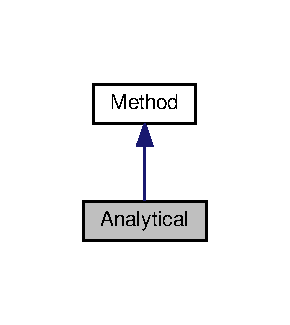
\includegraphics[width=215pt]{classAnalytical__inherit__graph}
\end{center}
\end{figure}


Collaboration diagram for Analytical\+:
\nopagebreak
\begin{figure}[H]
\begin{center}
\leavevmode
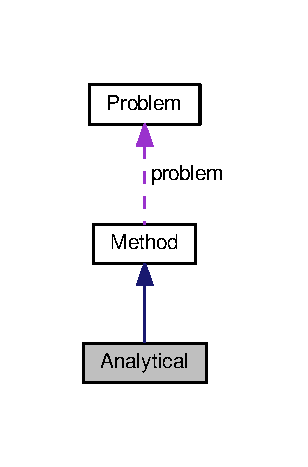
\includegraphics[height=550pt]{classAnalytical__coll__graph}
\end{center}
\end{figure}
\subsection*{Public Member Functions}
\begin{DoxyCompactItemize}
\item 
\hyperlink{classAnalytical_a04b2afb565db2e19293799c169e42adb}{Analytical} (\hyperlink{classProblem}{Problem} \hyperlink{classMethod_a29a08a679b5d30a8c813766308205041}{problem})
\begin{DoxyCompactList}\small\item\em Default constructor. \end{DoxyCompactList}\item 
void \hyperlink{classAnalytical_a48b4e86fd33f1dfd9f59b470cc1272a6}{compute\+\_\+solution} ()
\begin{DoxyCompactList}\small\item\em Normal public method. \end{DoxyCompactList}\end{DoxyCompactItemize}
\subsection*{Private Attributes}
\begin{DoxyCompactItemize}
\item 
unsigned int \hyperlink{classAnalytical_a853d708e2c746c3b81df14770594b76a}{nr\+\_\+of\+\_\+expansions}
\begin{DoxyCompactList}\small\item\em Private unsigned int nr\+\_\+of\+\_\+expansions. \end{DoxyCompactList}\end{DoxyCompactItemize}
\subsection*{Additional Inherited Members}


\subsection{Detailed Description}
An \hyperlink{classAnalytical}{Analytical} class to compute the solution with standard procedures ~\newline
 The implementation is derived from the \hyperlink{classMethod}{Method} Object. 

The \hyperlink{classAnalytical}{Analytical} class provides\+: ~\newline
-\/a basic constructor for an object, ~\newline
-\/a method to compute a solution with the correct procedures 

\subsection{Constructor \& Destructor Documentation}
\index{Analytical@{Analytical}!Analytical@{Analytical}}
\index{Analytical@{Analytical}!Analytical@{Analytical}}
\subsubsection[{\texorpdfstring{Analytical(\+Problem problem)}{Analytical(Problem problem)}}]{\setlength{\rightskip}{0pt plus 5cm}Analytical\+::\+Analytical (
\begin{DoxyParamCaption}
\item[{{\bf Problem}}]{problem}
\end{DoxyParamCaption}
)}\hypertarget{classAnalytical_a04b2afb565db2e19293799c169e42adb}{}\label{classAnalytical_a04b2afb565db2e19293799c169e42adb}


Default constructor. 

Intialize a \hyperlink{classAnalytical}{Analytical} object 

\subsection{Member Function Documentation}
\index{Analytical@{Analytical}!compute\+\_\+solution@{compute\+\_\+solution}}
\index{compute\+\_\+solution@{compute\+\_\+solution}!Analytical@{Analytical}}
\subsubsection[{\texorpdfstring{compute\+\_\+solution()}{compute_solution()}}]{\setlength{\rightskip}{0pt plus 5cm}void Analytical\+::compute\+\_\+solution (
\begin{DoxyParamCaption}
{}
\end{DoxyParamCaption}
)\hspace{0.3cm}{\ttfamily [virtual]}}\hypertarget{classAnalytical_a48b4e86fd33f1dfd9f59b470cc1272a6}{}\label{classAnalytical_a48b4e86fd33f1dfd9f59b470cc1272a6}


Normal public method. 

compute the solution with specific given rules 

Implements \hyperlink{classMethod_af3dcec8e066214e82d8b4578a4a55076}{Method}.



Here is the call graph for this function\+:
\nopagebreak
\begin{figure}[H]
\begin{center}
\leavevmode
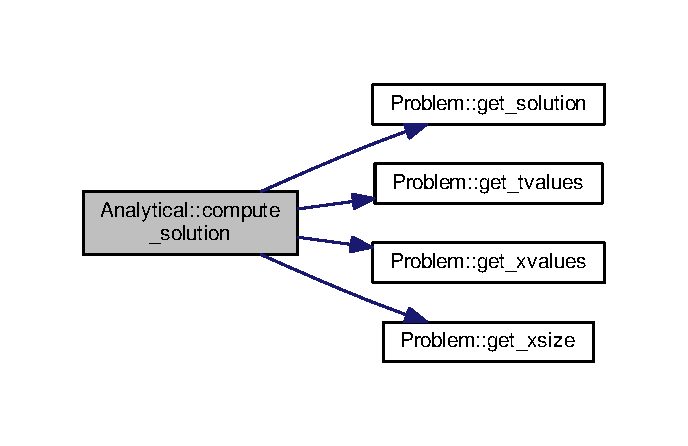
\includegraphics[width=330pt]{classAnalytical_a48b4e86fd33f1dfd9f59b470cc1272a6_cgraph}
\end{center}
\end{figure}




\subsection{Member Data Documentation}
\index{Analytical@{Analytical}!nr\+\_\+of\+\_\+expansions@{nr\+\_\+of\+\_\+expansions}}
\index{nr\+\_\+of\+\_\+expansions@{nr\+\_\+of\+\_\+expansions}!Analytical@{Analytical}}
\subsubsection[{\texorpdfstring{nr\+\_\+of\+\_\+expansions}{nr_of_expansions}}]{\setlength{\rightskip}{0pt plus 5cm}unsigned int Analytical\+::nr\+\_\+of\+\_\+expansions\hspace{0.3cm}{\ttfamily [private]}}\hypertarget{classAnalytical_a853d708e2c746c3b81df14770594b76a}{}\label{classAnalytical_a853d708e2c746c3b81df14770594b76a}


Private unsigned int nr\+\_\+of\+\_\+expansions. 

Limit of expansions to do in the sum used to compute the solution. 

The documentation for this class was generated from the following files\+:\begin{DoxyCompactItemize}
\item 
methods/\hyperlink{analytical_8h}{analytical.\+h}\item 
methods/\hyperlink{analytical_8cpp}{analytical.\+cpp}\end{DoxyCompactItemize}

\hypertarget{classCrankNicolson}{}\section{Crank\+Nicolson Class Reference}
\label{classCrankNicolson}\index{Crank\+Nicolson@{Crank\+Nicolson}}


A \hyperlink{classCrankNicolson}{Crank\+Nicolson} method class that contains a r vector builder.  




{\ttfamily \#include $<$crank\+\_\+nicolson.\+h$>$}



Inheritance diagram for Crank\+Nicolson\+:
\nopagebreak
\begin{figure}[H]
\begin{center}
\leavevmode
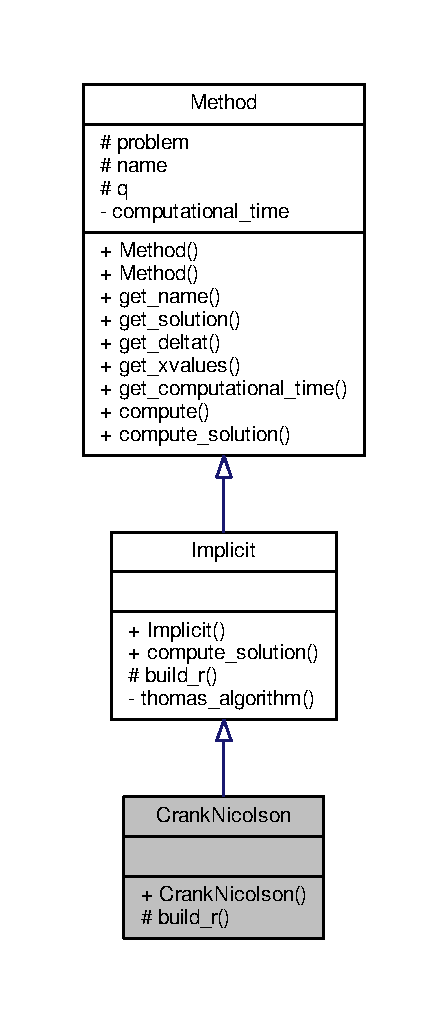
\includegraphics[width=215pt]{classCrankNicolson__inherit__graph}
\end{center}
\end{figure}


Collaboration diagram for Crank\+Nicolson\+:
\nopagebreak
\begin{figure}[H]
\begin{center}
\leavevmode
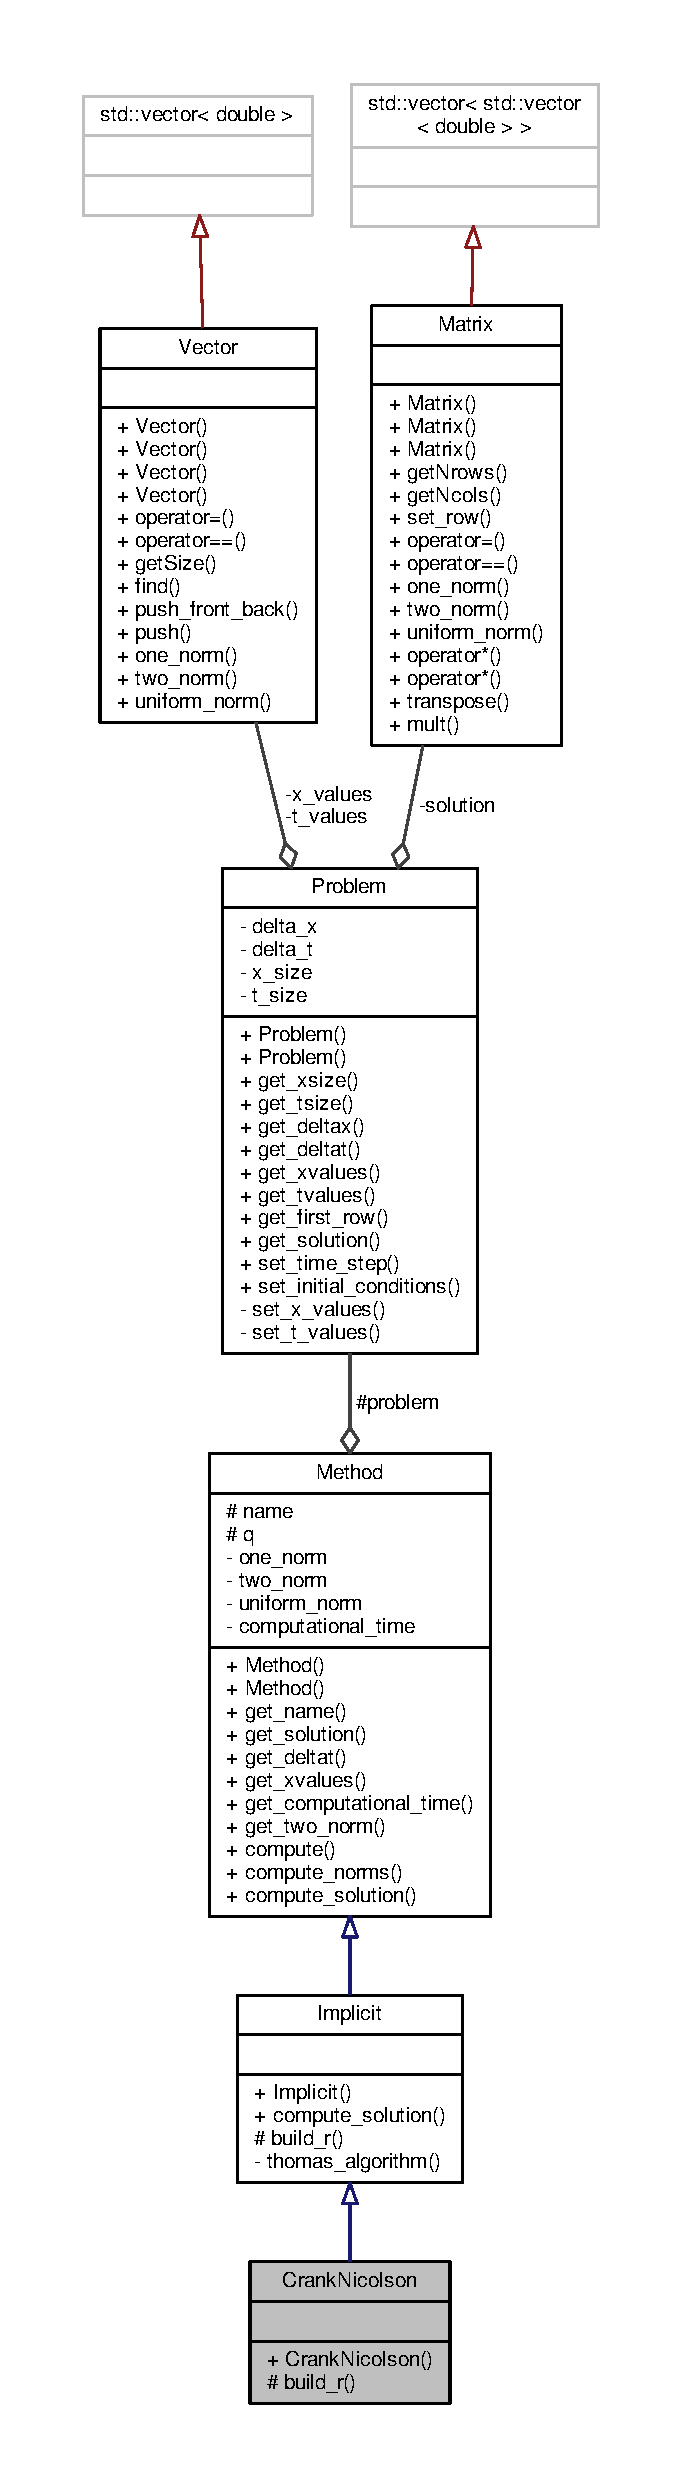
\includegraphics[height=550pt]{classCrankNicolson__coll__graph}
\end{center}
\end{figure}
\subsection*{Public Member Functions}
\begin{DoxyCompactItemize}
\item 
\hyperlink{classCrankNicolson_a57f6bedf8527a32e39a2384ef448e417}{Crank\+Nicolson} (\hyperlink{classProblem}{Problem} \hyperlink{classMethod_a29a08a679b5d30a8c813766308205041}{problem})
\begin{DoxyCompactList}\small\item\em Default constructor. \end{DoxyCompactList}\end{DoxyCompactItemize}
\subsection*{Protected Member Functions}
\begin{DoxyCompactItemize}
\item 
\hyperlink{classVector}{Vector} \hyperlink{classCrankNicolson_a9b67095f05b0ee96701d6cd38099f6c4}{build\+\_\+r} (\hyperlink{classVector}{Vector} previous\+\_\+step)
\begin{DoxyCompactList}\small\item\em Normal protected method. \end{DoxyCompactList}\end{DoxyCompactItemize}
\subsection*{Additional Inherited Members}


\subsection{Detailed Description}
A \hyperlink{classCrankNicolson}{Crank\+Nicolson} method class that contains a r vector builder. 

~\newline
 This builder is used to calculate the r vector in A.\+x = r linear equation system.

The \hyperlink{classCrankNicolson}{Crank\+Nicolson} class provides\+: ~\newline
-\/a basic constructor for creating a \hyperlink{classCrankNicolson}{Crank\+Nicolson} method object. ~\newline
-\/a method to compute the r vector. 

\subsection{Constructor \& Destructor Documentation}
\index{Crank\+Nicolson@{Crank\+Nicolson}!Crank\+Nicolson@{Crank\+Nicolson}}
\index{Crank\+Nicolson@{Crank\+Nicolson}!Crank\+Nicolson@{Crank\+Nicolson}}
\subsubsection[{\texorpdfstring{Crank\+Nicolson(\+Problem problem)}{CrankNicolson(Problem problem)}}]{\setlength{\rightskip}{0pt plus 5cm}Crank\+Nicolson\+::\+Crank\+Nicolson (
\begin{DoxyParamCaption}
\item[{{\bf Problem}}]{problem}
\end{DoxyParamCaption}
)}\hypertarget{classCrankNicolson_a57f6bedf8527a32e39a2384ef448e417}{}\label{classCrankNicolson_a57f6bedf8527a32e39a2384ef448e417}


Default constructor. 



\subsection{Member Function Documentation}
\index{Crank\+Nicolson@{Crank\+Nicolson}!build\+\_\+r@{build\+\_\+r}}
\index{build\+\_\+r@{build\+\_\+r}!Crank\+Nicolson@{Crank\+Nicolson}}
\subsubsection[{\texorpdfstring{build\+\_\+r(\+Vector previous\+\_\+step)}{build_r(Vector previous_step)}}]{\setlength{\rightskip}{0pt plus 5cm}{\bf Vector} Crank\+Nicolson\+::build\+\_\+r (
\begin{DoxyParamCaption}
\item[{{\bf Vector}}]{previous\+\_\+step}
\end{DoxyParamCaption}
)\hspace{0.3cm}{\ttfamily [protected]}, {\ttfamily [virtual]}}\hypertarget{classCrankNicolson_a9b67095f05b0ee96701d6cd38099f6c4}{}\label{classCrankNicolson_a9b67095f05b0ee96701d6cd38099f6c4}


Normal protected method. 

get the number of rows 
\begin{DoxyParams}{Parameters}
{\em previous\+\_\+step} & \hyperlink{classVector}{Vector} representing the solution of the previous time step. \\
\hline
\end{DoxyParams}
\begin{DoxyReturn}{Returns}
\hyperlink{classVector}{Vector}. r vector to be used in A.\+x = r 
\end{DoxyReturn}


Implements \hyperlink{classImplicit_ab2d07b5185008b2c845a31a03350d98d}{Implicit}.



Here is the call graph for this function\+:
\nopagebreak
\begin{figure}[H]
\begin{center}
\leavevmode
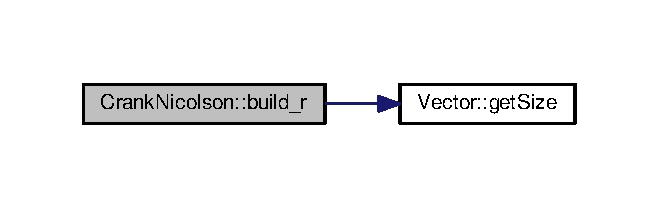
\includegraphics[width=316pt]{classCrankNicolson_a9b67095f05b0ee96701d6cd38099f6c4_cgraph}
\end{center}
\end{figure}




The documentation for this class was generated from the following files\+:\begin{DoxyCompactItemize}
\item 
methods/implicit/\hyperlink{crank__nicolson_8h}{crank\+\_\+nicolson.\+h}\item 
methods/implicit/\hyperlink{crank__nicolson_8cpp}{crank\+\_\+nicolson.\+cpp}\end{DoxyCompactItemize}

\hypertarget{classDufortFrankel}{}\section{Dufort\+Frankel Class Reference}
\label{classDufortFrankel}\index{Dufort\+Frankel@{Dufort\+Frankel}}


{\ttfamily \#include $<$dufort\+\_\+frankel.\+h$>$}



Inheritance diagram for Dufort\+Frankel\+:
\nopagebreak
\begin{figure}[H]
\begin{center}
\leavevmode
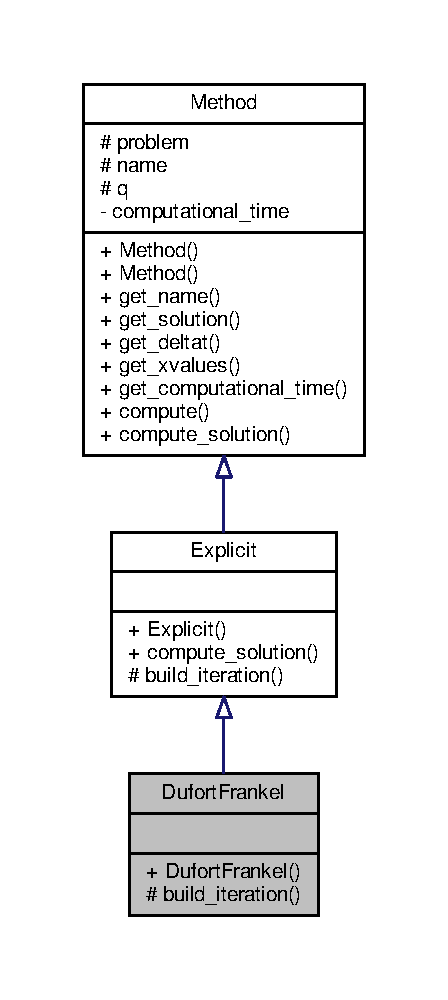
\includegraphics[width=156pt]{classDufortFrankel__inherit__graph}
\end{center}
\end{figure}


Collaboration diagram for Dufort\+Frankel\+:
\nopagebreak
\begin{figure}[H]
\begin{center}
\leavevmode
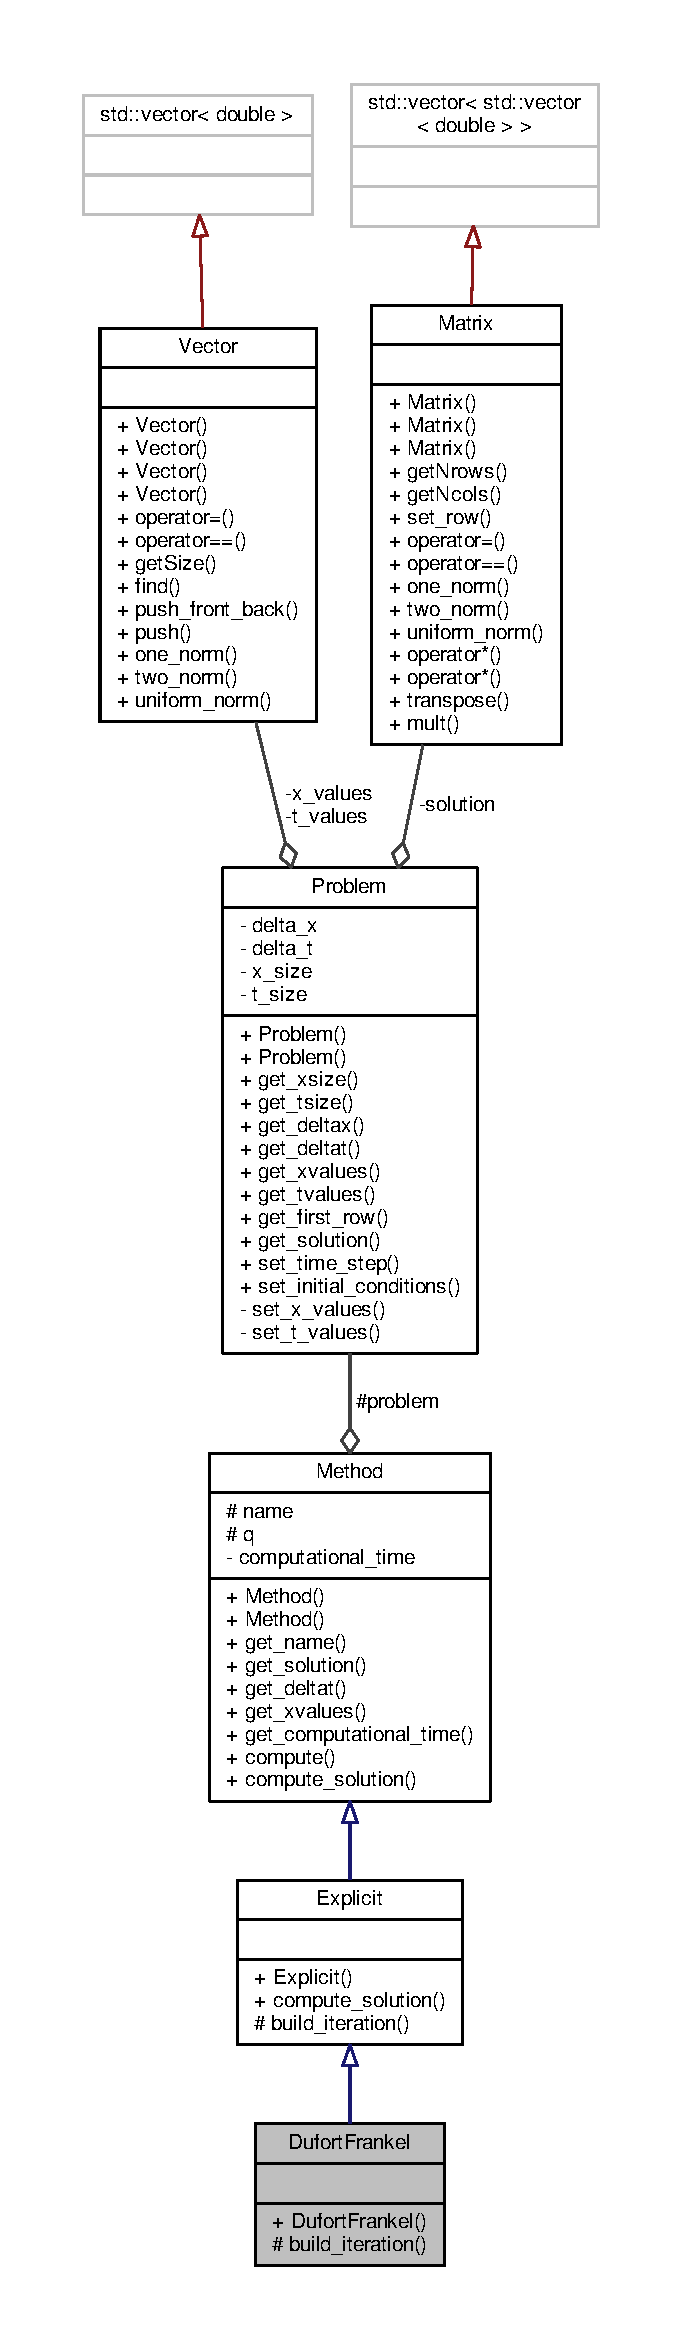
\includegraphics[width=156pt]{classDufortFrankel__coll__graph}
\end{center}
\end{figure}
\subsection*{Public Member Functions}
\begin{DoxyCompactItemize}
\item 
\hyperlink{classDufortFrankel_a3da0cebb23f1c23c8656b5d39824b22b}{Dufort\+Frankel} (\hyperlink{classProblem}{Problem} \hyperlink{classMethod_a29a08a679b5d30a8c813766308205041}{problem})
\end{DoxyCompactItemize}
\subsection*{Protected Member Functions}
\begin{DoxyCompactItemize}
\item 
\hyperlink{classVector}{Vector} \hyperlink{classDufortFrankel_ae140760ed55ca045a2136e6e882cecd4}{build\+\_\+iteration} (\hyperlink{classVector}{Vector} current\+\_\+step, \hyperlink{classVector}{Vector} previous\+\_\+step)
\end{DoxyCompactItemize}
\subsection*{Additional Inherited Members}


\subsection{Detailed Description}
A \hyperlink{classDufortFrankel}{Dufort\+Frankel} method class that contains an iteration builder. ~\newline
 This builder is used to calculate a solution using the Dufort-\/\+Frankel mathod.

The \hyperlink{classDufortFrankel}{Dufort\+Frankel} class provides\+: ~\newline
-\/a basic constructor for creating a \hyperlink{classDufortFrankel}{Dufort\+Frankel} method object. ~\newline
-\/a method to compute a solution of the current iteration 

\subsection{Constructor \& Destructor Documentation}
\index{Dufort\+Frankel@{Dufort\+Frankel}!Dufort\+Frankel@{Dufort\+Frankel}}
\index{Dufort\+Frankel@{Dufort\+Frankel}!Dufort\+Frankel@{Dufort\+Frankel}}
\subsubsection[{\texorpdfstring{Dufort\+Frankel(\+Problem problem)}{DufortFrankel(Problem problem)}}]{\setlength{\rightskip}{0pt plus 5cm}Dufort\+Frankel\+::\+Dufort\+Frankel (
\begin{DoxyParamCaption}
\item[{{\bf Problem}}]{problem}
\end{DoxyParamCaption}
)}\hypertarget{classDufortFrankel_a3da0cebb23f1c23c8656b5d39824b22b}{}\label{classDufortFrankel_a3da0cebb23f1c23c8656b5d39824b22b}
Default constructor. 

\subsection{Member Function Documentation}
\index{Dufort\+Frankel@{Dufort\+Frankel}!build\+\_\+iteration@{build\+\_\+iteration}}
\index{build\+\_\+iteration@{build\+\_\+iteration}!Dufort\+Frankel@{Dufort\+Frankel}}
\subsubsection[{\texorpdfstring{build\+\_\+iteration(\+Vector current\+\_\+step, Vector previous\+\_\+step)}{build_iteration(Vector current_step, Vector previous_step)}}]{\setlength{\rightskip}{0pt plus 5cm}{\bf Vector} Dufort\+Frankel\+::build\+\_\+iteration (
\begin{DoxyParamCaption}
\item[{{\bf Vector}}]{current\+\_\+step, }
\item[{{\bf Vector}}]{previous\+\_\+step}
\end{DoxyParamCaption}
)\hspace{0.3cm}{\ttfamily [protected]}, {\ttfamily [virtual]}}\hypertarget{classDufortFrankel_ae140760ed55ca045a2136e6e882cecd4}{}\label{classDufortFrankel_ae140760ed55ca045a2136e6e882cecd4}
Normal protected method. Calculate a next time step solution requiring a previous time step and a current time step solution. 
\begin{DoxyParams}{Parameters}
{\em current\+\_\+step} & A vector representing the current time step solution. \\
\hline
{\em previous\+\_\+step} & A vector representing the previous time step solution. \\
\hline
\end{DoxyParams}
\begin{DoxyReturn}{Returns}
\hyperlink{classVector}{Vector}. The computed solution. 
\end{DoxyReturn}


Implements \hyperlink{classExplicit_a2b9b097253488f4ce07a8ef0580a5d22}{Explicit}.



The documentation for this class was generated from the following files\+:\begin{DoxyCompactItemize}
\item 
methods/explicit/dufort\+\_\+frankel.\+h\item 
methods/explicit/dufort\+\_\+frankel.\+cpp\end{DoxyCompactItemize}

\hypertarget{classExplicit}{}\section{Explicit Class Reference}
\label{classExplicit}\index{Explicit@{Explicit}}


An explicit method class that contains default methods that only explicit methods use ~\newline
 The implementation is derived from the \hyperlink{classMethod}{Method} class.  




{\ttfamily \#include $<$explicit.\+h$>$}



Inheritance diagram for Explicit\+:
\nopagebreak
\begin{figure}[H]
\begin{center}
\leavevmode
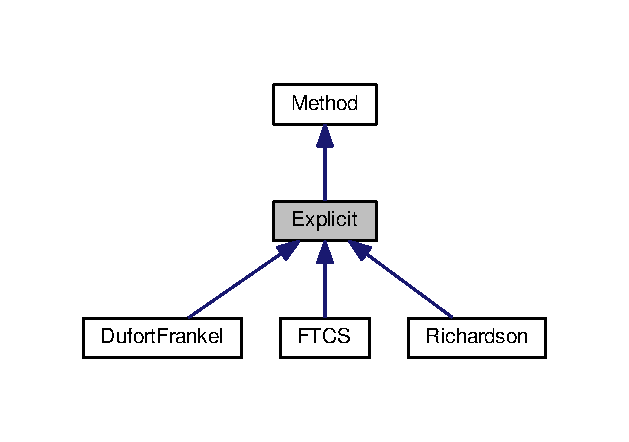
\includegraphics[width=350pt]{classExplicit__inherit__graph}
\end{center}
\end{figure}


Collaboration diagram for Explicit\+:
\nopagebreak
\begin{figure}[H]
\begin{center}
\leavevmode
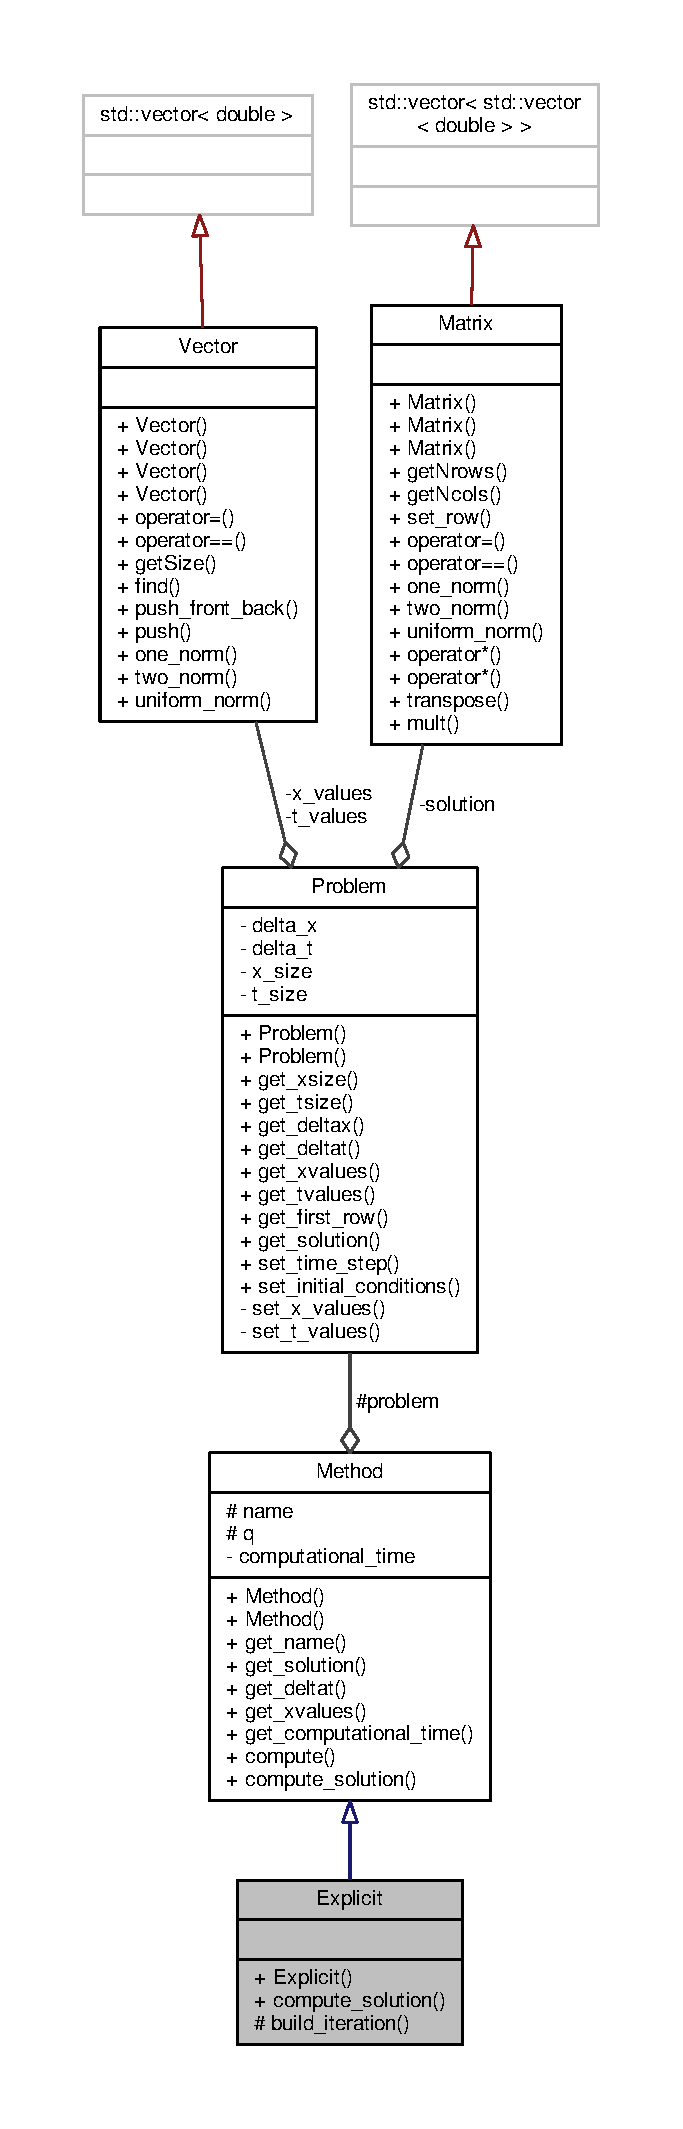
\includegraphics[height=550pt]{classExplicit__coll__graph}
\end{center}
\end{figure}
\subsection*{Public Member Functions}
\begin{DoxyCompactItemize}
\item 
\hyperlink{classExplicit_a87a81a730d68689268204ae8b296075d}{Explicit} (\hyperlink{classProblem}{Problem} \hyperlink{classMethod_a29a08a679b5d30a8c813766308205041}{problem})
\begin{DoxyCompactList}\small\item\em Default constructor. \end{DoxyCompactList}\item 
void \hyperlink{classExplicit_a09fa3df66e16200fefaabc908e6efafd}{compute\+\_\+solution} ()
\begin{DoxyCompactList}\small\item\em Normal public method. \end{DoxyCompactList}\end{DoxyCompactItemize}
\subsection*{Protected Member Functions}
\begin{DoxyCompactItemize}
\item 
virtual \hyperlink{classVector}{Vector} \hyperlink{classExplicit_a2b9b097253488f4ce07a8ef0580a5d22}{build\+\_\+iteration} (\hyperlink{classVector}{Vector} current\+\_\+step, \hyperlink{classVector}{Vector} previous\+\_\+step)=0
\begin{DoxyCompactList}\small\item\em A pure virtual member. \end{DoxyCompactList}\end{DoxyCompactItemize}
\subsection*{Additional Inherited Members}


\subsection{Detailed Description}
An explicit method class that contains default methods that only explicit methods use ~\newline
 The implementation is derived from the \hyperlink{classMethod}{Method} class. 

The \hyperlink{classExplicit}{Explicit} class provides\+: ~\newline
-\/a basic constructor for creating an explicit method object. ~\newline
-\/a method to compute a solution following explicit methods rules 

\subsection{Constructor \& Destructor Documentation}
\index{Explicit@{Explicit}!Explicit@{Explicit}}
\index{Explicit@{Explicit}!Explicit@{Explicit}}
\subsubsection[{\texorpdfstring{Explicit(\+Problem problem)}{Explicit(Problem problem)}}]{\setlength{\rightskip}{0pt plus 5cm}Explicit\+::\+Explicit (
\begin{DoxyParamCaption}
\item[{{\bf Problem}}]{problem}
\end{DoxyParamCaption}
)}\hypertarget{classExplicit_a87a81a730d68689268204ae8b296075d}{}\label{classExplicit_a87a81a730d68689268204ae8b296075d}


Default constructor. 



Here is the call graph for this function\+:
\nopagebreak
\begin{figure}[H]
\begin{center}
\leavevmode
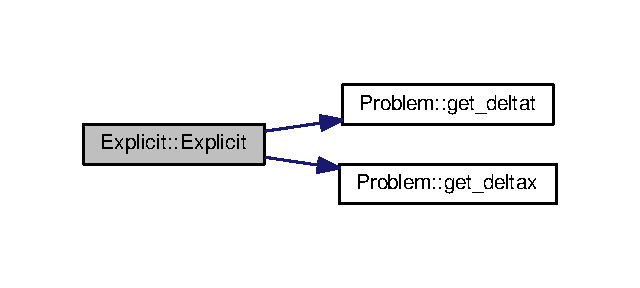
\includegraphics[width=307pt]{classExplicit_a87a81a730d68689268204ae8b296075d_cgraph}
\end{center}
\end{figure}




\subsection{Member Function Documentation}
\index{Explicit@{Explicit}!build\+\_\+iteration@{build\+\_\+iteration}}
\index{build\+\_\+iteration@{build\+\_\+iteration}!Explicit@{Explicit}}
\subsubsection[{\texorpdfstring{build\+\_\+iteration(\+Vector current\+\_\+step, Vector previous\+\_\+step)=0}{build_iteration(Vector current_step, Vector previous_step)=0}}]{\setlength{\rightskip}{0pt plus 5cm}virtual {\bf Vector} Explicit\+::build\+\_\+iteration (
\begin{DoxyParamCaption}
\item[{{\bf Vector}}]{current\+\_\+step, }
\item[{{\bf Vector}}]{previous\+\_\+step}
\end{DoxyParamCaption}
)\hspace{0.3cm}{\ttfamily [protected]}, {\ttfamily [pure virtual]}}\hypertarget{classExplicit_a2b9b097253488f4ce07a8ef0580a5d22}{}\label{classExplicit_a2b9b097253488f4ce07a8ef0580a5d22}


A pure virtual member. 

Build the solution of the next time step, using the previous time step and the next time step solutions 
\begin{DoxyParams}{Parameters}
{\em previous\+\_\+step} & A vector containing the previous time step solution. \\
\hline
{\em current\+\_\+step} & A vector containing the current time step solution. \\
\hline
\end{DoxyParams}
\begin{DoxyReturn}{Returns}
\hyperlink{classVector}{Vector}. A vector representing the next time step solution. 
\end{DoxyReturn}


Implemented in \hyperlink{classFTCS_abc8074dbb5a5facaf0380aa867998556}{F\+T\+CS}, \hyperlink{classDufortFrankel_ae140760ed55ca045a2136e6e882cecd4}{Dufort\+Frankel}, and \hyperlink{classRichardson_a310f998254af88c3ad7532411b11a5fb}{Richardson}.



Here is the caller graph for this function\+:
\nopagebreak
\begin{figure}[H]
\begin{center}
\leavevmode
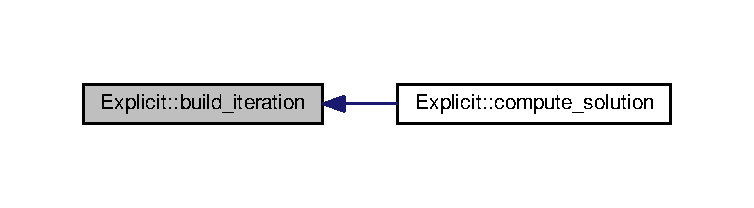
\includegraphics[width=350pt]{classExplicit_a2b9b097253488f4ce07a8ef0580a5d22_icgraph}
\end{center}
\end{figure}


\index{Explicit@{Explicit}!compute\+\_\+solution@{compute\+\_\+solution}}
\index{compute\+\_\+solution@{compute\+\_\+solution}!Explicit@{Explicit}}
\subsubsection[{\texorpdfstring{compute\+\_\+solution()}{compute_solution()}}]{\setlength{\rightskip}{0pt plus 5cm}void Explicit\+::compute\+\_\+solution (
\begin{DoxyParamCaption}
{}
\end{DoxyParamCaption}
)\hspace{0.3cm}{\ttfamily [virtual]}}\hypertarget{classExplicit_a09fa3df66e16200fefaabc908e6efafd}{}\label{classExplicit_a09fa3df66e16200fefaabc908e6efafd}


Normal public method. 

Calculates a solution for the given problem by populating the solution grid with the correct values. 

Implements \hyperlink{classMethod_af3dcec8e066214e82d8b4578a4a55076}{Method}.



Here is the call graph for this function\+:
\nopagebreak
\begin{figure}[H]
\begin{center}
\leavevmode
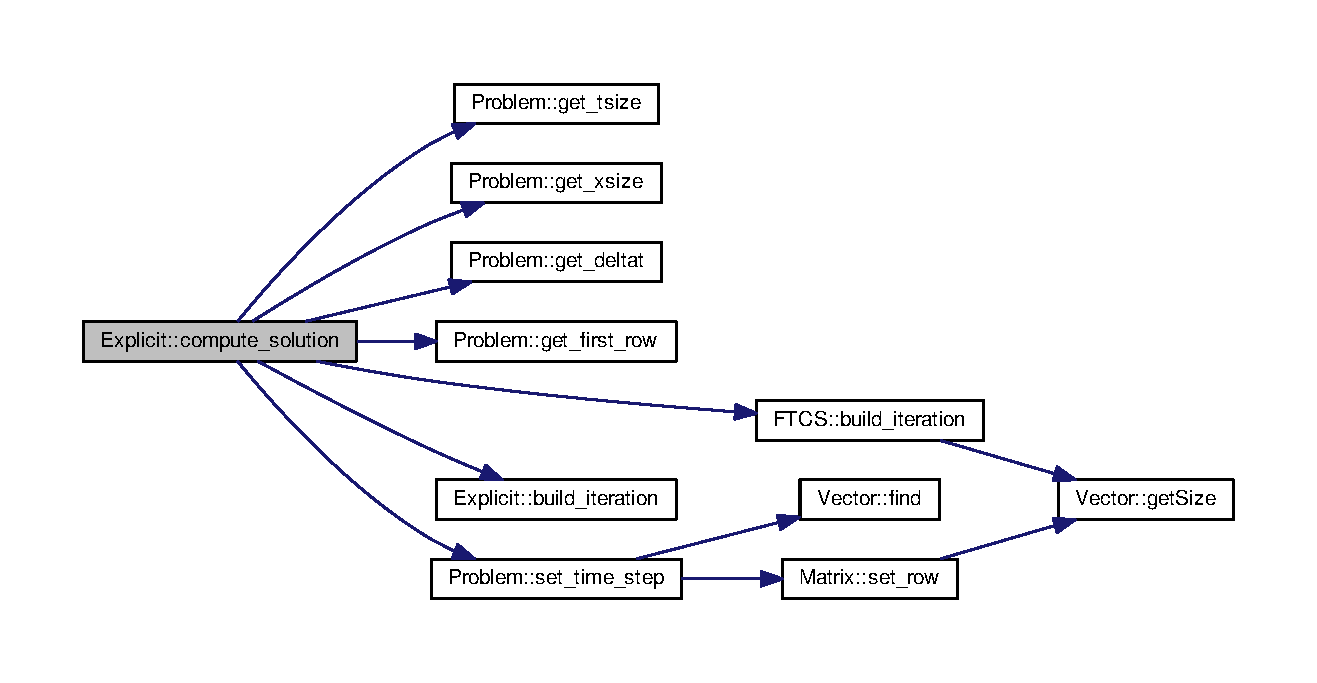
\includegraphics[width=350pt]{classExplicit_a09fa3df66e16200fefaabc908e6efafd_cgraph}
\end{center}
\end{figure}




The documentation for this class was generated from the following files\+:\begin{DoxyCompactItemize}
\item 
methods/explicit/\hyperlink{explicit_8h}{explicit.\+h}\item 
methods/explicit/\hyperlink{explicit_8cpp}{explicit.\+cpp}\end{DoxyCompactItemize}

\hypertarget{classFTCS}{}\section{F\+T\+CS Class Reference}
\label{classFTCS}\index{F\+T\+CS@{F\+T\+CS}}


A \hyperlink{classFTCS}{F\+T\+CS} method class that contains an iteration builder.  




{\ttfamily \#include $<$forward\+\_\+t\+\_\+central\+\_\+s.\+h$>$}



Inheritance diagram for F\+T\+CS\+:
\nopagebreak
\begin{figure}[H]
\begin{center}
\leavevmode
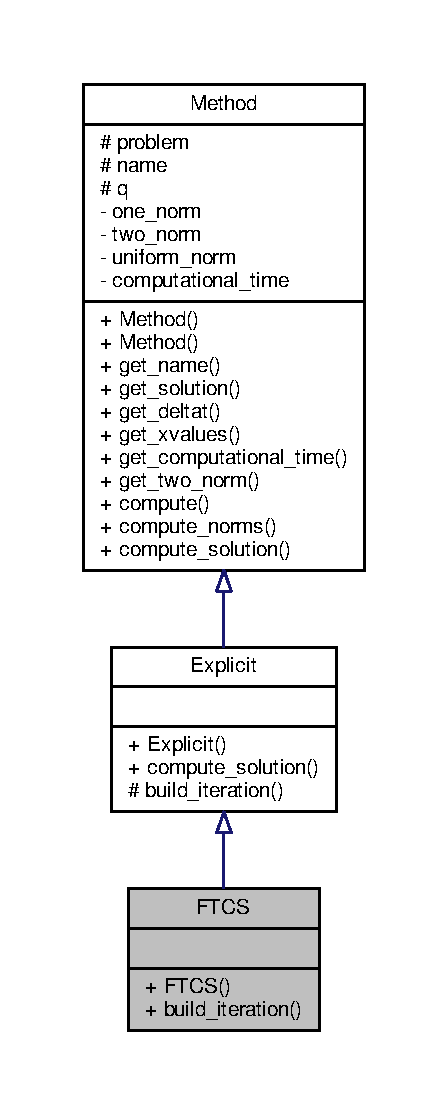
\includegraphics[width=215pt]{classFTCS__inherit__graph}
\end{center}
\end{figure}


Collaboration diagram for F\+T\+CS\+:
\nopagebreak
\begin{figure}[H]
\begin{center}
\leavevmode
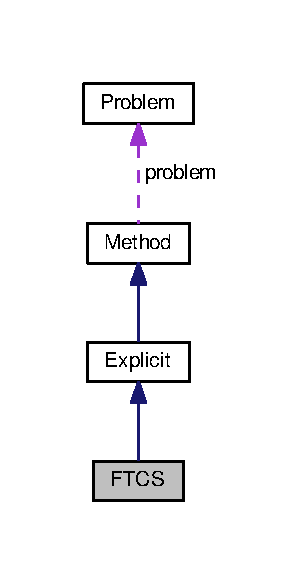
\includegraphics[height=550pt]{classFTCS__coll__graph}
\end{center}
\end{figure}
\subsection*{Public Member Functions}
\begin{DoxyCompactItemize}
\item 
\hyperlink{classFTCS_a7a41ea5217c29d68cebf1a5e20effa8b}{F\+T\+CS} (\hyperlink{classProblem}{Problem} \hyperlink{classMethod_a29a08a679b5d30a8c813766308205041}{problem})
\begin{DoxyCompactList}\small\item\em Default constructor. \end{DoxyCompactList}\item 
\hyperlink{classVector}{Vector} \hyperlink{classFTCS_abc8074dbb5a5facaf0380aa867998556}{build\+\_\+iteration} (\hyperlink{classVector}{Vector} current\+\_\+step, \hyperlink{classVector}{Vector} previous\+\_\+step)
\begin{DoxyCompactList}\small\item\em Normal public method. \end{DoxyCompactList}\end{DoxyCompactItemize}
\subsection*{Additional Inherited Members}


\subsection{Detailed Description}
A \hyperlink{classFTCS}{F\+T\+CS} method class that contains an iteration builder. 

~\newline
 This builder is used to calculate the first iteration of explicit methods, since it only requires the previous step solution to do it.

The \hyperlink{classFTCS}{F\+T\+CS} class provides\+: ~\newline
-\/a basic constructor for creating a \hyperlink{classFTCS}{F\+T\+CS} method object. ~\newline
-\/a method to compute the current iteration 

\subsection{Constructor \& Destructor Documentation}
\index{F\+T\+CS@{F\+T\+CS}!F\+T\+CS@{F\+T\+CS}}
\index{F\+T\+CS@{F\+T\+CS}!F\+T\+CS@{F\+T\+CS}}
\subsubsection[{\texorpdfstring{F\+T\+C\+S(\+Problem problem)}{FTCS(Problem problem)}}]{\setlength{\rightskip}{0pt plus 5cm}F\+T\+C\+S\+::\+F\+T\+CS (
\begin{DoxyParamCaption}
\item[{{\bf Problem}}]{problem}
\end{DoxyParamCaption}
)}\hypertarget{classFTCS_a7a41ea5217c29d68cebf1a5e20effa8b}{}\label{classFTCS_a7a41ea5217c29d68cebf1a5e20effa8b}


Default constructor. 



\subsection{Member Function Documentation}
\index{F\+T\+CS@{F\+T\+CS}!build\+\_\+iteration@{build\+\_\+iteration}}
\index{build\+\_\+iteration@{build\+\_\+iteration}!F\+T\+CS@{F\+T\+CS}}
\subsubsection[{\texorpdfstring{build\+\_\+iteration(\+Vector current\+\_\+step, Vector previous\+\_\+step)}{build_iteration(Vector current_step, Vector previous_step)}}]{\setlength{\rightskip}{0pt plus 5cm}{\bf Vector} F\+T\+C\+S\+::build\+\_\+iteration (
\begin{DoxyParamCaption}
\item[{{\bf Vector}}]{current\+\_\+step, }
\item[{{\bf Vector}}]{previous\+\_\+step}
\end{DoxyParamCaption}
)\hspace{0.3cm}{\ttfamily [virtual]}}\hypertarget{classFTCS_abc8074dbb5a5facaf0380aa867998556}{}\label{classFTCS_abc8074dbb5a5facaf0380aa867998556}


Normal public method. 

Calculate a solution requiring only the previous time step solution. 
\begin{DoxyParams}{Parameters}
{\em current\+\_\+step} & A vector with size 0, it\textquotesingle{}s not required in this method. \\
\hline
{\em previous\+\_\+step} & A vector representing the previous time step solution \\
\hline
\end{DoxyParams}
\begin{DoxyReturn}{Returns}
\hyperlink{classVector}{Vector}. The computed solution. 
\end{DoxyReturn}


Implements \hyperlink{classExplicit_a2b9b097253488f4ce07a8ef0580a5d22}{Explicit}.



Here is the call graph for this function\+:
\nopagebreak
\begin{figure}[H]
\begin{center}
\leavevmode
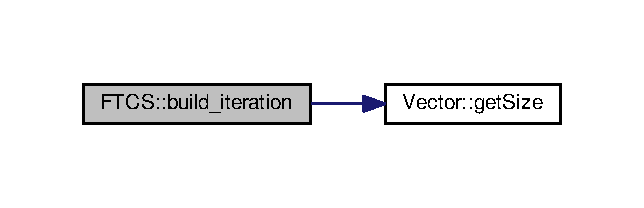
\includegraphics[width=309pt]{classFTCS_abc8074dbb5a5facaf0380aa867998556_cgraph}
\end{center}
\end{figure}




Here is the caller graph for this function\+:
\nopagebreak
\begin{figure}[H]
\begin{center}
\leavevmode
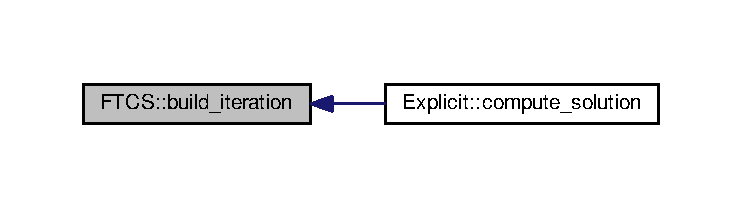
\includegraphics[width=350pt]{classFTCS_abc8074dbb5a5facaf0380aa867998556_icgraph}
\end{center}
\end{figure}




The documentation for this class was generated from the following files\+:\begin{DoxyCompactItemize}
\item 
methods/explicit/\hyperlink{forward__t__central__s_8h}{forward\+\_\+t\+\_\+central\+\_\+s.\+h}\item 
methods/explicit/\hyperlink{forward__t__central__s_8cpp}{forward\+\_\+t\+\_\+central\+\_\+s.\+cpp}\end{DoxyCompactItemize}

\hypertarget{classImplicit}{}\section{Implicit Class Reference}
\label{classImplicit}\index{Implicit@{Implicit}}


An implicit method class that contains default methods that only implicit methods use ~\newline
 The implementation is derived from the \hyperlink{classMethod}{Method} class.  




{\ttfamily \#include $<$implicit.\+h$>$}



Inheritance diagram for Implicit\+:
\nopagebreak
\begin{figure}[H]
\begin{center}
\leavevmode
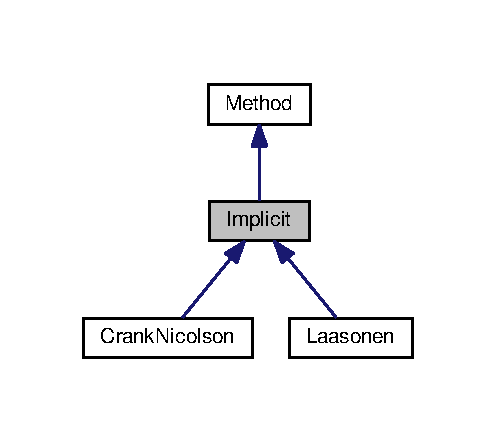
\includegraphics[width=268pt]{classImplicit__inherit__graph}
\end{center}
\end{figure}


Collaboration diagram for Implicit\+:
\nopagebreak
\begin{figure}[H]
\begin{center}
\leavevmode
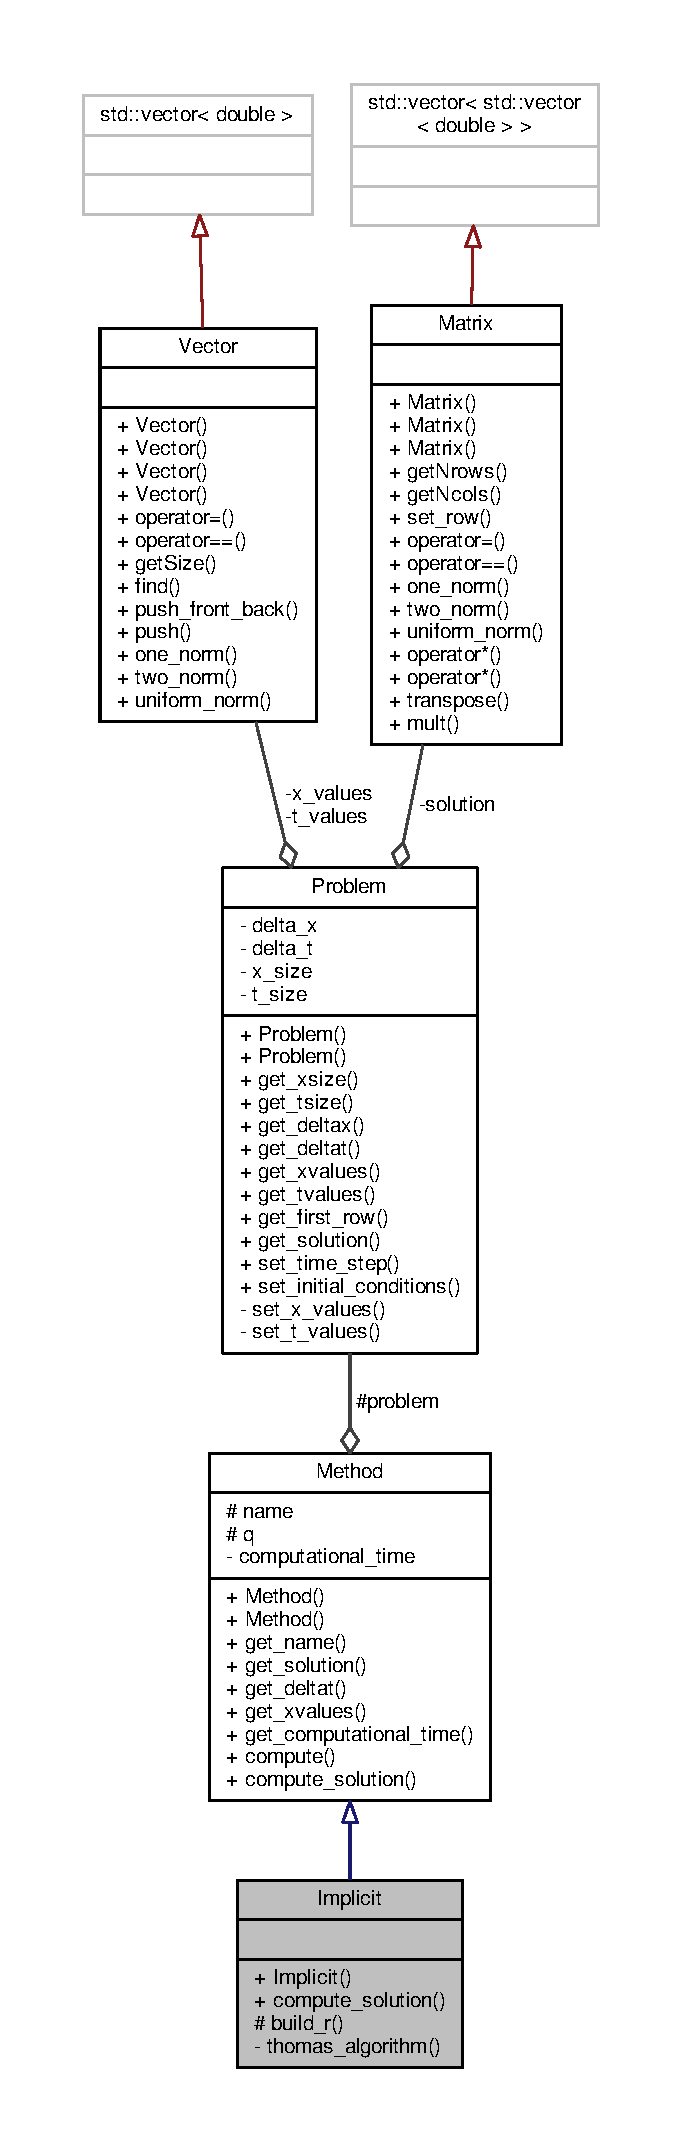
\includegraphics[height=550pt]{classImplicit__coll__graph}
\end{center}
\end{figure}
\subsection*{Public Member Functions}
\begin{DoxyCompactItemize}
\item 
\hyperlink{classImplicit_a5bc81959cd5329526f1c2b7e6e050050}{Implicit} (\hyperlink{classProblem}{Problem} \hyperlink{classMethod_a29a08a679b5d30a8c813766308205041}{problem})
\begin{DoxyCompactList}\small\item\em Default constructor. \end{DoxyCompactList}\item 
void \hyperlink{classImplicit_a1d6b7250da6d3a417baefe7328635d45}{compute\+\_\+solution} ()
\begin{DoxyCompactList}\small\item\em Normal public method. \end{DoxyCompactList}\end{DoxyCompactItemize}
\subsection*{Protected Member Functions}
\begin{DoxyCompactItemize}
\item 
virtual \hyperlink{classVector}{Vector} \hyperlink{classImplicit_ab2d07b5185008b2c845a31a03350d98d}{build\+\_\+r} (\hyperlink{classVector}{Vector} previous\+\_\+step)=0
\begin{DoxyCompactList}\small\item\em A pure virtual member. \end{DoxyCompactList}\end{DoxyCompactItemize}
\subsection*{Private Member Functions}
\begin{DoxyCompactItemize}
\item 
\hyperlink{classVector}{Vector} \hyperlink{classImplicit_a095e8555a718b53ff94770a0a220dfba}{thomas\+\_\+algorithm} (\hyperlink{classVector}{Vector} r, double a, double b, double c)
\begin{DoxyCompactList}\small\item\em Normal private method. \end{DoxyCompactList}\end{DoxyCompactItemize}
\subsection*{Additional Inherited Members}


\subsection{Detailed Description}
An implicit method class that contains default methods that only implicit methods use ~\newline
 The implementation is derived from the \hyperlink{classMethod}{Method} class. 

The \hyperlink{classImplicit}{Implicit} class provides\+: ~\newline
-\/a basic constructor for creating an implicit method object. ~\newline
-\/a method to compute a solution following implicit methods rules 

\subsection{Constructor \& Destructor Documentation}
\index{Implicit@{Implicit}!Implicit@{Implicit}}
\index{Implicit@{Implicit}!Implicit@{Implicit}}
\subsubsection[{\texorpdfstring{Implicit(\+Problem problem)}{Implicit(Problem problem)}}]{\setlength{\rightskip}{0pt plus 5cm}Implicit\+::\+Implicit (
\begin{DoxyParamCaption}
\item[{{\bf Problem}}]{problem}
\end{DoxyParamCaption}
)}\hypertarget{classImplicit_a5bc81959cd5329526f1c2b7e6e050050}{}\label{classImplicit_a5bc81959cd5329526f1c2b7e6e050050}


Default constructor. 



Here is the call graph for this function\+:
\nopagebreak
\begin{figure}[H]
\begin{center}
\leavevmode
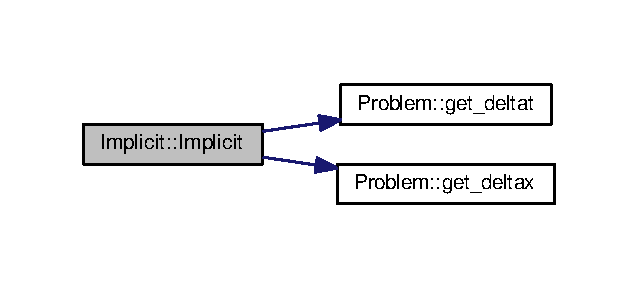
\includegraphics[width=306pt]{classImplicit_a5bc81959cd5329526f1c2b7e6e050050_cgraph}
\end{center}
\end{figure}




\subsection{Member Function Documentation}
\index{Implicit@{Implicit}!build\+\_\+r@{build\+\_\+r}}
\index{build\+\_\+r@{build\+\_\+r}!Implicit@{Implicit}}
\subsubsection[{\texorpdfstring{build\+\_\+r(\+Vector previous\+\_\+step)=0}{build_r(Vector previous_step)=0}}]{\setlength{\rightskip}{0pt plus 5cm}virtual {\bf Vector} Implicit\+::build\+\_\+r (
\begin{DoxyParamCaption}
\item[{{\bf Vector}}]{previous\+\_\+step}
\end{DoxyParamCaption}
)\hspace{0.3cm}{\ttfamily [protected]}, {\ttfamily [pure virtual]}}\hypertarget{classImplicit_ab2d07b5185008b2c845a31a03350d98d}{}\label{classImplicit_ab2d07b5185008b2c845a31a03350d98d}


A pure virtual member. 

Build the r vector in a linear system of A.\+x = r in which A is a matrix, whereas b and r are vectors. ~\newline
 This method is used to compute a solution using the thomas algorithm, which can be used in a triadiogonal matrix. 
\begin{DoxyParams}{Parameters}
{\em previous\+\_\+step} & A vector containing the previous time step solution. \\
\hline
\end{DoxyParams}
\begin{DoxyReturn}{Returns}
\hyperlink{classVector}{Vector}. The r vector, which can be used in to calculate the current time step solution with Tomas Algorithm. 
\end{DoxyReturn}


Implemented in \hyperlink{classCrankNicolson_a9b67095f05b0ee96701d6cd38099f6c4}{Crank\+Nicolson}, and \hyperlink{classLaasonen_a42cacb85b9ed27ff013a79ee2b4d923d}{Laasonen}.



Here is the caller graph for this function\+:
\nopagebreak
\begin{figure}[H]
\begin{center}
\leavevmode
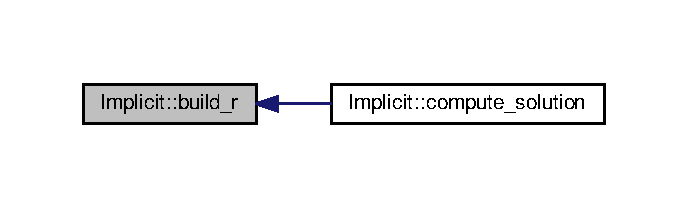
\includegraphics[width=330pt]{classImplicit_ab2d07b5185008b2c845a31a03350d98d_icgraph}
\end{center}
\end{figure}


\index{Implicit@{Implicit}!compute\+\_\+solution@{compute\+\_\+solution}}
\index{compute\+\_\+solution@{compute\+\_\+solution}!Implicit@{Implicit}}
\subsubsection[{\texorpdfstring{compute\+\_\+solution()}{compute_solution()}}]{\setlength{\rightskip}{0pt plus 5cm}void Implicit\+::compute\+\_\+solution (
\begin{DoxyParamCaption}
{}
\end{DoxyParamCaption}
)\hspace{0.3cm}{\ttfamily [virtual]}}\hypertarget{classImplicit_a1d6b7250da6d3a417baefe7328635d45}{}\label{classImplicit_a1d6b7250da6d3a417baefe7328635d45}


Normal public method. 

Calculates a solution for the given problem by populating the solution grid with the correct values. 

Implements \hyperlink{classMethod_af3dcec8e066214e82d8b4578a4a55076}{Method}.



Here is the call graph for this function\+:
\nopagebreak
\begin{figure}[H]
\begin{center}
\leavevmode
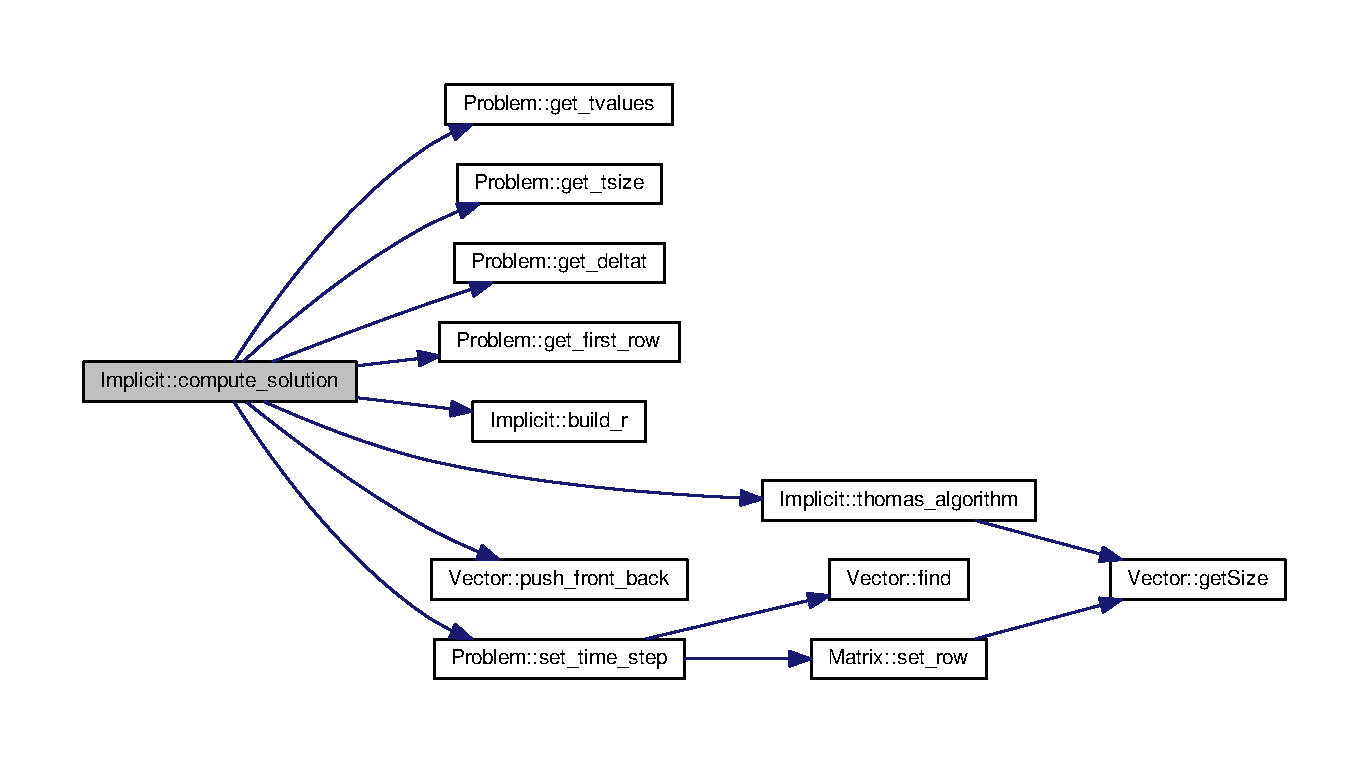
\includegraphics[width=350pt]{classImplicit_a1d6b7250da6d3a417baefe7328635d45_cgraph}
\end{center}
\end{figure}


\index{Implicit@{Implicit}!thomas\+\_\+algorithm@{thomas\+\_\+algorithm}}
\index{thomas\+\_\+algorithm@{thomas\+\_\+algorithm}!Implicit@{Implicit}}
\subsubsection[{\texorpdfstring{thomas\+\_\+algorithm(\+Vector r, double a, double b, double c)}{thomas_algorithm(Vector r, double a, double b, double c)}}]{\setlength{\rightskip}{0pt plus 5cm}{\bf Vector} Implicit\+::thomas\+\_\+algorithm (
\begin{DoxyParamCaption}
\item[{{\bf Vector}}]{r, }
\item[{double}]{a, }
\item[{double}]{b, }
\item[{double}]{c}
\end{DoxyParamCaption}
)\hspace{0.3cm}{\ttfamily [private]}}\hypertarget{classImplicit_a095e8555a718b53ff94770a0a220dfba}{}\label{classImplicit_a095e8555a718b53ff94770a0a220dfba}


Normal private method. 

Calculates the current time step with Tomas Algorithm. Giving the A.\+x = r, in which A is a matrix, whereas b and r are vectors, it calculates the b vector, since A and b are known variables. \begin{DoxySeeAlso}{See also}
\hyperlink{classImplicit_ab2d07b5185008b2c845a31a03350d98d}{build\+\_\+r(\+Vector previous\+\_\+step)} 
\end{DoxySeeAlso}

\begin{DoxyParams}{Parameters}
{\em r} & \hyperlink{classVector}{Vector} calculated by the build\+\_\+r method. \\
\hline
{\em a} & Lower diagonal value of the tridiagonal matrix \\
\hline
{\em b} & Center diagonal value of the tridiagonal matrix \\
\hline
{\em c} & Upper diagonal value of the tridiagonal matrix \\
\hline
\end{DoxyParams}
\begin{DoxyReturn}{Returns}
\hyperlink{classVector}{Vector}. \hyperlink{classVector}{Vector} that represents the current time step solution. 
\end{DoxyReturn}


Here is the call graph for this function\+:
\nopagebreak
\begin{figure}[H]
\begin{center}
\leavevmode
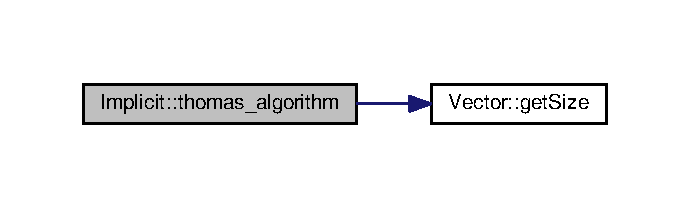
\includegraphics[width=331pt]{classImplicit_a095e8555a718b53ff94770a0a220dfba_cgraph}
\end{center}
\end{figure}




Here is the caller graph for this function\+:
\nopagebreak
\begin{figure}[H]
\begin{center}
\leavevmode
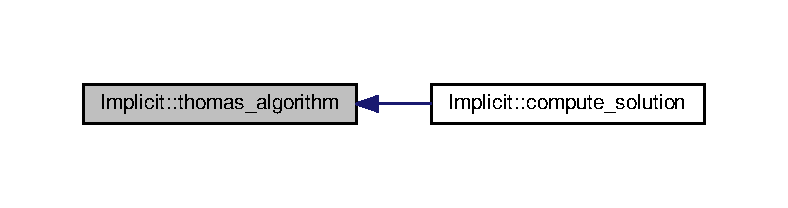
\includegraphics[width=350pt]{classImplicit_a095e8555a718b53ff94770a0a220dfba_icgraph}
\end{center}
\end{figure}




The documentation for this class was generated from the following files\+:\begin{DoxyCompactItemize}
\item 
methods/implicit/\hyperlink{implicit_8h}{implicit.\+h}\item 
methods/implicit/\hyperlink{implicit_8cpp}{implicit.\+cpp}\end{DoxyCompactItemize}

\hypertarget{classIOManager}{}\section{I\+O\+Manager Class Reference}
\label{classIOManager}\index{I\+O\+Manager@{I\+O\+Manager}}


An input/output manager class to handle plot exportations and future implementations of input handling.  




{\ttfamily \#include $<$iomanager.\+h$>$}



Collaboration diagram for I\+O\+Manager\+:
\nopagebreak
\begin{figure}[H]
\begin{center}
\leavevmode
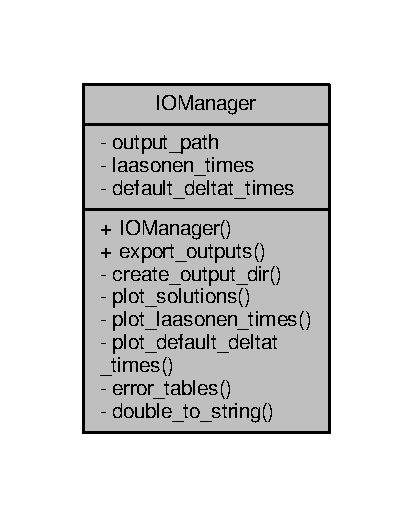
\includegraphics[width=198pt]{classIOManager__coll__graph}
\end{center}
\end{figure}
\subsection*{Public Member Functions}
\begin{DoxyCompactItemize}
\item 
\hyperlink{classIOManager_afce14d2f016545728fee1e48b74f431c}{I\+O\+Manager} ()
\begin{DoxyCompactList}\small\item\em Default constructor. \end{DoxyCompactList}\item 
void \hyperlink{classIOManager_ac4c42d2c5d93f7031447be7845bf2036}{export\+\_\+outputs} (\hyperlink{classMethod}{Method} $\ast$analytical, std\+::vector$<$ \hyperlink{classMethod}{Method} $\ast$ $>$ methods)
\begin{DoxyCompactList}\small\item\em Exports outputs regarding plots images and error tables for each computed solution, comparing them to the analytical solution. \end{DoxyCompactList}\end{DoxyCompactItemize}
\subsection*{Private Member Functions}
\begin{DoxyCompactItemize}
\item 
bool \hyperlink{classIOManager_a9798220ef88ebb14ffd354a04351862d}{create\+\_\+output\+\_\+dir} ()
\begin{DoxyCompactList}\small\item\em \hyperlink{classMethod}{Method} to create ouput folder if the folder does not exist. \end{DoxyCompactList}\item 
void \hyperlink{classIOManager_a149183e073e33890810fe6801bc4861f}{plot\+\_\+solutions} (std\+::string output\+\_\+name, \hyperlink{classMethod}{Method} $\ast$analytical, \hyperlink{classMethod}{Method} $\ast$method)
\begin{DoxyCompactList}\small\item\em Exports a plot chart that compares the analytical solution to any other solution using gnuplot. \end{DoxyCompactList}\item 
void \hyperlink{classIOManager_addf56e894f0331609d821bd515887f84}{plot\+\_\+laasonen\+\_\+times} ()
\begin{DoxyCompactList}\small\item\em Exports a plot with \hyperlink{classLaasonen}{Laasonen} delta t variation computational times. \end{DoxyCompactList}\item 
void \hyperlink{classIOManager_a12b636be3c0bab9b90ed042f450ebe8d}{plot\+\_\+default\+\_\+deltat\+\_\+times} ()
\begin{DoxyCompactList}\small\item\em Exports a plot with four methods computational times. \end{DoxyCompactList}\item 
void \hyperlink{classIOManager_a32ba797e6d5cbd6f0f8d3856b62848a2}{error\+\_\+tables} (std\+::string output\+\_\+name, std\+::vector$<$ \hyperlink{classMethod}{Method} $\ast$ $>$ method)
\begin{DoxyCompactList}\small\item\em Exports a plot that compares the norms of each solution. \end{DoxyCompactList}\item 
std\+::string \hyperlink{classIOManager_ac0848cdaa155421cd6904650823bdc9e}{double\+\_\+to\+\_\+string} (int precision, double value)
\begin{DoxyCompactList}\small\item\em Converts a double to a string with a precison of 2 decimal places. \end{DoxyCompactList}\end{DoxyCompactItemize}
\subsection*{Private Attributes}
\begin{DoxyCompactItemize}
\item 
std\+::string \hyperlink{classIOManager_a6af8948f7b74b4d6187baca2719cf8dc}{output\+\_\+path}
\begin{DoxyCompactList}\small\item\em Private string output\+\_\+path. \end{DoxyCompactList}\item 
std\+::vector$<$ double $>$ \hyperlink{classIOManager_a55739efc2d1c63b7b0c0afe2db6b294b}{laasonen\+\_\+times}
\begin{DoxyCompactList}\small\item\em Private \hyperlink{classVector}{Vector} laasonen\+\_\+times. \end{DoxyCompactList}\item 
std\+::vector$<$ double $>$ \hyperlink{classIOManager_a30696a7aaed227e80b3bbac567943eb0}{default\+\_\+deltat\+\_\+times}
\begin{DoxyCompactList}\small\item\em Private \hyperlink{classVector}{Vector} default\+\_\+deltat\+\_\+times. \end{DoxyCompactList}\end{DoxyCompactItemize}


\subsection{Detailed Description}
An input/output manager class to handle plot exportations and future implementations of input handling. 

The \hyperlink{classIOManager}{I\+O\+Manager} class provides\+: ~\newline
-\/plot method which compares the analytical solution with a set of given methods, ploting them with a custom configuration using gnuplot 

\subsection{Constructor \& Destructor Documentation}
\index{I\+O\+Manager@{I\+O\+Manager}!I\+O\+Manager@{I\+O\+Manager}}
\index{I\+O\+Manager@{I\+O\+Manager}!I\+O\+Manager@{I\+O\+Manager}}
\subsubsection[{\texorpdfstring{I\+O\+Manager()}{IOManager()}}]{\setlength{\rightskip}{0pt plus 5cm}I\+O\+Manager\+::\+I\+O\+Manager (
\begin{DoxyParamCaption}
{}
\end{DoxyParamCaption}
)}\hypertarget{classIOManager_afce14d2f016545728fee1e48b74f431c}{}\label{classIOManager_afce14d2f016545728fee1e48b74f431c}


Default constructor. 

Initialize an \hyperlink{classIOManager}{I\+O\+Manager} object. 

\subsection{Member Function Documentation}
\index{I\+O\+Manager@{I\+O\+Manager}!create\+\_\+output\+\_\+dir@{create\+\_\+output\+\_\+dir}}
\index{create\+\_\+output\+\_\+dir@{create\+\_\+output\+\_\+dir}!I\+O\+Manager@{I\+O\+Manager}}
\subsubsection[{\texorpdfstring{create\+\_\+output\+\_\+dir()}{create_output_dir()}}]{\setlength{\rightskip}{0pt plus 5cm}bool I\+O\+Manager\+::create\+\_\+output\+\_\+dir (
\begin{DoxyParamCaption}
{}
\end{DoxyParamCaption}
)\hspace{0.3cm}{\ttfamily [private]}}\hypertarget{classIOManager_a9798220ef88ebb14ffd354a04351862d}{}\label{classIOManager_a9798220ef88ebb14ffd354a04351862d}


\hyperlink{classMethod}{Method} to create ouput folder if the folder does not exist. 

\begin{DoxyReturn}{Returns}
bool. true if successfull, false if not 
\end{DoxyReturn}


Here is the caller graph for this function\+:
\nopagebreak
\begin{figure}[H]
\begin{center}
\leavevmode
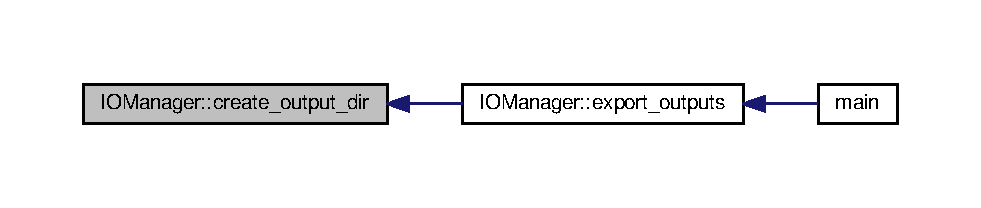
\includegraphics[width=350pt]{classIOManager_a9798220ef88ebb14ffd354a04351862d_icgraph}
\end{center}
\end{figure}


\index{I\+O\+Manager@{I\+O\+Manager}!double\+\_\+to\+\_\+string@{double\+\_\+to\+\_\+string}}
\index{double\+\_\+to\+\_\+string@{double\+\_\+to\+\_\+string}!I\+O\+Manager@{I\+O\+Manager}}
\subsubsection[{\texorpdfstring{double\+\_\+to\+\_\+string(int precision, double value)}{double_to_string(int precision, double value)}}]{\setlength{\rightskip}{0pt plus 5cm}std\+::string I\+O\+Manager\+::double\+\_\+to\+\_\+string (
\begin{DoxyParamCaption}
\item[{int}]{precision, }
\item[{double}]{value}
\end{DoxyParamCaption}
)\hspace{0.3cm}{\ttfamily [private]}}\hypertarget{classIOManager_ac0848cdaa155421cd6904650823bdc9e}{}\label{classIOManager_ac0848cdaa155421cd6904650823bdc9e}


Converts a double to a string with a precison of 2 decimal places. 


\begin{DoxyParams}{Parameters}
{\em double} & value Number to be converted \\
\hline
{\em int} & precision Precision to have \\
\hline
\end{DoxyParams}
\begin{DoxyReturn}{Returns}
string. String containing the converted number 
\end{DoxyReturn}


Here is the caller graph for this function\+:
\nopagebreak
\begin{figure}[H]
\begin{center}
\leavevmode
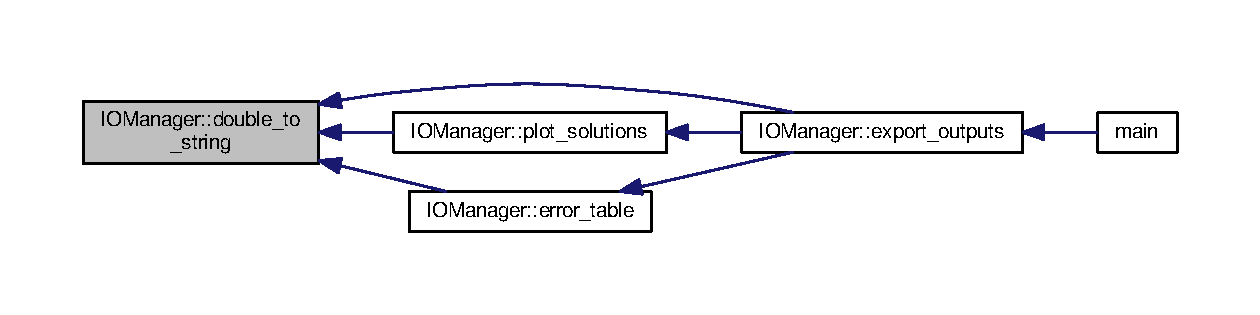
\includegraphics[width=350pt]{classIOManager_ac0848cdaa155421cd6904650823bdc9e_icgraph}
\end{center}
\end{figure}


\index{I\+O\+Manager@{I\+O\+Manager}!error\+\_\+tables@{error\+\_\+tables}}
\index{error\+\_\+tables@{error\+\_\+tables}!I\+O\+Manager@{I\+O\+Manager}}
\subsubsection[{\texorpdfstring{error\+\_\+tables(std\+::string output\+\_\+name, std\+::vector$<$ Method $\ast$ $>$ method)}{error_tables(std::string output_name, std::vector< Method * > method)}}]{\setlength{\rightskip}{0pt plus 5cm}void I\+O\+Manager\+::error\+\_\+tables (
\begin{DoxyParamCaption}
\item[{std\+::string}]{output\+\_\+name, }
\item[{std\+::vector$<$ {\bf Method} $\ast$ $>$}]{method}
\end{DoxyParamCaption}
)\hspace{0.3cm}{\ttfamily [private]}}\hypertarget{classIOManager_a32ba797e6d5cbd6f0f8d3856b62848a2}{}\label{classIOManager_a32ba797e6d5cbd6f0f8d3856b62848a2}


Exports a plot that compares the norms of each solution. 


\begin{DoxyParams}{Parameters}
{\em string} & output\+\_\+name File name to be exported \\
\hline
{\em vector$<$\+Method$\ast$$>$} & vector of methods to plot the second norm \\
\hline
\end{DoxyParams}


Here is the caller graph for this function\+:
\nopagebreak
\begin{figure}[H]
\begin{center}
\leavevmode
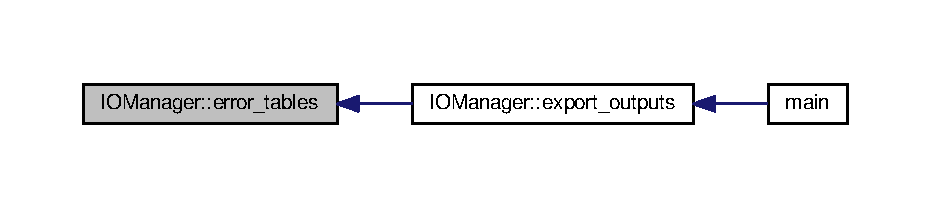
\includegraphics[width=350pt]{classIOManager_a32ba797e6d5cbd6f0f8d3856b62848a2_icgraph}
\end{center}
\end{figure}


\index{I\+O\+Manager@{I\+O\+Manager}!export\+\_\+outputs@{export\+\_\+outputs}}
\index{export\+\_\+outputs@{export\+\_\+outputs}!I\+O\+Manager@{I\+O\+Manager}}
\subsubsection[{\texorpdfstring{export\+\_\+outputs(\+Method $\ast$analytical, std\+::vector$<$ Method $\ast$ $>$ methods)}{export_outputs(Method *analytical, std::vector< Method * > methods)}}]{\setlength{\rightskip}{0pt plus 5cm}void I\+O\+Manager\+::export\+\_\+outputs (
\begin{DoxyParamCaption}
\item[{{\bf Method} $\ast$}]{analytical, }
\item[{std\+::vector$<$ {\bf Method} $\ast$ $>$}]{methods}
\end{DoxyParamCaption}
)}\hypertarget{classIOManager_ac4c42d2c5d93f7031447be7845bf2036}{}\label{classIOManager_ac4c42d2c5d93f7031447be7845bf2036}


Exports outputs regarding plots images and error tables for each computed solution, comparing them to the analytical solution. 


\begin{DoxyParams}{Parameters}
{\em Method$\ast$} & analytical The analytical solution \\
\hline
{\em vector$<$\+Method$\ast$$>$} & methods \hyperlink{classVector}{Vector} containing the solutions \\
\hline
\end{DoxyParams}


Here is the call graph for this function\+:
\nopagebreak
\begin{figure}[H]
\begin{center}
\leavevmode
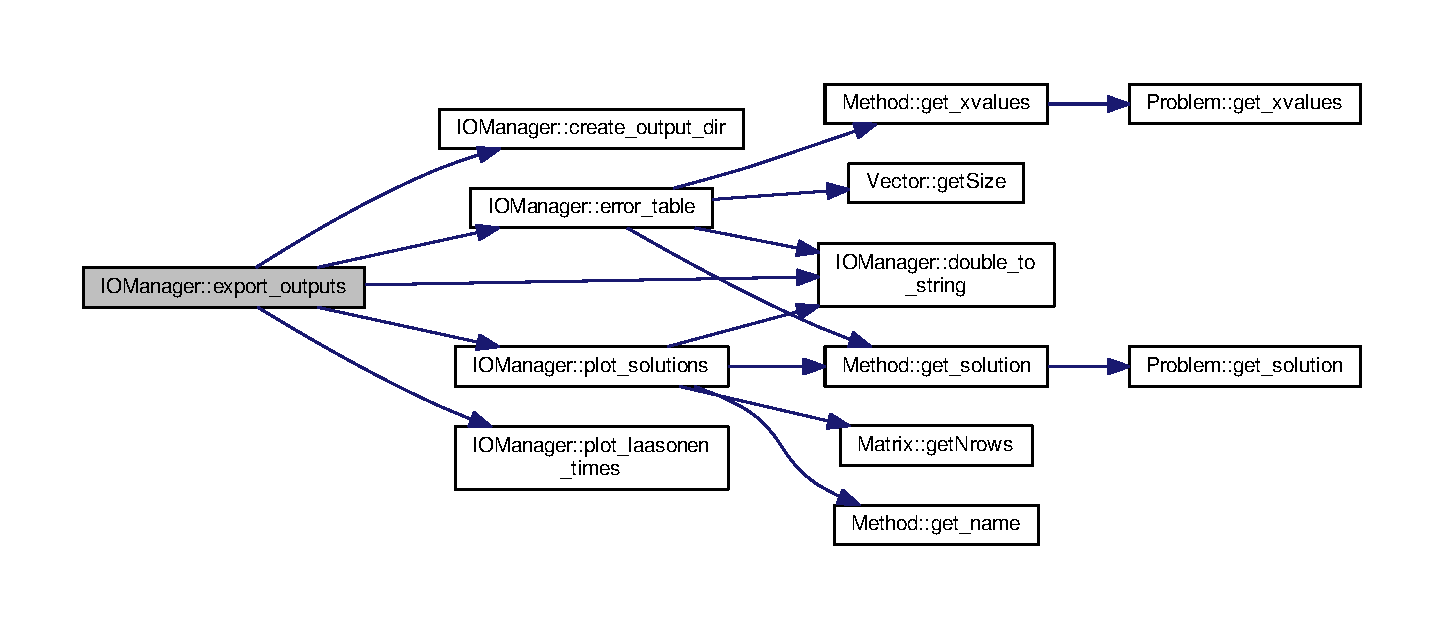
\includegraphics[width=350pt]{classIOManager_ac4c42d2c5d93f7031447be7845bf2036_cgraph}
\end{center}
\end{figure}




Here is the caller graph for this function\+:
\nopagebreak
\begin{figure}[H]
\begin{center}
\leavevmode
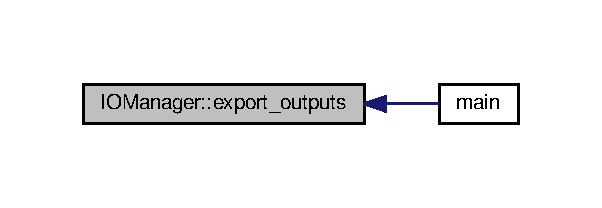
\includegraphics[width=289pt]{classIOManager_ac4c42d2c5d93f7031447be7845bf2036_icgraph}
\end{center}
\end{figure}


\index{I\+O\+Manager@{I\+O\+Manager}!plot\+\_\+default\+\_\+deltat\+\_\+times@{plot\+\_\+default\+\_\+deltat\+\_\+times}}
\index{plot\+\_\+default\+\_\+deltat\+\_\+times@{plot\+\_\+default\+\_\+deltat\+\_\+times}!I\+O\+Manager@{I\+O\+Manager}}
\subsubsection[{\texorpdfstring{plot\+\_\+default\+\_\+deltat\+\_\+times()}{plot_default_deltat_times()}}]{\setlength{\rightskip}{0pt plus 5cm}void I\+O\+Manager\+::plot\+\_\+default\+\_\+deltat\+\_\+times (
\begin{DoxyParamCaption}
{}
\end{DoxyParamCaption}
)\hspace{0.3cm}{\ttfamily [private]}}\hypertarget{classIOManager_a12b636be3c0bab9b90ed042f450ebe8d}{}\label{classIOManager_a12b636be3c0bab9b90ed042f450ebe8d}


Exports a plot with four methods computational times. 



Here is the caller graph for this function\+:
\nopagebreak
\begin{figure}[H]
\begin{center}
\leavevmode
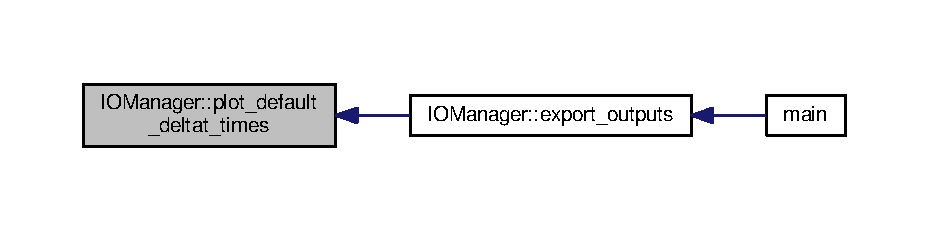
\includegraphics[width=350pt]{classIOManager_a12b636be3c0bab9b90ed042f450ebe8d_icgraph}
\end{center}
\end{figure}


\index{I\+O\+Manager@{I\+O\+Manager}!plot\+\_\+laasonen\+\_\+times@{plot\+\_\+laasonen\+\_\+times}}
\index{plot\+\_\+laasonen\+\_\+times@{plot\+\_\+laasonen\+\_\+times}!I\+O\+Manager@{I\+O\+Manager}}
\subsubsection[{\texorpdfstring{plot\+\_\+laasonen\+\_\+times()}{plot_laasonen_times()}}]{\setlength{\rightskip}{0pt plus 5cm}void I\+O\+Manager\+::plot\+\_\+laasonen\+\_\+times (
\begin{DoxyParamCaption}
{}
\end{DoxyParamCaption}
)\hspace{0.3cm}{\ttfamily [private]}}\hypertarget{classIOManager_addf56e894f0331609d821bd515887f84}{}\label{classIOManager_addf56e894f0331609d821bd515887f84}


Exports a plot with \hyperlink{classLaasonen}{Laasonen} delta t variation computational times. 



Here is the caller graph for this function\+:
\nopagebreak
\begin{figure}[H]
\begin{center}
\leavevmode
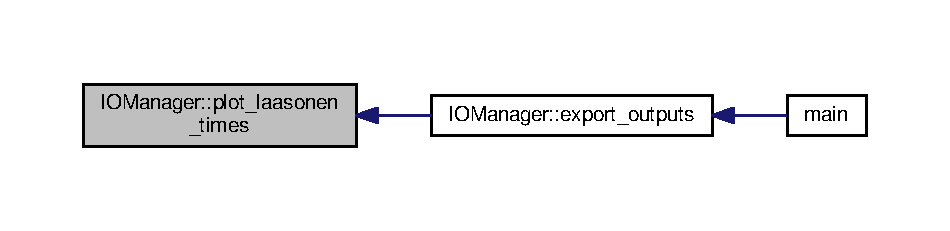
\includegraphics[width=350pt]{classIOManager_addf56e894f0331609d821bd515887f84_icgraph}
\end{center}
\end{figure}


\index{I\+O\+Manager@{I\+O\+Manager}!plot\+\_\+solutions@{plot\+\_\+solutions}}
\index{plot\+\_\+solutions@{plot\+\_\+solutions}!I\+O\+Manager@{I\+O\+Manager}}
\subsubsection[{\texorpdfstring{plot\+\_\+solutions(std\+::string output\+\_\+name, Method $\ast$analytical, Method $\ast$method)}{plot_solutions(std::string output_name, Method *analytical, Method *method)}}]{\setlength{\rightskip}{0pt plus 5cm}void I\+O\+Manager\+::plot\+\_\+solutions (
\begin{DoxyParamCaption}
\item[{std\+::string}]{output\+\_\+name, }
\item[{{\bf Method} $\ast$}]{analytical, }
\item[{{\bf Method} $\ast$}]{method}
\end{DoxyParamCaption}
)\hspace{0.3cm}{\ttfamily [private]}}\hypertarget{classIOManager_a149183e073e33890810fe6801bc4861f}{}\label{classIOManager_a149183e073e33890810fe6801bc4861f}


Exports a plot chart that compares the analytical solution to any other solution using gnuplot. 


\begin{DoxyParams}{Parameters}
{\em string} & output\+\_\+name File name to be exported \\
\hline
{\em Method$\ast$} & analytical The analytical solution \\
\hline
{\em Method$\ast$} & method Any method solution \\
\hline
\end{DoxyParams}


Here is the call graph for this function\+:
\nopagebreak
\begin{figure}[H]
\begin{center}
\leavevmode
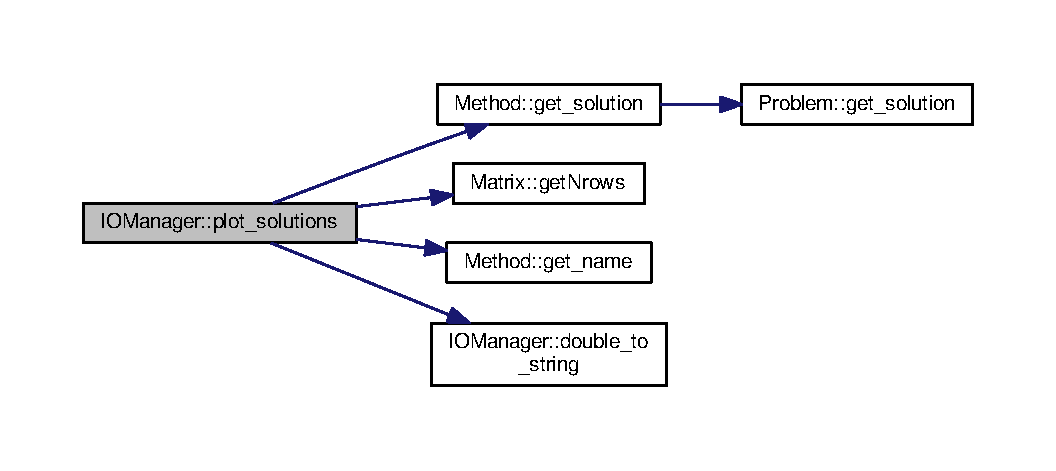
\includegraphics[width=350pt]{classIOManager_a149183e073e33890810fe6801bc4861f_cgraph}
\end{center}
\end{figure}




Here is the caller graph for this function\+:
\nopagebreak
\begin{figure}[H]
\begin{center}
\leavevmode
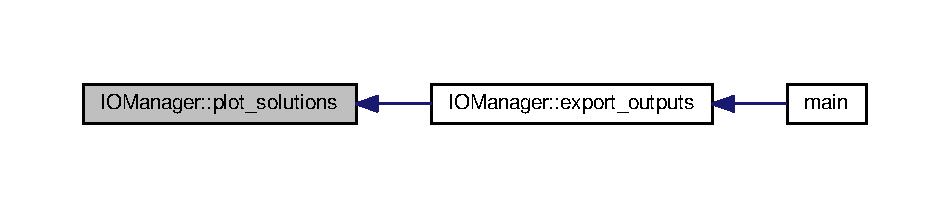
\includegraphics[width=350pt]{classIOManager_a149183e073e33890810fe6801bc4861f_icgraph}
\end{center}
\end{figure}




\subsection{Member Data Documentation}
\index{I\+O\+Manager@{I\+O\+Manager}!default\+\_\+deltat\+\_\+times@{default\+\_\+deltat\+\_\+times}}
\index{default\+\_\+deltat\+\_\+times@{default\+\_\+deltat\+\_\+times}!I\+O\+Manager@{I\+O\+Manager}}
\subsubsection[{\texorpdfstring{default\+\_\+deltat\+\_\+times}{default_deltat_times}}]{\setlength{\rightskip}{0pt plus 5cm}std\+::vector$<$double$>$ I\+O\+Manager\+::default\+\_\+deltat\+\_\+times\hspace{0.3cm}{\ttfamily [private]}}\hypertarget{classIOManager_a30696a7aaed227e80b3bbac567943eb0}{}\label{classIOManager_a30696a7aaed227e80b3bbac567943eb0}


Private \hyperlink{classVector}{Vector} default\+\_\+deltat\+\_\+times. 

Contains the computation time of each method solution, with a time step of 0.\+01. \index{I\+O\+Manager@{I\+O\+Manager}!laasonen\+\_\+times@{laasonen\+\_\+times}}
\index{laasonen\+\_\+times@{laasonen\+\_\+times}!I\+O\+Manager@{I\+O\+Manager}}
\subsubsection[{\texorpdfstring{laasonen\+\_\+times}{laasonen_times}}]{\setlength{\rightskip}{0pt plus 5cm}std\+::vector$<$double$>$ I\+O\+Manager\+::laasonen\+\_\+times\hspace{0.3cm}{\ttfamily [private]}}\hypertarget{classIOManager_a55739efc2d1c63b7b0c0afe2db6b294b}{}\label{classIOManager_a55739efc2d1c63b7b0c0afe2db6b294b}


Private \hyperlink{classVector}{Vector} laasonen\+\_\+times. 

Contains the computation time of each laasonen solution, with a different time step. \index{I\+O\+Manager@{I\+O\+Manager}!output\+\_\+path@{output\+\_\+path}}
\index{output\+\_\+path@{output\+\_\+path}!I\+O\+Manager@{I\+O\+Manager}}
\subsubsection[{\texorpdfstring{output\+\_\+path}{output_path}}]{\setlength{\rightskip}{0pt plus 5cm}std\+::string I\+O\+Manager\+::output\+\_\+path\hspace{0.3cm}{\ttfamily [private]}}\hypertarget{classIOManager_a6af8948f7b74b4d6187baca2719cf8dc}{}\label{classIOManager_a6af8948f7b74b4d6187baca2719cf8dc}


Private string output\+\_\+path. 

Contains the ouput directory path name. 

The documentation for this class was generated from the following files\+:\begin{DoxyCompactItemize}
\item 
io/\hyperlink{iomanager_8h}{iomanager.\+h}\item 
io/\hyperlink{iomanager_8cpp}{iomanager.\+cpp}\end{DoxyCompactItemize}

\hypertarget{classLaasonen}{}\section{Laasonen Class Reference}
\label{classLaasonen}\index{Laasonen@{Laasonen}}


A \hyperlink{classLaasonen}{Laasonen} method class that contains a r vector builder.  




{\ttfamily \#include $<$laasonen.\+h$>$}



Inheritance diagram for Laasonen\+:
\nopagebreak
\begin{figure}[H]
\begin{center}
\leavevmode
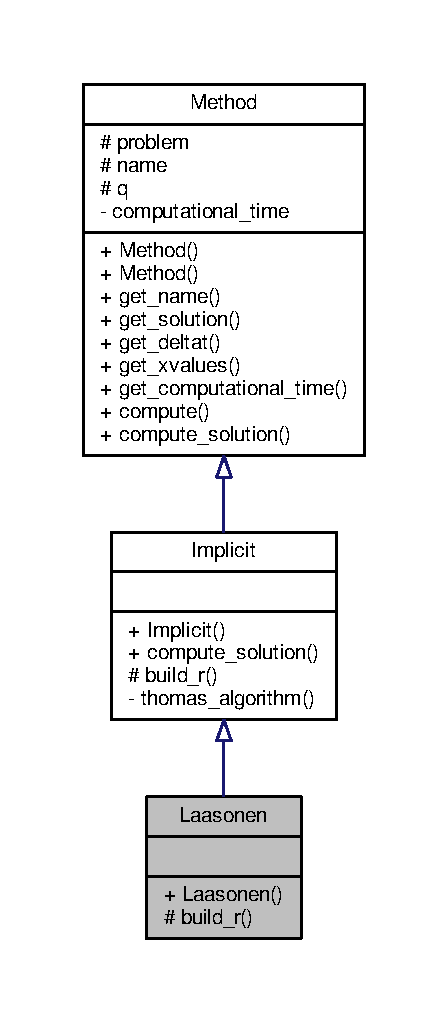
\includegraphics[width=215pt]{classLaasonen__inherit__graph}
\end{center}
\end{figure}


Collaboration diagram for Laasonen\+:
\nopagebreak
\begin{figure}[H]
\begin{center}
\leavevmode
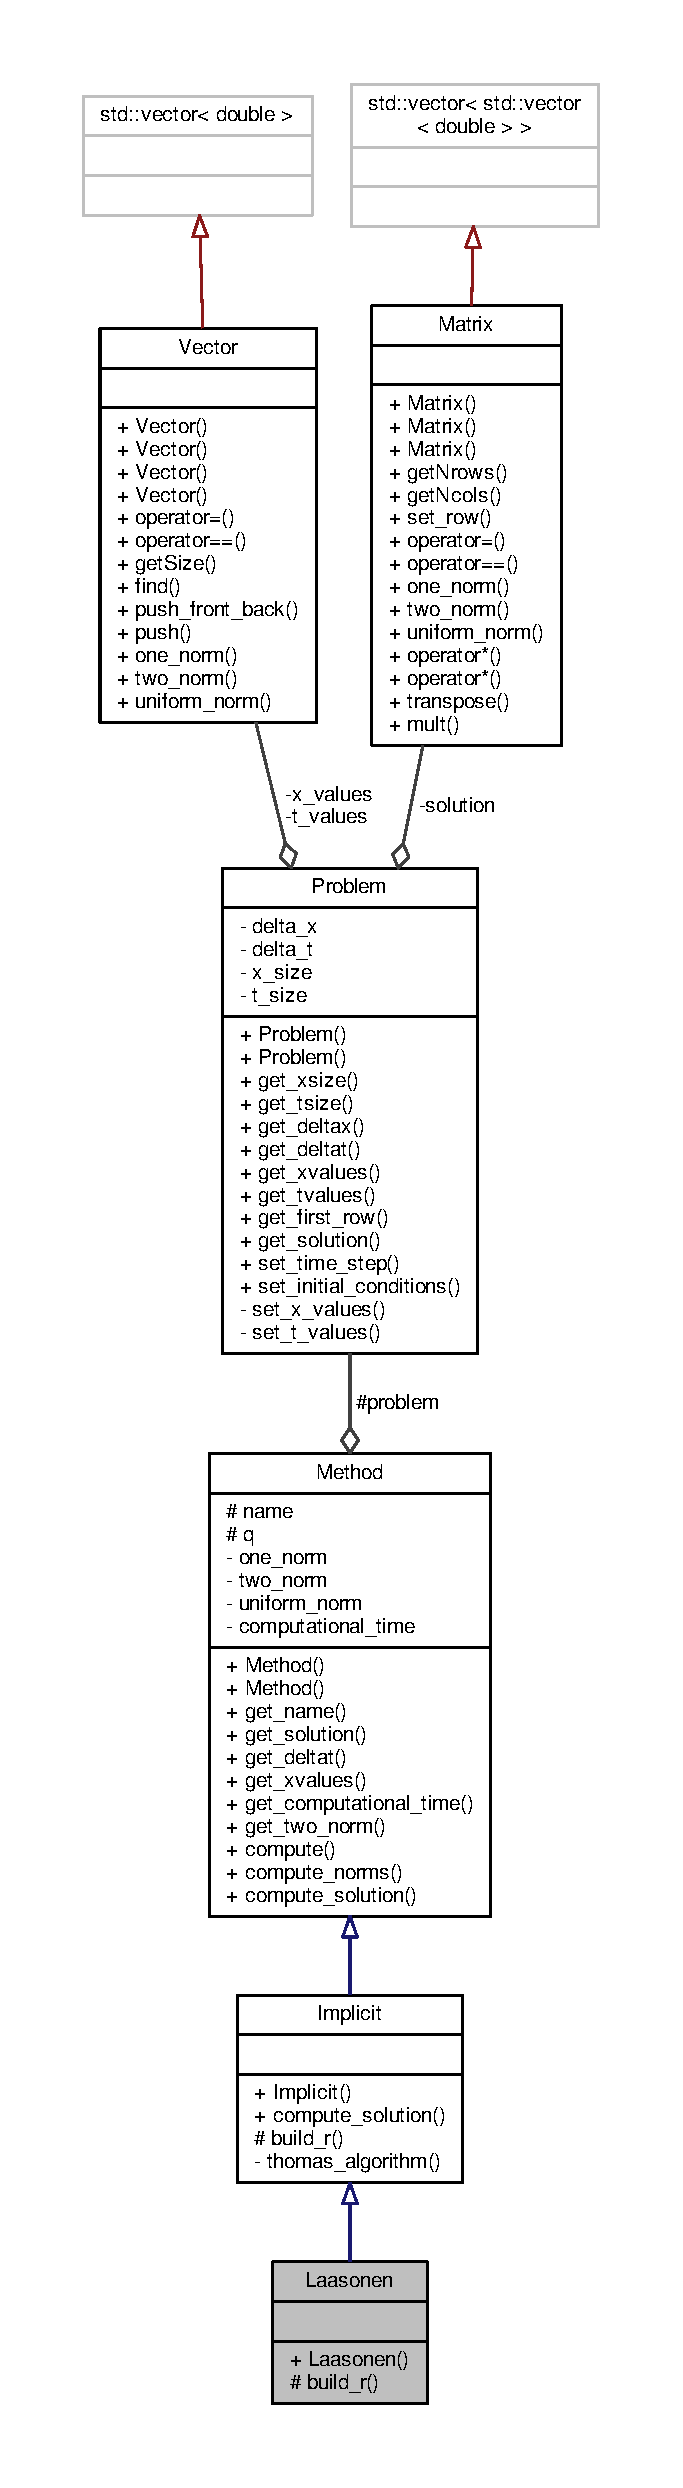
\includegraphics[height=550pt]{classLaasonen__coll__graph}
\end{center}
\end{figure}
\subsection*{Public Member Functions}
\begin{DoxyCompactItemize}
\item 
\hyperlink{classLaasonen_a1ed879786dc74b8c2ba86a1deb167e5a}{Laasonen} (\hyperlink{classProblem}{Problem} \hyperlink{classMethod_a29a08a679b5d30a8c813766308205041}{problem})
\begin{DoxyCompactList}\small\item\em Default constructor. \end{DoxyCompactList}\end{DoxyCompactItemize}
\subsection*{Protected Member Functions}
\begin{DoxyCompactItemize}
\item 
\hyperlink{classVector}{Vector} \hyperlink{classLaasonen_a42cacb85b9ed27ff013a79ee2b4d923d}{build\+\_\+r} (\hyperlink{classVector}{Vector} previous\+\_\+step)
\begin{DoxyCompactList}\small\item\em Normal protected method. \end{DoxyCompactList}\end{DoxyCompactItemize}
\subsection*{Additional Inherited Members}


\subsection{Detailed Description}
A \hyperlink{classLaasonen}{Laasonen} method class that contains a r vector builder. 

~\newline
 This builder is used is used to calculate the r vector in A.\+x = r linear equation system.

The \hyperlink{classLaasonen}{Laasonen} class provides\+: ~\newline
-\/a basic constructor for creating a \hyperlink{classLaasonen}{Laasonen} method object. ~\newline
-\/a method to compute the r vector. 

\subsection{Constructor \& Destructor Documentation}
\index{Laasonen@{Laasonen}!Laasonen@{Laasonen}}
\index{Laasonen@{Laasonen}!Laasonen@{Laasonen}}
\subsubsection[{\texorpdfstring{Laasonen(\+Problem problem)}{Laasonen(Problem problem)}}]{\setlength{\rightskip}{0pt plus 5cm}Laasonen\+::\+Laasonen (
\begin{DoxyParamCaption}
\item[{{\bf Problem}}]{problem}
\end{DoxyParamCaption}
)}\hypertarget{classLaasonen_a1ed879786dc74b8c2ba86a1deb167e5a}{}\label{classLaasonen_a1ed879786dc74b8c2ba86a1deb167e5a}


Default constructor. 



\subsection{Member Function Documentation}
\index{Laasonen@{Laasonen}!build\+\_\+r@{build\+\_\+r}}
\index{build\+\_\+r@{build\+\_\+r}!Laasonen@{Laasonen}}
\subsubsection[{\texorpdfstring{build\+\_\+r(\+Vector previous\+\_\+step)}{build_r(Vector previous_step)}}]{\setlength{\rightskip}{0pt plus 5cm}{\bf Vector} Laasonen\+::build\+\_\+r (
\begin{DoxyParamCaption}
\item[{{\bf Vector}}]{previous\+\_\+step}
\end{DoxyParamCaption}
)\hspace{0.3cm}{\ttfamily [protected]}, {\ttfamily [virtual]}}\hypertarget{classLaasonen_a42cacb85b9ed27ff013a79ee2b4d923d}{}\label{classLaasonen_a42cacb85b9ed27ff013a79ee2b4d923d}


Normal protected method. 

get the number of rows 
\begin{DoxyParams}{Parameters}
{\em previous\+\_\+step} & \hyperlink{classVector}{Vector} representing the solution of the previous time step. \\
\hline
\end{DoxyParams}
\begin{DoxyReturn}{Returns}
\hyperlink{classVector}{Vector}. r vector to be used in A.\+x = r 
\end{DoxyReturn}


Implements \hyperlink{classImplicit_ab2d07b5185008b2c845a31a03350d98d}{Implicit}.



Here is the call graph for this function\+:
\nopagebreak
\begin{figure}[H]
\begin{center}
\leavevmode
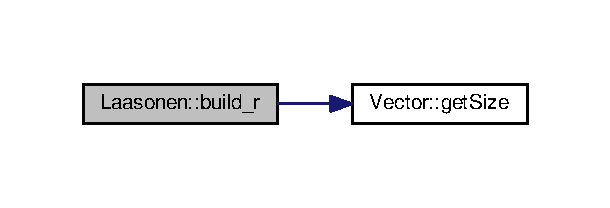
\includegraphics[width=293pt]{classLaasonen_a42cacb85b9ed27ff013a79ee2b4d923d_cgraph}
\end{center}
\end{figure}




The documentation for this class was generated from the following files\+:\begin{DoxyCompactItemize}
\item 
methods/implicit/\hyperlink{laasonen_8h}{laasonen.\+h}\item 
methods/implicit/\hyperlink{laasonen_8cpp}{laasonen.\+cpp}\end{DoxyCompactItemize}

\hypertarget{classMatrix}{}\section{Matrix Class Reference}
\label{classMatrix}\index{Matrix@{Matrix}}


A matrix class for data storage of a 2D array of doubles ~\newline
 The implementation is derived from the standard container vector std\+::vector ~\newline
 We use private inheritance to base our vector upon the library version whilst  usto expose only those base class functions we wish to use -\/ in this  the array access operator \mbox{[}\mbox{]}.  




{\ttfamily \#include $<$matrix.\+h$>$}



Inheritance diagram for Matrix\+:
\nopagebreak
\begin{figure}[H]
\begin{center}
\leavevmode
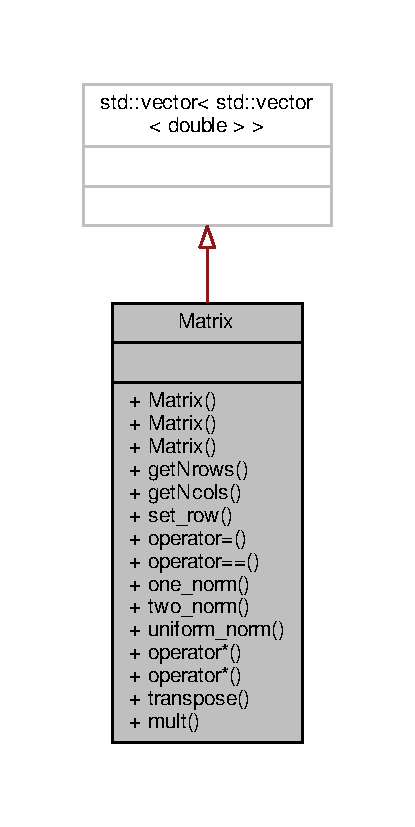
\includegraphics[width=199pt]{classMatrix__inherit__graph}
\end{center}
\end{figure}


Collaboration diagram for Matrix\+:
\nopagebreak
\begin{figure}[H]
\begin{center}
\leavevmode
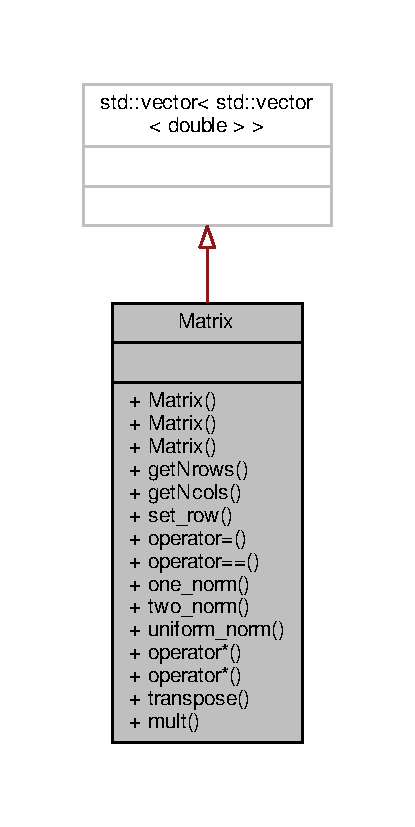
\includegraphics[width=199pt]{classMatrix__coll__graph}
\end{center}
\end{figure}
\subsection*{Public Member Functions}
\begin{DoxyCompactItemize}
\item 
\hyperlink{classMatrix_a2dba13c45127354c9f75ef576f49269b}{Matrix} ()
\begin{DoxyCompactList}\small\item\em Default constructor. \end{DoxyCompactList}\item 
\hyperlink{classMatrix_a135a15de1126d735bb95fcc839d739d7}{Matrix} (int Nrows, int Ncols)
\begin{DoxyCompactList}\small\item\em Alternate constructor. \end{DoxyCompactList}\item 
\hyperlink{classMatrix_a765f4dcb51b6829311cc3e7576388423}{Matrix} (const \hyperlink{classMatrix}{Matrix} \&m)
\begin{DoxyCompactList}\small\item\em Copy constructor. \end{DoxyCompactList}\item 
int \hyperlink{classMatrix_ab0ed1933348c0511d74f825b73778aaa}{get\+Nrows} () const 
\begin{DoxyCompactList}\small\item\em Normal public get method. \end{DoxyCompactList}\item 
int \hyperlink{classMatrix_a09f35c4f255ad102a8692a4a2c6ccc0d}{get\+Ncols} () const 
\begin{DoxyCompactList}\small\item\em Normal public get method. \end{DoxyCompactList}\item 
void \hyperlink{classMatrix_a24066c6e9743a07387bcb287437a6cea}{set\+\_\+row} (int index, \hyperlink{classVector}{Vector} v)
\begin{DoxyCompactList}\small\item\em Normal public set method. \end{DoxyCompactList}\item 
\hyperlink{classMatrix}{Matrix} \& \hyperlink{classMatrix_aea5a06385f646eb4a63929fae6fa3e14}{operator=} (const \hyperlink{classMatrix}{Matrix} \&m)
\begin{DoxyCompactList}\small\item\em Overloaded assignment operator. \end{DoxyCompactList}\item 
bool \hyperlink{classMatrix_a5bc97450e589f9ae3a43814808645f3f}{operator==} (const \hyperlink{classMatrix}{Matrix} \&m) const 
\begin{DoxyCompactList}\small\item\em Overloaded comparison operator returns true or false depending on whether the matrices are the same or not. \end{DoxyCompactList}\item 
double \hyperlink{classMatrix_a4f7ede695709b614f2e1f6423a024201}{one\+\_\+norm} () const 
\begin{DoxyCompactList}\small\item\em Normal public method that returns a double. \end{DoxyCompactList}\item 
double \hyperlink{classMatrix_a0b738b2c1d87ec28b23c7e479d014f2a}{two\+\_\+norm} () const 
\begin{DoxyCompactList}\small\item\em Normal public method that returns a double. \end{DoxyCompactList}\item 
double \hyperlink{classMatrix_a05777a670e901010b96e9d667a4bdd3b}{uniform\+\_\+norm} () const 
\begin{DoxyCompactList}\small\item\em Normal public method that returns a double. \end{DoxyCompactList}\item 
\hyperlink{classMatrix}{Matrix} \hyperlink{classMatrix_a1fbef471bec2714e891c082a345d2274}{operator$\ast$} (const \hyperlink{classMatrix}{Matrix} \&a) const 
\begin{DoxyCompactList}\small\item\em Overloaded $\ast$operator that returns a \hyperlink{classMatrix}{Matrix}. \end{DoxyCompactList}\item 
\hyperlink{classVector}{Vector} \hyperlink{classMatrix_a31aaaadc4c2f30ce01cd70c2e0c72f6f}{operator$\ast$} (const \hyperlink{classVector}{Vector} \&v) const 
\begin{DoxyCompactList}\small\item\em Overloaded $\ast$operator that returns a \hyperlink{classVector}{Vector}. \end{DoxyCompactList}\item 
\hyperlink{classMatrix}{Matrix} \hyperlink{classMatrix_a9da9f5ee8215491cc54ecc59ddeb3f73}{transpose} () const 
\begin{DoxyCompactList}\small\item\em public method that returns the transpose of the matrix. \end{DoxyCompactList}\item 
\hyperlink{classMatrix}{Matrix} \hyperlink{classMatrix_a28ac82d2f9ec7e4f8a366ec7bd6bd54e}{mult} (const \hyperlink{classMatrix}{Matrix} \&a) const 
\end{DoxyCompactItemize}
\subsection*{Private Types}
\begin{DoxyCompactItemize}
\item 
typedef std\+::vector$<$ std\+::vector$<$ double $>$ $>$ \hyperlink{classMatrix_a0027109b5516f852be28259267c6c637}{vec}
\end{DoxyCompactItemize}
\subsection*{Friends}
\begin{DoxyCompactItemize}
\item 
std\+::istream \& \hyperlink{classMatrix_a3d6c1dcfc038804f4c08687f4f37f48b}{operator$>$$>$} (std\+::istream \&is, \hyperlink{classMatrix}{Matrix} \&m)
\begin{DoxyCompactList}\small\item\em Overloaded istream $>$$>$ operator. \end{DoxyCompactList}\item 
std\+::ostream \& \hyperlink{classMatrix_a060711074cb5bcaf4e75498bc040c4b7}{operator$<$$<$} (std\+::ostream \&os, const \hyperlink{classMatrix}{Matrix} \&m)
\begin{DoxyCompactList}\small\item\em Overloaded ostream $<$$<$ operator. \end{DoxyCompactList}\item 
std\+::ifstream \& \hyperlink{classMatrix_aa5699a0bdf0ee014f083ff8a76629d21}{operator$>$$>$} (std\+::ifstream \&ifs, \hyperlink{classMatrix}{Matrix} \&m)
\begin{DoxyCompactList}\small\item\em Overloaded ifstream $>$$>$ operator. \end{DoxyCompactList}\item 
std\+::ofstream \& \hyperlink{classMatrix_aa574249d63b390cf1108d6e82047ef61}{operator$<$$<$} (std\+::ofstream \&ofs, const \hyperlink{classMatrix}{Matrix} \&m)
\begin{DoxyCompactList}\small\item\em Overloaded ofstream $<$$<$ operator. \end{DoxyCompactList}\end{DoxyCompactItemize}


\subsection{Detailed Description}
A matrix class for data storage of a 2D array of doubles ~\newline
 The implementation is derived from the standard container vector std\+::vector ~\newline
 We use private inheritance to base our vector upon the library version whilst  usto expose only those base class functions we wish to use -\/ in this  the array access operator \mbox{[}\mbox{]}. 

The \hyperlink{classMatrix}{Matrix} class provides\+: ~\newline
-\/basic constructors for creating a matrix object from other matrix object,  by creating empty matrix of a given size, ~\newline
-\/input and oput operation via $>$$>$ and $<$$<$ operators using keyboard or file ~\newline
-\/basic operations like access via \mbox{[}\mbox{]} operator, assignment and comparision 

\subsection{Member Typedef Documentation}
\index{Matrix@{Matrix}!vec@{vec}}
\index{vec@{vec}!Matrix@{Matrix}}
\subsubsection[{\texorpdfstring{vec}{vec}}]{\setlength{\rightskip}{0pt plus 5cm}typedef std\+::vector$<$std\+::vector$<$double$>$ $>$ {\bf Matrix\+::vec}\hspace{0.3cm}{\ttfamily [private]}}\hypertarget{classMatrix_a0027109b5516f852be28259267c6c637}{}\label{classMatrix_a0027109b5516f852be28259267c6c637}


\subsection{Constructor \& Destructor Documentation}
\index{Matrix@{Matrix}!Matrix@{Matrix}}
\index{Matrix@{Matrix}!Matrix@{Matrix}}
\subsubsection[{\texorpdfstring{Matrix()}{Matrix()}}]{\setlength{\rightskip}{0pt plus 5cm}Matrix\+::\+Matrix (
\begin{DoxyParamCaption}
{}
\end{DoxyParamCaption}
)}\hypertarget{classMatrix_a2dba13c45127354c9f75ef576f49269b}{}\label{classMatrix_a2dba13c45127354c9f75ef576f49269b}


Default constructor. 

Intialize an empty \hyperlink{classMatrix}{Matrix} object \begin{DoxySeeAlso}{See also}
\hyperlink{classMatrix_a135a15de1126d735bb95fcc839d739d7}{Matrix(int Nrows, int Ncols)} 

\hyperlink{classMatrix_a765f4dcb51b6829311cc3e7576388423}{Matrix(const Matrix\& m)} 
\end{DoxySeeAlso}


Here is the caller graph for this function\+:
\nopagebreak
\begin{figure}[H]
\begin{center}
\leavevmode
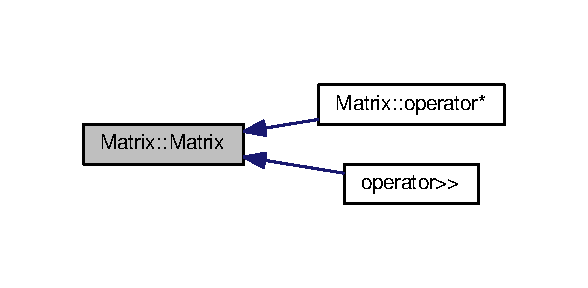
\includegraphics[width=282pt]{classMatrix_a2dba13c45127354c9f75ef576f49269b_icgraph}
\end{center}
\end{figure}


\index{Matrix@{Matrix}!Matrix@{Matrix}}
\index{Matrix@{Matrix}!Matrix@{Matrix}}
\subsubsection[{\texorpdfstring{Matrix(int Nrows, int Ncols)}{Matrix(int Nrows, int Ncols)}}]{\setlength{\rightskip}{0pt plus 5cm}Matrix\+::\+Matrix (
\begin{DoxyParamCaption}
\item[{int}]{Nrows, }
\item[{int}]{Ncols}
\end{DoxyParamCaption}
)}\hypertarget{classMatrix_a135a15de1126d735bb95fcc839d739d7}{}\label{classMatrix_a135a15de1126d735bb95fcc839d739d7}


Alternate constructor. 

build a matrix Nrows by Ncols \begin{DoxySeeAlso}{See also}
\hyperlink{classMatrix_a2dba13c45127354c9f75ef576f49269b}{Matrix()} 

\hyperlink{classMatrix_a765f4dcb51b6829311cc3e7576388423}{Matrix(const Matrix\& m)} 
\end{DoxySeeAlso}

\begin{DoxyExceptions}{Exceptions}
{\em invalid\+\_\+argument} & (\char`\"{}matrix size negative or zero\char`\"{}) \\
\hline
\end{DoxyExceptions}

\begin{DoxyParams}{Parameters}
{\em Nrows} & int. number of rows in matrix \\
\hline
{\em Ncols} & int. number of columns in matrix \\
\hline
\end{DoxyParams}
\index{Matrix@{Matrix}!Matrix@{Matrix}}
\index{Matrix@{Matrix}!Matrix@{Matrix}}
\subsubsection[{\texorpdfstring{Matrix(const Matrix \&m)}{Matrix(const Matrix &m)}}]{\setlength{\rightskip}{0pt plus 5cm}Matrix\+::\+Matrix (
\begin{DoxyParamCaption}
\item[{const {\bf Matrix} \&}]{m}
\end{DoxyParamCaption}
)}\hypertarget{classMatrix_a765f4dcb51b6829311cc3e7576388423}{}\label{classMatrix_a765f4dcb51b6829311cc3e7576388423}


Copy constructor. 

build a matrix from another matrix \begin{DoxySeeAlso}{See also}
\hyperlink{classMatrix_a2dba13c45127354c9f75ef576f49269b}{Matrix()} 

\hyperlink{classMatrix_a135a15de1126d735bb95fcc839d739d7}{Matrix(int Nrows, int Ncols)} 
\end{DoxySeeAlso}

\begin{DoxyParams}{Parameters}
{\em m} & \hyperlink{classMatrix}{Matrix}\&. matrix to copy from \\
\hline
\end{DoxyParams}


Here is the call graph for this function\+:
\nopagebreak
\begin{figure}[H]
\begin{center}
\leavevmode
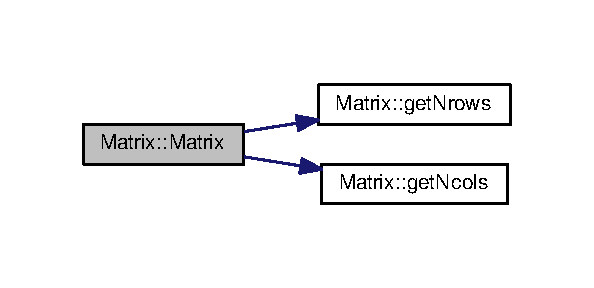
\includegraphics[width=285pt]{classMatrix_a765f4dcb51b6829311cc3e7576388423_cgraph}
\end{center}
\end{figure}




\subsection{Member Function Documentation}
\index{Matrix@{Matrix}!get\+Ncols@{get\+Ncols}}
\index{get\+Ncols@{get\+Ncols}!Matrix@{Matrix}}
\subsubsection[{\texorpdfstring{get\+Ncols() const }{getNcols() const }}]{\setlength{\rightskip}{0pt plus 5cm}int Matrix\+::get\+Ncols (
\begin{DoxyParamCaption}
{}
\end{DoxyParamCaption}
) const}\hypertarget{classMatrix_a09f35c4f255ad102a8692a4a2c6ccc0d}{}\label{classMatrix_a09f35c4f255ad102a8692a4a2c6ccc0d}


Normal public get method. 

get the number of columns \begin{DoxySeeAlso}{See also}
int \hyperlink{classMatrix_ab0ed1933348c0511d74f825b73778aaa}{get\+Nrows()const} 
\end{DoxySeeAlso}
\begin{DoxyReturn}{Returns}
int. number of columns in matrix 
\end{DoxyReturn}


Here is the caller graph for this function\+:
\nopagebreak
\begin{figure}[H]
\begin{center}
\leavevmode
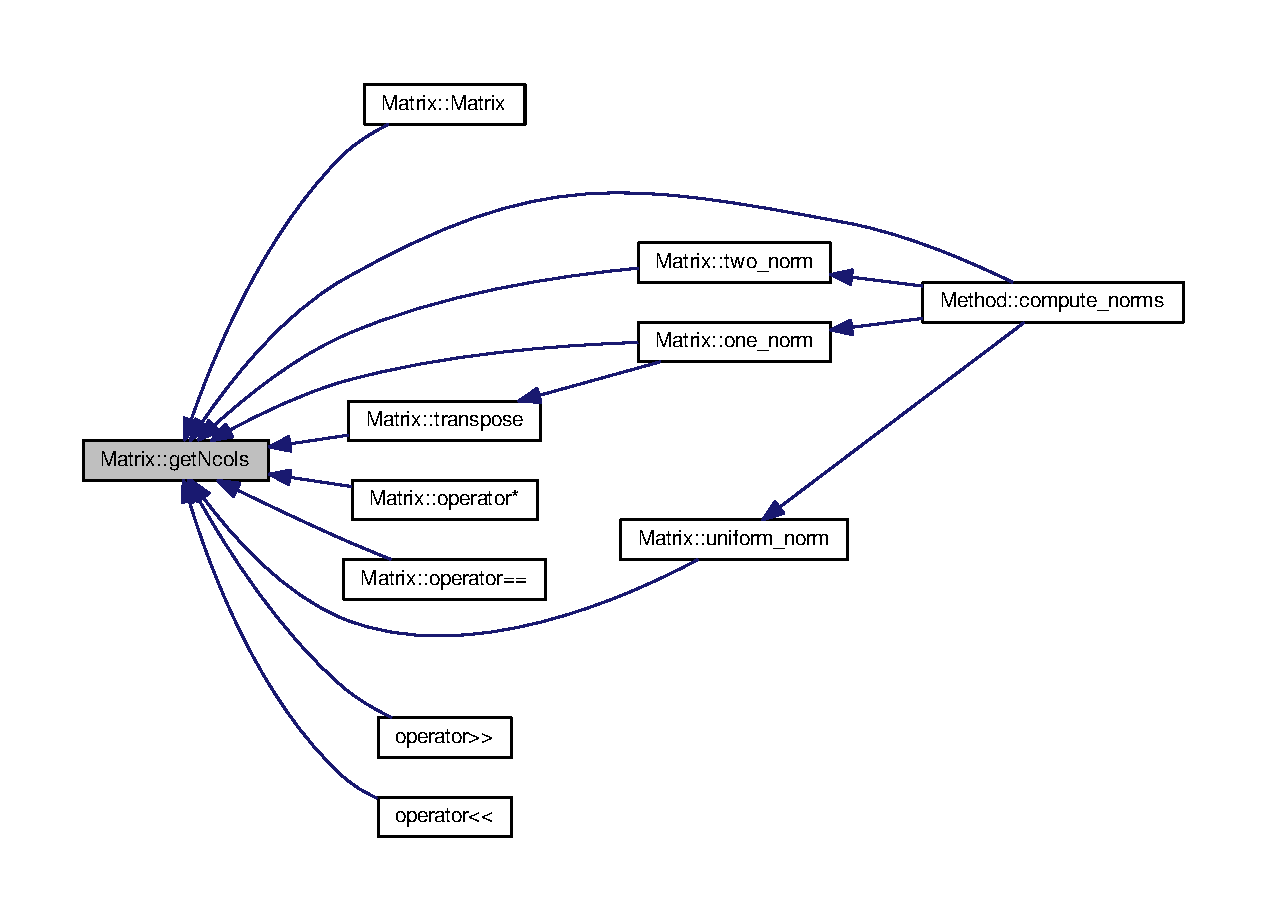
\includegraphics[width=350pt]{classMatrix_a09f35c4f255ad102a8692a4a2c6ccc0d_icgraph}
\end{center}
\end{figure}


\index{Matrix@{Matrix}!get\+Nrows@{get\+Nrows}}
\index{get\+Nrows@{get\+Nrows}!Matrix@{Matrix}}
\subsubsection[{\texorpdfstring{get\+Nrows() const }{getNrows() const }}]{\setlength{\rightskip}{0pt plus 5cm}int Matrix\+::get\+Nrows (
\begin{DoxyParamCaption}
{}
\end{DoxyParamCaption}
) const}\hypertarget{classMatrix_ab0ed1933348c0511d74f825b73778aaa}{}\label{classMatrix_ab0ed1933348c0511d74f825b73778aaa}


Normal public get method. 

get the number of rows \begin{DoxySeeAlso}{See also}
int \hyperlink{classMatrix_a09f35c4f255ad102a8692a4a2c6ccc0d}{get\+Ncols()const} 
\end{DoxySeeAlso}
\begin{DoxyReturn}{Returns}
int. number of rows in matrix 
\end{DoxyReturn}


Here is the caller graph for this function\+:
\nopagebreak
\begin{figure}[H]
\begin{center}
\leavevmode
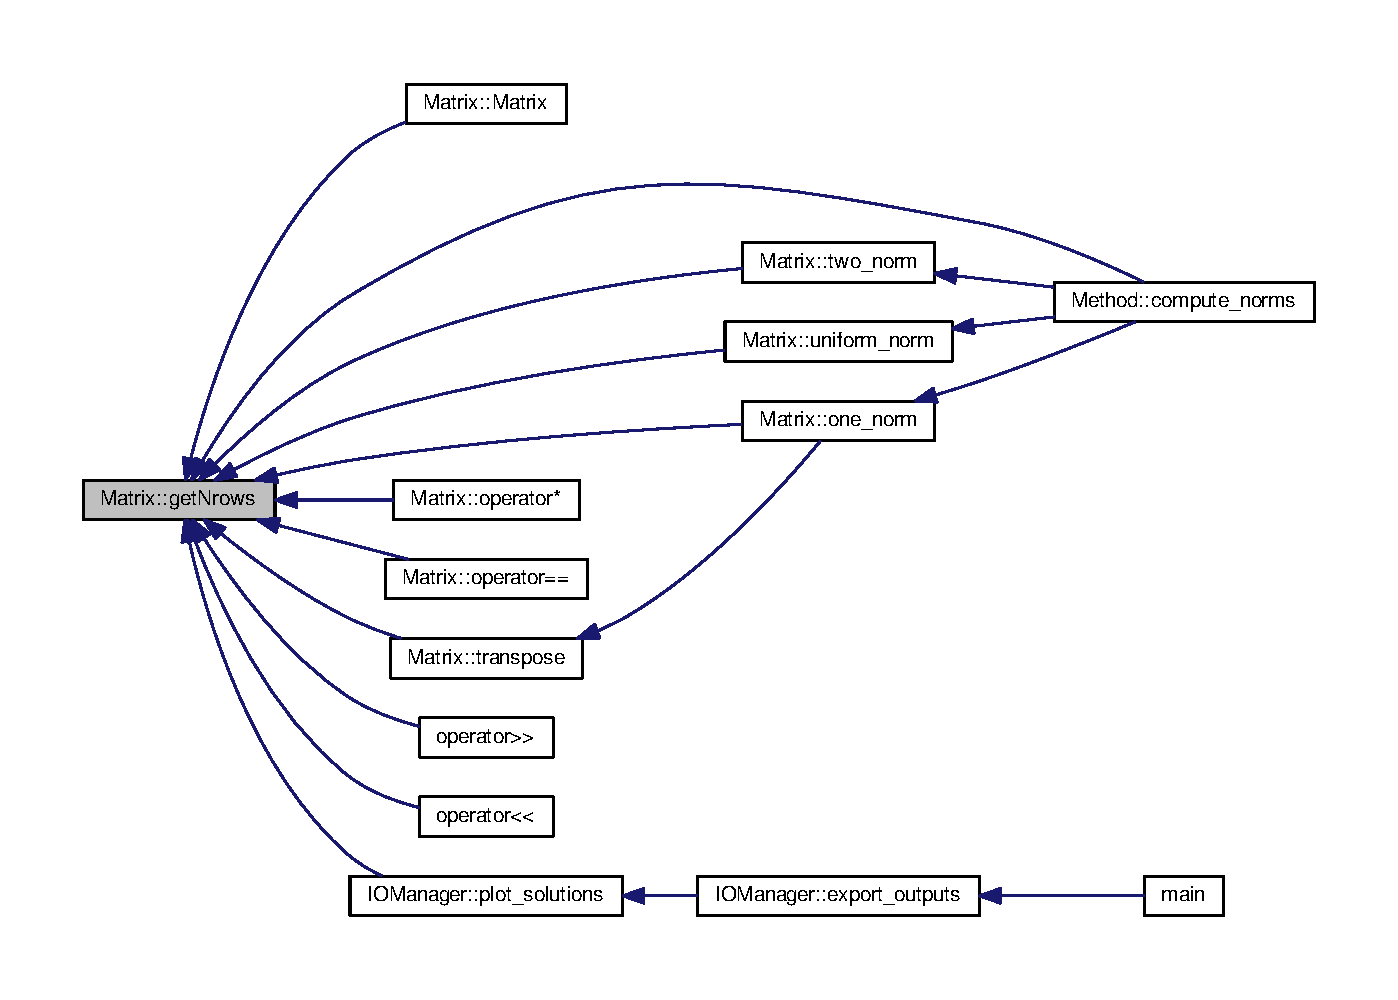
\includegraphics[width=350pt]{classMatrix_ab0ed1933348c0511d74f825b73778aaa_icgraph}
\end{center}
\end{figure}


\index{Matrix@{Matrix}!mult@{mult}}
\index{mult@{mult}!Matrix@{Matrix}}
\subsubsection[{\texorpdfstring{mult(const Matrix \&a) const }{mult(const Matrix &a) const }}]{\setlength{\rightskip}{0pt plus 5cm}{\bf Matrix} Matrix\+::mult (
\begin{DoxyParamCaption}
\item[{const {\bf Matrix} \&}]{a}
\end{DoxyParamCaption}
) const}\hypertarget{classMatrix_a28ac82d2f9ec7e4f8a366ec7bd6bd54e}{}\label{classMatrix_a28ac82d2f9ec7e4f8a366ec7bd6bd54e}
\index{Matrix@{Matrix}!one\+\_\+norm@{one\+\_\+norm}}
\index{one\+\_\+norm@{one\+\_\+norm}!Matrix@{Matrix}}
\subsubsection[{\texorpdfstring{one\+\_\+norm() const }{one_norm() const }}]{\setlength{\rightskip}{0pt plus 5cm}double Matrix\+::one\+\_\+norm (
\begin{DoxyParamCaption}
{}
\end{DoxyParamCaption}
) const}\hypertarget{classMatrix_a4f7ede695709b614f2e1f6423a024201}{}\label{classMatrix_a4f7ede695709b614f2e1f6423a024201}


Normal public method that returns a double. 

It returns L1 norm of matrix \begin{DoxySeeAlso}{See also}
\hyperlink{classMatrix_a0b738b2c1d87ec28b23c7e479d014f2a}{two\+\_\+norm()const} 

\hyperlink{classMatrix_a05777a670e901010b96e9d667a4bdd3b}{uniform\+\_\+norm()const} 
\end{DoxySeeAlso}
\begin{DoxyReturn}{Returns}
double. matrix L1 norm 
\end{DoxyReturn}


Here is the call graph for this function\+:
\nopagebreak
\begin{figure}[H]
\begin{center}
\leavevmode
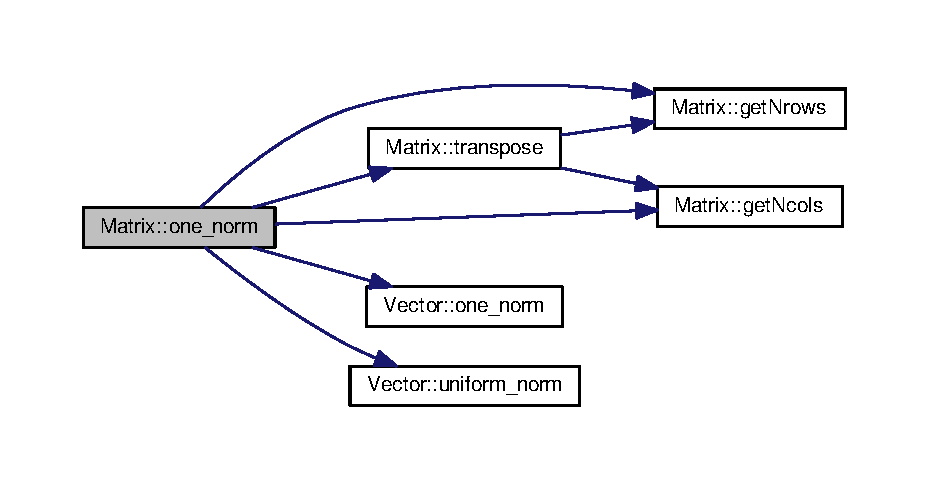
\includegraphics[width=350pt]{classMatrix_a4f7ede695709b614f2e1f6423a024201_cgraph}
\end{center}
\end{figure}




Here is the caller graph for this function\+:
\nopagebreak
\begin{figure}[H]
\begin{center}
\leavevmode
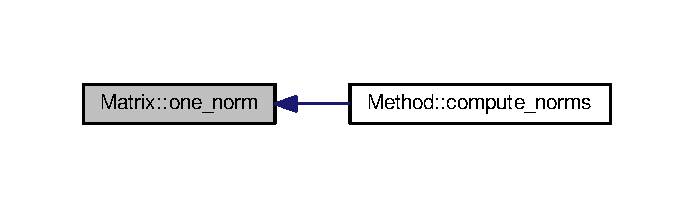
\includegraphics[width=333pt]{classMatrix_a4f7ede695709b614f2e1f6423a024201_icgraph}
\end{center}
\end{figure}


\index{Matrix@{Matrix}!operator$\ast$@{operator$\ast$}}
\index{operator$\ast$@{operator$\ast$}!Matrix@{Matrix}}
\subsubsection[{\texorpdfstring{operator$\ast$(const Matrix \&a) const }{operator*(const Matrix &a) const }}]{\setlength{\rightskip}{0pt plus 5cm}{\bf Matrix} Matrix\+::operator$\ast$ (
\begin{DoxyParamCaption}
\item[{const {\bf Matrix} \&}]{a}
\end{DoxyParamCaption}
) const}\hypertarget{classMatrix_a1fbef471bec2714e891c082a345d2274}{}\label{classMatrix_a1fbef471bec2714e891c082a345d2274}


Overloaded $\ast$operator that returns a \hyperlink{classMatrix}{Matrix}. 

It Performs matrix by matrix multiplication. \begin{DoxySeeAlso}{See also}
\hyperlink{classMatrix_a1fbef471bec2714e891c082a345d2274}{operator$\ast$(const Matrix \& a) const} 
\end{DoxySeeAlso}

\begin{DoxyExceptions}{Exceptions}
{\em out\+\_\+of\+\_\+range} & (\char`\"{}\+Matrix access error\char`\"{}) One or more of the matrix have a zero size \\
\hline
{\em std\+::out\+\_\+of\+\_\+range} & (\char`\"{}uncompatible matrix sizes\char`\"{}) Number of columns in first matrix do not match number of columns in second matrix \\
\hline
\end{DoxyExceptions}
\begin{DoxyReturn}{Returns}
\hyperlink{classMatrix}{Matrix}. matrix-\/matrix product 
\end{DoxyReturn}

\begin{DoxyParams}{Parameters}
{\em a} & \hyperlink{classMatrix}{Matrix}. matrix to multiply by \\
\hline
\end{DoxyParams}


Here is the call graph for this function\+:
\nopagebreak
\begin{figure}[H]
\begin{center}
\leavevmode
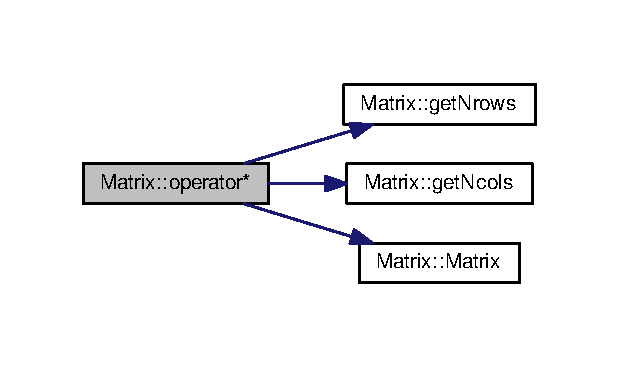
\includegraphics[width=297pt]{classMatrix_a1fbef471bec2714e891c082a345d2274_cgraph}
\end{center}
\end{figure}


\index{Matrix@{Matrix}!operator$\ast$@{operator$\ast$}}
\index{operator$\ast$@{operator$\ast$}!Matrix@{Matrix}}
\subsubsection[{\texorpdfstring{operator$\ast$(const Vector \&v) const }{operator*(const Vector &v) const }}]{\setlength{\rightskip}{0pt plus 5cm}{\bf Vector} Matrix\+::operator$\ast$ (
\begin{DoxyParamCaption}
\item[{const {\bf Vector} \&}]{v}
\end{DoxyParamCaption}
) const}\hypertarget{classMatrix_a31aaaadc4c2f30ce01cd70c2e0c72f6f}{}\label{classMatrix_a31aaaadc4c2f30ce01cd70c2e0c72f6f}


Overloaded $\ast$operator that returns a \hyperlink{classVector}{Vector}. 

It Performs matrix by vector multiplication. \begin{DoxySeeAlso}{See also}
\hyperlink{classMatrix_a1fbef471bec2714e891c082a345d2274}{operator$\ast$(const Matrix \& a)const} 
\end{DoxySeeAlso}

\begin{DoxyExceptions}{Exceptions}
{\em std\+::out\+\_\+of\+\_\+range} & (\char`\"{}\+Matrix access error\char`\"{}) matrix has a zero size \\
\hline
{\em std\+::out\+\_\+of\+\_\+range} & (\char`\"{}\+Vector access error\char`\"{}) vector has a zero size \\
\hline
{\em std\+::out\+\_\+of\+\_\+range} & (\char`\"{}uncompatible matrix-\/vector sizes\char`\"{}) Number of columns in matrix do not match the vector size \\
\hline
\end{DoxyExceptions}
\begin{DoxyReturn}{Returns}
\hyperlink{classVector}{Vector}. matrix-\/vector product 
\end{DoxyReturn}

\begin{DoxyParams}{Parameters}
{\em v} & \hyperlink{classVector}{Vector}. \hyperlink{classVector}{Vector} to multiply by \\
\hline
\end{DoxyParams}


Here is the call graph for this function\+:
\nopagebreak
\begin{figure}[H]
\begin{center}
\leavevmode
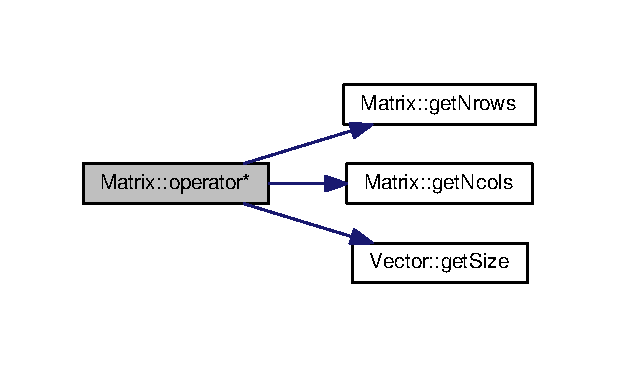
\includegraphics[width=297pt]{classMatrix_a31aaaadc4c2f30ce01cd70c2e0c72f6f_cgraph}
\end{center}
\end{figure}


\index{Matrix@{Matrix}!operator=@{operator=}}
\index{operator=@{operator=}!Matrix@{Matrix}}
\subsubsection[{\texorpdfstring{operator=(const Matrix \&m)}{operator=(const Matrix &m)}}]{\setlength{\rightskip}{0pt plus 5cm}{\bf Matrix} \& Matrix\+::operator= (
\begin{DoxyParamCaption}
\item[{const {\bf Matrix} \&}]{m}
\end{DoxyParamCaption}
)}\hypertarget{classMatrix_aea5a06385f646eb4a63929fae6fa3e14}{}\label{classMatrix_aea5a06385f646eb4a63929fae6fa3e14}


Overloaded assignment operator. 

\begin{DoxySeeAlso}{See also}
\hyperlink{classMatrix_a5bc97450e589f9ae3a43814808645f3f}{operator==(const Matrix\& m)const} 
\end{DoxySeeAlso}
\begin{DoxyReturn}{Returns}
\hyperlink{classMatrix}{Matrix}\&. the matrix on the left of the assignment 
\end{DoxyReturn}

\begin{DoxyParams}{Parameters}
{\em m} & \hyperlink{classMatrix}{Matrix}\&. \hyperlink{classMatrix}{Matrix} to assign from \\
\hline
\end{DoxyParams}
\index{Matrix@{Matrix}!operator==@{operator==}}
\index{operator==@{operator==}!Matrix@{Matrix}}
\subsubsection[{\texorpdfstring{operator==(const Matrix \&m) const }{operator==(const Matrix &m) const }}]{\setlength{\rightskip}{0pt plus 5cm}bool Matrix\+::operator== (
\begin{DoxyParamCaption}
\item[{const {\bf Matrix} \&}]{m}
\end{DoxyParamCaption}
) const}\hypertarget{classMatrix_a5bc97450e589f9ae3a43814808645f3f}{}\label{classMatrix_a5bc97450e589f9ae3a43814808645f3f}


Overloaded comparison operator returns true or false depending on whether the matrices are the same or not. 

\begin{DoxySeeAlso}{See also}
\hyperlink{classMatrix_aea5a06385f646eb4a63929fae6fa3e14}{operator=(const Matrix\& m)} 
\end{DoxySeeAlso}
\begin{DoxyReturn}{Returns}
bool. true or false 
\end{DoxyReturn}

\begin{DoxyParams}{Parameters}
{\em m} & \hyperlink{classMatrix}{Matrix}\&. \hyperlink{classMatrix}{Matrix} to compare to \\
\hline
\end{DoxyParams}


Here is the call graph for this function\+:
\nopagebreak
\begin{figure}[H]
\begin{center}
\leavevmode
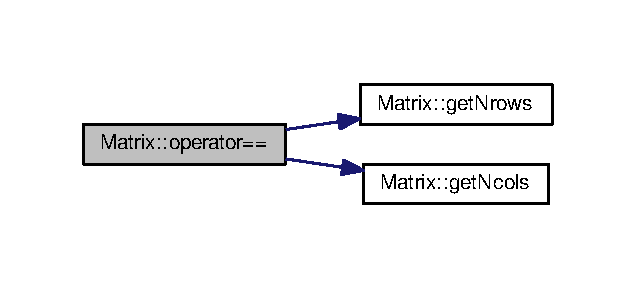
\includegraphics[width=305pt]{classMatrix_a5bc97450e589f9ae3a43814808645f3f_cgraph}
\end{center}
\end{figure}


\index{Matrix@{Matrix}!set\+\_\+row@{set\+\_\+row}}
\index{set\+\_\+row@{set\+\_\+row}!Matrix@{Matrix}}
\subsubsection[{\texorpdfstring{set\+\_\+row(int index, Vector v)}{set_row(int index, Vector v)}}]{\setlength{\rightskip}{0pt plus 5cm}void Matrix\+::set\+\_\+row (
\begin{DoxyParamCaption}
\item[{int}]{index, }
\item[{{\bf Vector}}]{v}
\end{DoxyParamCaption}
)}\hypertarget{classMatrix_a24066c6e9743a07387bcb287437a6cea}{}\label{classMatrix_a24066c6e9743a07387bcb287437a6cea}


Normal public set method. 

replace a row with a given vector 
\begin{DoxyParams}{Parameters}
{\em index} & Index of row to mutate \\
\hline
{\em v} & New vector \\
\hline
\end{DoxyParams}

\begin{DoxyExceptions}{Exceptions}
{\em out\+\_\+of\+\_\+range} & (\char`\"{}index out of range.\textbackslash{}n\char`\"{}) \\
\hline
{\em out\+\_\+of\+\_\+range} & (\char`\"{}vector size is different from matrix columns number.\textbackslash{}n\char`\"{}) \\
\hline
\end{DoxyExceptions}


Here is the call graph for this function\+:
\nopagebreak
\begin{figure}[H]
\begin{center}
\leavevmode
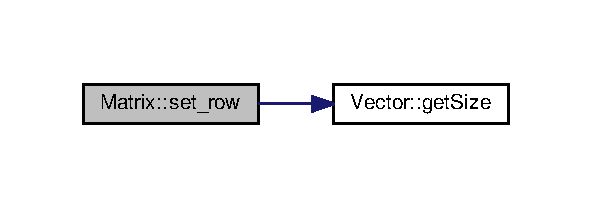
\includegraphics[width=284pt]{classMatrix_a24066c6e9743a07387bcb287437a6cea_cgraph}
\end{center}
\end{figure}




Here is the caller graph for this function\+:
\nopagebreak
\begin{figure}[H]
\begin{center}
\leavevmode
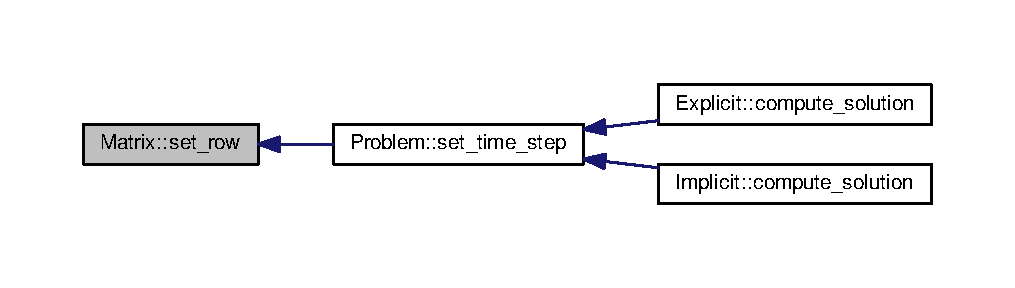
\includegraphics[width=350pt]{classMatrix_a24066c6e9743a07387bcb287437a6cea_icgraph}
\end{center}
\end{figure}


\index{Matrix@{Matrix}!transpose@{transpose}}
\index{transpose@{transpose}!Matrix@{Matrix}}
\subsubsection[{\texorpdfstring{transpose() const }{transpose() const }}]{\setlength{\rightskip}{0pt plus 5cm}{\bf Matrix} Matrix\+::transpose (
\begin{DoxyParamCaption}
{}
\end{DoxyParamCaption}
) const}\hypertarget{classMatrix_a9da9f5ee8215491cc54ecc59ddeb3f73}{}\label{classMatrix_a9da9f5ee8215491cc54ecc59ddeb3f73}


public method that returns the transpose of the matrix. 

It returns the transpose of matrix \begin{DoxyReturn}{Returns}
\hyperlink{classMatrix}{Matrix}. matrix transpose 
\end{DoxyReturn}


Here is the call graph for this function\+:
\nopagebreak
\begin{figure}[H]
\begin{center}
\leavevmode
\includegraphics[width=300pt]{classMatrix_a9da9f5ee8215491cc54ecc59ddeb3f73_cgraph}
\end{center}
\end{figure}




Here is the caller graph for this function\+:
\nopagebreak
\begin{figure}[H]
\begin{center}
\leavevmode
\includegraphics[width=350pt]{classMatrix_a9da9f5ee8215491cc54ecc59ddeb3f73_icgraph}
\end{center}
\end{figure}


\index{Matrix@{Matrix}!two\+\_\+norm@{two\+\_\+norm}}
\index{two\+\_\+norm@{two\+\_\+norm}!Matrix@{Matrix}}
\subsubsection[{\texorpdfstring{two\+\_\+norm() const }{two_norm() const }}]{\setlength{\rightskip}{0pt plus 5cm}double Matrix\+::two\+\_\+norm (
\begin{DoxyParamCaption}
{}
\end{DoxyParamCaption}
) const}\hypertarget{classMatrix_a0b738b2c1d87ec28b23c7e479d014f2a}{}\label{classMatrix_a0b738b2c1d87ec28b23c7e479d014f2a}


Normal public method that returns a double. 

It returns L2 norm of matrix \begin{DoxySeeAlso}{See also}
\hyperlink{classMatrix_a4f7ede695709b614f2e1f6423a024201}{one\+\_\+norm()const} 

\hyperlink{classMatrix_a05777a670e901010b96e9d667a4bdd3b}{uniform\+\_\+norm()const} 
\end{DoxySeeAlso}
\begin{DoxyReturn}{Returns}
double. matrix L2 norm 
\end{DoxyReturn}


Here is the call graph for this function\+:
\nopagebreak
\begin{figure}[H]
\begin{center}
\leavevmode
\includegraphics[width=300pt]{classMatrix_a0b738b2c1d87ec28b23c7e479d014f2a_cgraph}
\end{center}
\end{figure}




Here is the caller graph for this function\+:
\nopagebreak
\begin{figure}[H]
\begin{center}
\leavevmode
\includegraphics[width=333pt]{classMatrix_a0b738b2c1d87ec28b23c7e479d014f2a_icgraph}
\end{center}
\end{figure}


\index{Matrix@{Matrix}!uniform\+\_\+norm@{uniform\+\_\+norm}}
\index{uniform\+\_\+norm@{uniform\+\_\+norm}!Matrix@{Matrix}}
\subsubsection[{\texorpdfstring{uniform\+\_\+norm() const }{uniform_norm() const }}]{\setlength{\rightskip}{0pt plus 5cm}double Matrix\+::uniform\+\_\+norm (
\begin{DoxyParamCaption}
{}
\end{DoxyParamCaption}
) const}\hypertarget{classMatrix_a05777a670e901010b96e9d667a4bdd3b}{}\label{classMatrix_a05777a670e901010b96e9d667a4bdd3b}


Normal public method that returns a double. 

It returns L\+\_\+max norm of matrix \begin{DoxySeeAlso}{See also}
\hyperlink{classMatrix_a4f7ede695709b614f2e1f6423a024201}{one\+\_\+norm()const} 

\hyperlink{classMatrix_a0b738b2c1d87ec28b23c7e479d014f2a}{two\+\_\+norm()const} 
\end{DoxySeeAlso}
\begin{DoxyReturn}{Returns}
double. matrix L\+\_\+max norm 
\end{DoxyReturn}


Here is the call graph for this function\+:
\nopagebreak
\begin{figure}[H]
\begin{center}
\leavevmode
\includegraphics[width=335pt]{classMatrix_a05777a670e901010b96e9d667a4bdd3b_cgraph}
\end{center}
\end{figure}




Here is the caller graph for this function\+:
\nopagebreak
\begin{figure}[H]
\begin{center}
\leavevmode
\includegraphics[width=350pt]{classMatrix_a05777a670e901010b96e9d667a4bdd3b_icgraph}
\end{center}
\end{figure}




\subsection{Friends And Related Function Documentation}
\index{Matrix@{Matrix}!operator$<$$<$@{operator$<$$<$}}
\index{operator$<$$<$@{operator$<$$<$}!Matrix@{Matrix}}
\subsubsection[{\texorpdfstring{operator$<$$<$}{operator<<}}]{\setlength{\rightskip}{0pt plus 5cm}std\+::ostream\& operator$<$$<$ (
\begin{DoxyParamCaption}
\item[{std\+::ostream \&}]{os, }
\item[{const {\bf Matrix} \&}]{m}
\end{DoxyParamCaption}
)\hspace{0.3cm}{\ttfamily [friend]}}\hypertarget{classMatrix_a060711074cb5bcaf4e75498bc040c4b7}{}\label{classMatrix_a060711074cb5bcaf4e75498bc040c4b7}


Overloaded ostream $<$$<$ operator. 

Display output if matrix has size user will be asked to input only matrix values if matrix was not initialized user can choose matrix size and input it values \begin{DoxySeeAlso}{See also}
\hyperlink{classMatrix_aa5699a0bdf0ee014f083ff8a76629d21}{operator$>$$>$(std\+::ifstream\& ifs, Matrix\& m)} 

\hyperlink{classMatrix_a3d6c1dcfc038804f4c08687f4f37f48b}{operator$>$$>$(std\+::istream\& is, Matrix\& m)} 

\hyperlink{classMatrix_a060711074cb5bcaf4e75498bc040c4b7}{operator$<$$<$(std\+::ostream\& os, const Matrix\& m)} 
\end{DoxySeeAlso}
\begin{DoxyReturn}{Returns}
std\+::ostream\&. The ostream object 
\end{DoxyReturn}

\begin{DoxyParams}{Parameters}
{\em os} & Display output stream \\
\hline
{\em m} & \hyperlink{classMatrix}{Matrix} to read from \\
\hline
\end{DoxyParams}
\index{Matrix@{Matrix}!operator$<$$<$@{operator$<$$<$}}
\index{operator$<$$<$@{operator$<$$<$}!Matrix@{Matrix}}
\subsubsection[{\texorpdfstring{operator$<$$<$}{operator<<}}]{\setlength{\rightskip}{0pt plus 5cm}std\+::ofstream\& operator$<$$<$ (
\begin{DoxyParamCaption}
\item[{std\+::ofstream \&}]{ofs, }
\item[{const {\bf Matrix} \&}]{m}
\end{DoxyParamCaption}
)\hspace{0.3cm}{\ttfamily [friend]}}\hypertarget{classMatrix_aa574249d63b390cf1108d6e82047ef61}{}\label{classMatrix_aa574249d63b390cf1108d6e82047ef61}


Overloaded ofstream $<$$<$ operator. 

File output the file output operator is compatible with file input operator, ie. everything written can be read later. \begin{DoxySeeAlso}{See also}
\hyperlink{classMatrix_aa5699a0bdf0ee014f083ff8a76629d21}{operator$>$$>$(std\+::ifstream\& ifs, Matrix\& m)} 

\hyperlink{classMatrix_aa574249d63b390cf1108d6e82047ef61}{operator$<$$<$(std\+::ofstream\& ofs, const Matrix\& m)} 

\hyperlink{classMatrix_a3d6c1dcfc038804f4c08687f4f37f48b}{operator$>$$>$(std\+::istream\& is, Matrix\& m)} 
\end{DoxySeeAlso}

\begin{DoxyExceptions}{Exceptions}
{\em std\+::invalid\+\_\+argument} & (\char`\"{}file read error -\/ negative matrix size\char`\"{}); \\
\hline
\end{DoxyExceptions}
\begin{DoxyReturn}{Returns}
std\+::ofstream\&. The ofstream object 
\end{DoxyReturn}

\begin{DoxyParams}{Parameters}
{\em m} & \hyperlink{classMatrix}{Matrix} to read from \\
\hline
\end{DoxyParams}
\index{Matrix@{Matrix}!operator$>$$>$@{operator$>$$>$}}
\index{operator$>$$>$@{operator$>$$>$}!Matrix@{Matrix}}
\subsubsection[{\texorpdfstring{operator$>$$>$}{operator>>}}]{\setlength{\rightskip}{0pt plus 5cm}std\+::istream\& operator$>$$>$ (
\begin{DoxyParamCaption}
\item[{std\+::istream \&}]{is, }
\item[{{\bf Matrix} \&}]{m}
\end{DoxyParamCaption}
)\hspace{0.3cm}{\ttfamily [friend]}}\hypertarget{classMatrix_a3d6c1dcfc038804f4c08687f4f37f48b}{}\label{classMatrix_a3d6c1dcfc038804f4c08687f4f37f48b}


Overloaded istream $>$$>$ operator. 

Keyboard input if matrix has size user will be asked to input only matrix values if matrix was not initialized user can choose matrix size and input it values \begin{DoxySeeAlso}{See also}
\hyperlink{classMatrix_aa574249d63b390cf1108d6e82047ef61}{operator$<$$<$(std\+::ofstream\& ofs, const Matrix\& m)} 

\hyperlink{classMatrix_a3d6c1dcfc038804f4c08687f4f37f48b}{operator$>$$>$(std\+::istream\& is, Matrix\& m)} 

\hyperlink{classMatrix_a060711074cb5bcaf4e75498bc040c4b7}{operator$<$$<$(std\+::ostream\& os, const Matrix\& m)} 
\end{DoxySeeAlso}

\begin{DoxyExceptions}{Exceptions}
{\em std\+::invalid\+\_\+argument} & (\char`\"{}read error -\/ negative matrix size\char`\"{}); \\
\hline
\end{DoxyExceptions}
\begin{DoxyReturn}{Returns}
std\+::istream\&. The istream object 
\end{DoxyReturn}

\begin{DoxyParams}{Parameters}
{\em is} & Keyboard input stream \\
\hline
{\em m} & \hyperlink{classMatrix}{Matrix} to write into \\
\hline
\end{DoxyParams}
\index{Matrix@{Matrix}!operator$>$$>$@{operator$>$$>$}}
\index{operator$>$$>$@{operator$>$$>$}!Matrix@{Matrix}}
\subsubsection[{\texorpdfstring{operator$>$$>$}{operator>>}}]{\setlength{\rightskip}{0pt plus 5cm}std\+::ifstream\& operator$>$$>$ (
\begin{DoxyParamCaption}
\item[{std\+::ifstream \&}]{ifs, }
\item[{{\bf Matrix} \&}]{m}
\end{DoxyParamCaption}
)\hspace{0.3cm}{\ttfamily [friend]}}\hypertarget{classMatrix_aa5699a0bdf0ee014f083ff8a76629d21}{}\label{classMatrix_aa5699a0bdf0ee014f083ff8a76629d21}


Overloaded ifstream $>$$>$ operator. 

File input the file output operator is compatible with file input operator, ie. everything written can be read later. \begin{DoxySeeAlso}{See also}
\hyperlink{classMatrix_aa5699a0bdf0ee014f083ff8a76629d21}{operator$>$$>$(std\+::ifstream\& ifs, Matrix\& m)} 

\hyperlink{classMatrix_aa574249d63b390cf1108d6e82047ef61}{operator$<$$<$(std\+::ofstream\& ofs, const Matrix\& m)} 

\hyperlink{classMatrix_a060711074cb5bcaf4e75498bc040c4b7}{operator$<$$<$(std\+::ostream\& os, const Matrix\& m)} 
\end{DoxySeeAlso}
\begin{DoxyReturn}{Returns}
std\+::ifstream\&. The ifstream object 
\end{DoxyReturn}

\begin{DoxyParams}{Parameters}
{\em ifs} & Input file stream with opened matrix file \\
\hline
{\em m} & \hyperlink{classMatrix}{Matrix} to write into \\
\hline
\end{DoxyParams}


The documentation for this class was generated from the following files\+:\begin{DoxyCompactItemize}
\item 
grid/\hyperlink{matrix_8h}{matrix.\+h}\item 
grid/\hyperlink{matrix_8cpp}{matrix.\+cpp}\end{DoxyCompactItemize}

\hypertarget{classMethod}{}\section{Method Class Reference}
\label{classMethod}\index{Method@{Method}}


A \hyperlink{classMethod}{Method} class to structure information used to solve the problem.  




{\ttfamily \#include $<$method.\+h$>$}



Inheritance diagram for Method\+:
\nopagebreak
\begin{figure}[H]
\begin{center}
\leavevmode
\includegraphics[width=350pt]{classMethod__inherit__graph}
\end{center}
\end{figure}


Collaboration diagram for Method\+:
\nopagebreak
\begin{figure}[H]
\begin{center}
\leavevmode
\includegraphics[height=550pt]{classMethod__coll__graph}
\end{center}
\end{figure}
\subsection*{Public Member Functions}
\begin{DoxyCompactItemize}
\item 
\hyperlink{classMethod_ab48717dc68d3c057b65574a539a480f7}{Method} ()
\begin{DoxyCompactList}\small\item\em Default constructor. \end{DoxyCompactList}\item 
\hyperlink{classMethod_ad27fe6ae65cd4571d52cba8562b16222}{Method} (\hyperlink{classProblem}{Problem} \hyperlink{classMethod_a29a08a679b5d30a8c813766308205041}{problem})
\begin{DoxyCompactList}\small\item\em Alternate constructor. \end{DoxyCompactList}\item 
std\+::string \hyperlink{classMethod_a103a9b2dcf6ef35857e279ba1e5ef9c3}{get\+\_\+name} ()
\begin{DoxyCompactList}\small\item\em Normal public get method. \end{DoxyCompactList}\item 
\hyperlink{classMatrix}{Matrix} \hyperlink{classMethod_a2a10100e81e4aca97f7ef485ed11fbe6}{get\+\_\+solution} ()
\begin{DoxyCompactList}\small\item\em Normal public get method. \end{DoxyCompactList}\item 
double \hyperlink{classMethod_a45b9b0d41d353381a6725323e5be6281}{get\+\_\+deltat} ()
\begin{DoxyCompactList}\small\item\em Normal public get method. \end{DoxyCompactList}\item 
\hyperlink{classVector}{Vector} \hyperlink{classMethod_aeda95af3c0440df84c0571614f6fd122}{get\+\_\+xvalues} ()
\begin{DoxyCompactList}\small\item\em Normal public get method. \end{DoxyCompactList}\item 
double \hyperlink{classMethod_a0ad41fa7e54a46dc97b73187a8dcba4d}{get\+\_\+computational\+\_\+time} ()
\begin{DoxyCompactList}\small\item\em Normal public get method. \end{DoxyCompactList}\item 
double \hyperlink{classMethod_aa44aa54b2296d6bee9f0ed22f73991ba}{get\+\_\+two\+\_\+norm} ()
\begin{DoxyCompactList}\small\item\em Normal public get method. \end{DoxyCompactList}\item 
void \hyperlink{classMethod_a50aea9f4e6101bf7c37f145177b72693}{compute} ()
\begin{DoxyCompactList}\small\item\em Normal public method. \end{DoxyCompactList}\item 
void \hyperlink{classMethod_a4f1d13311599c8ffd73835663beb0e7b}{compute\+\_\+norms} (\hyperlink{classMatrix}{Matrix} analytical\+\_\+matrix)
\item 
virtual void \hyperlink{classMethod_af3dcec8e066214e82d8b4578a4a55076}{compute\+\_\+solution} ()=0
\begin{DoxyCompactList}\small\item\em A pure virtual member. \end{DoxyCompactList}\end{DoxyCompactItemize}
\subsection*{Protected Attributes}
\begin{DoxyCompactItemize}
\item 
\hyperlink{classProblem}{Problem} \hyperlink{classMethod_a29a08a679b5d30a8c813766308205041}{problem}
\begin{DoxyCompactList}\small\item\em Protected \hyperlink{classProblem}{Problem} problem. \end{DoxyCompactList}\item 
std\+::string \hyperlink{classMethod_a8648aeee4e6ebb1adc52522ac26ac523}{name}
\begin{DoxyCompactList}\small\item\em Protected string name. \end{DoxyCompactList}\item 
double \hyperlink{classMethod_a794257d62bedf3691c3c0a2b921b8886}{q}
\begin{DoxyCompactList}\small\item\em Protected double q. \end{DoxyCompactList}\end{DoxyCompactItemize}
\subsection*{Private Attributes}
\begin{DoxyCompactItemize}
\item 
double \hyperlink{classMethod_a50dd2ba109ea6806d98f8ebe6bbaa743}{one\+\_\+norm}
\item 
double \hyperlink{classMethod_ab1409405473f9c18be98f98fef471013}{two\+\_\+norm}
\item 
double \hyperlink{classMethod_aa236db6acd86f4f88844892933faae80}{uniform\+\_\+norm}
\item 
double \hyperlink{classMethod_a4504c8cdb13651c87485d76d6e20d7ef}{computational\+\_\+time}
\begin{DoxyCompactList}\small\item\em Private double computational\+\_\+time. \end{DoxyCompactList}\end{DoxyCompactItemize}


\subsection{Detailed Description}
A \hyperlink{classMethod}{Method} class to structure information used to solve the problem. 

The \hyperlink{classMethod}{Method} class provides\+: ~\newline
-\/basic constructors for creating a \hyperlink{classMethod}{Method} object. ~\newline
-\/acessor methods to retrieve valuable information ~\newline
-\/mutator methods to change the problem grid system 

\subsection{Constructor \& Destructor Documentation}
\index{Method@{Method}!Method@{Method}}
\index{Method@{Method}!Method@{Method}}
\subsubsection[{\texorpdfstring{Method()}{Method()}}]{\setlength{\rightskip}{0pt plus 5cm}Method\+::\+Method (
\begin{DoxyParamCaption}
{}
\end{DoxyParamCaption}
)}\hypertarget{classMethod_ab48717dc68d3c057b65574a539a480f7}{}\label{classMethod_ab48717dc68d3c057b65574a539a480f7}


Default constructor. 

Intialize a \hyperlink{classMethod}{Method} object \begin{DoxySeeAlso}{See also}
\hyperlink{classMethod_ad27fe6ae65cd4571d52cba8562b16222}{Method(\+Problem problem)} 
\end{DoxySeeAlso}
\index{Method@{Method}!Method@{Method}}
\index{Method@{Method}!Method@{Method}}
\subsubsection[{\texorpdfstring{Method(\+Problem problem)}{Method(Problem problem)}}]{\setlength{\rightskip}{0pt plus 5cm}Method\+::\+Method (
\begin{DoxyParamCaption}
\item[{{\bf Problem}}]{problem}
\end{DoxyParamCaption}
)}\hypertarget{classMethod_ad27fe6ae65cd4571d52cba8562b16222}{}\label{classMethod_ad27fe6ae65cd4571d52cba8562b16222}


Alternate constructor. 

Initializes a \hyperlink{classMethod}{Method} with a given parabolic problem. \begin{DoxySeeAlso}{See also}
\hyperlink{classMethod_ab48717dc68d3c057b65574a539a480f7}{Method()} 
\end{DoxySeeAlso}


\subsection{Member Function Documentation}
\index{Method@{Method}!compute@{compute}}
\index{compute@{compute}!Method@{Method}}
\subsubsection[{\texorpdfstring{compute()}{compute()}}]{\setlength{\rightskip}{0pt plus 5cm}void Method\+::compute (
\begin{DoxyParamCaption}
{}
\end{DoxyParamCaption}
)}\hypertarget{classMethod_a50aea9f4e6101bf7c37f145177b72693}{}\label{classMethod_a50aea9f4e6101bf7c37f145177b72693}


Normal public method. 

Keeps track of the time to compute a solution 

Here is the call graph for this function\+:
\nopagebreak
\begin{figure}[H]
\begin{center}
\leavevmode
\includegraphics[width=339pt]{classMethod_a50aea9f4e6101bf7c37f145177b72693_cgraph}
\end{center}
\end{figure}


\index{Method@{Method}!compute\+\_\+norms@{compute\+\_\+norms}}
\index{compute\+\_\+norms@{compute\+\_\+norms}!Method@{Method}}
\subsubsection[{\texorpdfstring{compute\+\_\+norms(\+Matrix analytical\+\_\+matrix)}{compute_norms(Matrix analytical_matrix)}}]{\setlength{\rightskip}{0pt plus 5cm}void Method\+::compute\+\_\+norms (
\begin{DoxyParamCaption}
\item[{{\bf Matrix}}]{analytical\+\_\+matrix}
\end{DoxyParamCaption}
)}\hypertarget{classMethod_a4f1d13311599c8ffd73835663beb0e7b}{}\label{classMethod_a4f1d13311599c8ffd73835663beb0e7b}


Here is the call graph for this function\+:
\nopagebreak
\begin{figure}[H]
\begin{center}
\leavevmode
\includegraphics[width=350pt]{classMethod_a4f1d13311599c8ffd73835663beb0e7b_cgraph}
\end{center}
\end{figure}


\index{Method@{Method}!compute\+\_\+solution@{compute\+\_\+solution}}
\index{compute\+\_\+solution@{compute\+\_\+solution}!Method@{Method}}
\subsubsection[{\texorpdfstring{compute\+\_\+solution()=0}{compute_solution()=0}}]{\setlength{\rightskip}{0pt plus 5cm}virtual void Method\+::compute\+\_\+solution (
\begin{DoxyParamCaption}
{}
\end{DoxyParamCaption}
)\hspace{0.3cm}{\ttfamily [pure virtual]}}\hypertarget{classMethod_af3dcec8e066214e82d8b4578a4a55076}{}\label{classMethod_af3dcec8e066214e82d8b4578a4a55076}


A pure virtual member. 

compute the solution following the rules of a given method. 

Implemented in \hyperlink{classImplicit_a1d6b7250da6d3a417baefe7328635d45}{Implicit}, \hyperlink{classExplicit_a09fa3df66e16200fefaabc908e6efafd}{Explicit}, and \hyperlink{classAnalytical_a48b4e86fd33f1dfd9f59b470cc1272a6}{Analytical}.



Here is the caller graph for this function\+:
\nopagebreak
\begin{figure}[H]
\begin{center}
\leavevmode
\includegraphics[width=339pt]{classMethod_af3dcec8e066214e82d8b4578a4a55076_icgraph}
\end{center}
\end{figure}


\index{Method@{Method}!get\+\_\+computational\+\_\+time@{get\+\_\+computational\+\_\+time}}
\index{get\+\_\+computational\+\_\+time@{get\+\_\+computational\+\_\+time}!Method@{Method}}
\subsubsection[{\texorpdfstring{get\+\_\+computational\+\_\+time()}{get_computational_time()}}]{\setlength{\rightskip}{0pt plus 5cm}double Method\+::get\+\_\+computational\+\_\+time (
\begin{DoxyParamCaption}
{}
\end{DoxyParamCaption}
)}\hypertarget{classMethod_a0ad41fa7e54a46dc97b73187a8dcba4d}{}\label{classMethod_a0ad41fa7e54a46dc97b73187a8dcba4d}


Normal public get method. 

get the elapsed time value to compute a solution \begin{DoxyReturn}{Returns}
double. Elapsed time throughout the computation. 
\end{DoxyReturn}
\index{Method@{Method}!get\+\_\+deltat@{get\+\_\+deltat}}
\index{get\+\_\+deltat@{get\+\_\+deltat}!Method@{Method}}
\subsubsection[{\texorpdfstring{get\+\_\+deltat()}{get_deltat()}}]{\setlength{\rightskip}{0pt plus 5cm}double Method\+::get\+\_\+deltat (
\begin{DoxyParamCaption}
{}
\end{DoxyParamCaption}
)}\hypertarget{classMethod_a45b9b0d41d353381a6725323e5be6281}{}\label{classMethod_a45b9b0d41d353381a6725323e5be6281}


Normal public get method. 

get the time step of the solution \begin{DoxyReturn}{Returns}
double. Solution time step. 
\end{DoxyReturn}


Here is the call graph for this function\+:
\nopagebreak
\begin{figure}[H]
\begin{center}
\leavevmode
\includegraphics[width=315pt]{classMethod_a45b9b0d41d353381a6725323e5be6281_cgraph}
\end{center}
\end{figure}


\index{Method@{Method}!get\+\_\+name@{get\+\_\+name}}
\index{get\+\_\+name@{get\+\_\+name}!Method@{Method}}
\subsubsection[{\texorpdfstring{get\+\_\+name()}{get_name()}}]{\setlength{\rightskip}{0pt plus 5cm}std\+::string Method\+::get\+\_\+name (
\begin{DoxyParamCaption}
{}
\end{DoxyParamCaption}
)}\hypertarget{classMethod_a103a9b2dcf6ef35857e279ba1e5ef9c3}{}\label{classMethod_a103a9b2dcf6ef35857e279ba1e5ef9c3}


Normal public get method. 

get the method name \begin{DoxyReturn}{Returns}
string. \hyperlink{classMethod}{Method} name. 
\end{DoxyReturn}


Here is the caller graph for this function\+:
\nopagebreak
\begin{figure}[H]
\begin{center}
\leavevmode
\includegraphics[width=350pt]{classMethod_a103a9b2dcf6ef35857e279ba1e5ef9c3_icgraph}
\end{center}
\end{figure}


\index{Method@{Method}!get\+\_\+solution@{get\+\_\+solution}}
\index{get\+\_\+solution@{get\+\_\+solution}!Method@{Method}}
\subsubsection[{\texorpdfstring{get\+\_\+solution()}{get_solution()}}]{\setlength{\rightskip}{0pt plus 5cm}{\bf Matrix} Method\+::get\+\_\+solution (
\begin{DoxyParamCaption}
{}
\end{DoxyParamCaption}
)}\hypertarget{classMethod_a2a10100e81e4aca97f7ef485ed11fbe6}{}\label{classMethod_a2a10100e81e4aca97f7ef485ed11fbe6}


Normal public get method. 

get the solution grid \begin{DoxyReturn}{Returns}
\hyperlink{classMatrix}{Matrix}. Computed solution grid. 
\end{DoxyReturn}


Here is the call graph for this function\+:
\nopagebreak
\begin{figure}[H]
\begin{center}
\leavevmode
\includegraphics[width=334pt]{classMethod_a2a10100e81e4aca97f7ef485ed11fbe6_cgraph}
\end{center}
\end{figure}




Here is the caller graph for this function\+:
\nopagebreak
\begin{figure}[H]
\begin{center}
\leavevmode
\includegraphics[width=350pt]{classMethod_a2a10100e81e4aca97f7ef485ed11fbe6_icgraph}
\end{center}
\end{figure}


\index{Method@{Method}!get\+\_\+two\+\_\+norm@{get\+\_\+two\+\_\+norm}}
\index{get\+\_\+two\+\_\+norm@{get\+\_\+two\+\_\+norm}!Method@{Method}}
\subsubsection[{\texorpdfstring{get\+\_\+two\+\_\+norm()}{get_two_norm()}}]{\setlength{\rightskip}{0pt plus 5cm}double Method\+::get\+\_\+two\+\_\+norm (
\begin{DoxyParamCaption}
{}
\end{DoxyParamCaption}
)}\hypertarget{classMethod_aa44aa54b2296d6bee9f0ed22f73991ba}{}\label{classMethod_aa44aa54b2296d6bee9f0ed22f73991ba}


Normal public get method. 

get the second norm \begin{DoxyReturn}{Returns}
double. Second norm value. 
\end{DoxyReturn}
\index{Method@{Method}!get\+\_\+xvalues@{get\+\_\+xvalues}}
\index{get\+\_\+xvalues@{get\+\_\+xvalues}!Method@{Method}}
\subsubsection[{\texorpdfstring{get\+\_\+xvalues()}{get_xvalues()}}]{\setlength{\rightskip}{0pt plus 5cm}{\bf Vector} Method\+::get\+\_\+xvalues (
\begin{DoxyParamCaption}
{}
\end{DoxyParamCaption}
)}\hypertarget{classMethod_aeda95af3c0440df84c0571614f6fd122}{}\label{classMethod_aeda95af3c0440df84c0571614f6fd122}


Normal public get method. 

get x values vector \begin{DoxyReturn}{Returns}
\hyperlink{classVector}{Vector}. x values \hyperlink{classVector}{Vector}. 
\end{DoxyReturn}


Here is the call graph for this function\+:
\nopagebreak
\begin{figure}[H]
\begin{center}
\leavevmode
\includegraphics[width=334pt]{classMethod_aeda95af3c0440df84c0571614f6fd122_cgraph}
\end{center}
\end{figure}




\subsection{Member Data Documentation}
\index{Method@{Method}!computational\+\_\+time@{computational\+\_\+time}}
\index{computational\+\_\+time@{computational\+\_\+time}!Method@{Method}}
\subsubsection[{\texorpdfstring{computational\+\_\+time}{computational_time}}]{\setlength{\rightskip}{0pt plus 5cm}double Method\+::computational\+\_\+time\hspace{0.3cm}{\ttfamily [private]}}\hypertarget{classMethod_a4504c8cdb13651c87485d76d6e20d7ef}{}\label{classMethod_a4504c8cdb13651c87485d76d6e20d7ef}


Private double computational\+\_\+time. 

Elapsed time throughout the solution computation. \index{Method@{Method}!name@{name}}
\index{name@{name}!Method@{Method}}
\subsubsection[{\texorpdfstring{name}{name}}]{\setlength{\rightskip}{0pt plus 5cm}std\+::string Method\+::name\hspace{0.3cm}{\ttfamily [protected]}}\hypertarget{classMethod_a8648aeee4e6ebb1adc52522ac26ac523}{}\label{classMethod_a8648aeee4e6ebb1adc52522ac26ac523}


Protected string name. 

Name of the method. \index{Method@{Method}!one\+\_\+norm@{one\+\_\+norm}}
\index{one\+\_\+norm@{one\+\_\+norm}!Method@{Method}}
\subsubsection[{\texorpdfstring{one\+\_\+norm}{one_norm}}]{\setlength{\rightskip}{0pt plus 5cm}double Method\+::one\+\_\+norm\hspace{0.3cm}{\ttfamily [private]}}\hypertarget{classMethod_a50dd2ba109ea6806d98f8ebe6bbaa743}{}\label{classMethod_a50dd2ba109ea6806d98f8ebe6bbaa743}
\index{Method@{Method}!problem@{problem}}
\index{problem@{problem}!Method@{Method}}
\subsubsection[{\texorpdfstring{problem}{problem}}]{\setlength{\rightskip}{0pt plus 5cm}{\bf Problem} Method\+::problem\hspace{0.3cm}{\ttfamily [protected]}}\hypertarget{classMethod_a29a08a679b5d30a8c813766308205041}{}\label{classMethod_a29a08a679b5d30a8c813766308205041}


Protected \hyperlink{classProblem}{Problem} problem. 

Space step of the solution. \index{Method@{Method}!q@{q}}
\index{q@{q}!Method@{Method}}
\subsubsection[{\texorpdfstring{q}{q}}]{\setlength{\rightskip}{0pt plus 5cm}double Method\+::q\hspace{0.3cm}{\ttfamily [protected]}}\hypertarget{classMethod_a794257d62bedf3691c3c0a2b921b8886}{}\label{classMethod_a794257d62bedf3691c3c0a2b921b8886}


Protected double q. 

A coeficient which value depends of way the equation is written, it may vary from method to method. \index{Method@{Method}!two\+\_\+norm@{two\+\_\+norm}}
\index{two\+\_\+norm@{two\+\_\+norm}!Method@{Method}}
\subsubsection[{\texorpdfstring{two\+\_\+norm}{two_norm}}]{\setlength{\rightskip}{0pt plus 5cm}double Method\+::two\+\_\+norm\hspace{0.3cm}{\ttfamily [private]}}\hypertarget{classMethod_ab1409405473f9c18be98f98fef471013}{}\label{classMethod_ab1409405473f9c18be98f98fef471013}
\index{Method@{Method}!uniform\+\_\+norm@{uniform\+\_\+norm}}
\index{uniform\+\_\+norm@{uniform\+\_\+norm}!Method@{Method}}
\subsubsection[{\texorpdfstring{uniform\+\_\+norm}{uniform_norm}}]{\setlength{\rightskip}{0pt plus 5cm}double Method\+::uniform\+\_\+norm\hspace{0.3cm}{\ttfamily [private]}}\hypertarget{classMethod_aa236db6acd86f4f88844892933faae80}{}\label{classMethod_aa236db6acd86f4f88844892933faae80}


The documentation for this class was generated from the following files\+:\begin{DoxyCompactItemize}
\item 
methods/\hyperlink{method_8h}{method.\+h}\item 
methods/\hyperlink{method_8cpp}{method.\+cpp}\end{DoxyCompactItemize}

\hypertarget{classProblem}{}\section{Problem Class Reference}
\label{classProblem}\index{Problem@{Problem}}


A \hyperlink{classProblem}{Problem} class to structure relevant information related with the problem.  




{\ttfamily \#include $<$problem.\+h$>$}



Collaboration diagram for Problem\+:
\nopagebreak
\begin{figure}[H]
\begin{center}
\leavevmode
\includegraphics[height=550pt]{classProblem__coll__graph}
\end{center}
\end{figure}
\subsection*{Public Member Functions}
\begin{DoxyCompactItemize}
\item 
\hyperlink{classProblem_ad9d44f0ef936fb62f0ce41dd200494ac}{Problem} ()
\begin{DoxyCompactList}\small\item\em Default constructor. \end{DoxyCompactList}\item 
\hyperlink{classProblem_a2bd30352a90746e7b2c8233c59536259}{Problem} (double dt, double dx)
\begin{DoxyCompactList}\small\item\em Intialize \hyperlink{classProblem}{Problem} object with specific time and space steps. \end{DoxyCompactList}\item 
unsigned int \hyperlink{classProblem_af09d12c75d48d233c0e6b34266440a96}{get\+\_\+xsize} ()
\begin{DoxyCompactList}\small\item\em Normal public get method that returns an unsigned int, the number of columns of the solution. \end{DoxyCompactList}\item 
unsigned int \hyperlink{classProblem_a2f4ee1a3e797fe66181d7f62a3191366}{get\+\_\+tsize} ()
\begin{DoxyCompactList}\small\item\em Normal public get method that returns an unsigned int, the number of rows of the solution. \end{DoxyCompactList}\item 
double \hyperlink{classProblem_ae4d3597c10075ce871795528a34f1b0a}{get\+\_\+deltax} ()
\begin{DoxyCompactList}\small\item\em Normal public get method that returns a double, the space step value of the solution. \end{DoxyCompactList}\item 
double \hyperlink{classProblem_a5237b5ed257f9fae244573b64bea0c95}{get\+\_\+deltat} ()
\begin{DoxyCompactList}\small\item\em Normal public get method that returns a double, the time step value of the solution. \end{DoxyCompactList}\item 
\hyperlink{classVector}{Vector} \hyperlink{classProblem_a24f804792a0f5e30816a79cbbdb4c561}{get\+\_\+xvalues} ()
\begin{DoxyCompactList}\small\item\em Normal public get method that returns a \hyperlink{classVector}{Vector}, containing the space values in each column. \end{DoxyCompactList}\item 
\hyperlink{classVector}{Vector} \hyperlink{classProblem_ad9471629841ec6bd734d398ed9bfa624}{get\+\_\+tvalues} ()
\begin{DoxyCompactList}\small\item\em Normal public get method that returns a \hyperlink{classVector}{Vector}, containing the time values in each row. \end{DoxyCompactList}\item 
\hyperlink{classVector}{Vector} \hyperlink{classProblem_af17e4443d0bf9b347f5d2765eb235412}{get\+\_\+first\+\_\+row} ()
\begin{DoxyCompactList}\small\item\em Normal public get method that returns a \hyperlink{classVector}{Vector}, containing the initial boundaries in the first row of the solution. \end{DoxyCompactList}\item 
\hyperlink{classMatrix}{Matrix} $\ast$ \hyperlink{classProblem_ac4e50f2308eef0abbe17446a9763b5be}{get\+\_\+solution} ()
\begin{DoxyCompactList}\small\item\em Normal public get method that returns a \hyperlink{classMatrix}{Matrix}, containing the solution solution. \end{DoxyCompactList}\item 
void \hyperlink{classProblem_ac383070ca94c0da306bbcfbde061183a}{set\+\_\+time\+\_\+step} (\hyperlink{classVector}{Vector} step, double time)
\begin{DoxyCompactList}\small\item\em Normal public set method. \end{DoxyCompactList}\item 
void \hyperlink{classProblem_a3bc203645a0d259f21586b55d239ee88}{set\+\_\+initial\+\_\+conditions} ()
\begin{DoxyCompactList}\small\item\em Normal public set method. \end{DoxyCompactList}\end{DoxyCompactItemize}
\subsection*{Private Member Functions}
\begin{DoxyCompactItemize}
\item 
void \hyperlink{classProblem_a05100ba1606694f73080238a5d7ed9a5}{set\+\_\+x\+\_\+values} ()
\begin{DoxyCompactList}\small\item\em Normal private set method. \end{DoxyCompactList}\item 
void \hyperlink{classProblem_af5f96a84c005e788f84e902071b24b34}{set\+\_\+t\+\_\+values} ()
\begin{DoxyCompactList}\small\item\em Normal private set method. \end{DoxyCompactList}\end{DoxyCompactItemize}
\subsection*{Private Attributes}
\begin{DoxyCompactItemize}
\item 
double \hyperlink{classProblem_a6d6d5f0aeca78dc62a84f74ab3d609d9}{delta\+\_\+x}
\begin{DoxyCompactList}\small\item\em Private double delta\+\_\+x. \end{DoxyCompactList}\item 
double \hyperlink{classProblem_adb04657b8f456da09cefbcd6328403fe}{delta\+\_\+t}
\begin{DoxyCompactList}\small\item\em Private double delta\+\_\+t. \end{DoxyCompactList}\item 
unsigned int \hyperlink{classProblem_afa87f6f37b1b167eb93b9a7655bcd0cc}{x\+\_\+size}
\begin{DoxyCompactList}\small\item\em Private unsigned int x\+\_\+size. \end{DoxyCompactList}\item 
unsigned int \hyperlink{classProblem_a66936266b7164a2a2f1af01bc9baccb9}{t\+\_\+size}
\begin{DoxyCompactList}\small\item\em Private unsigned int t\+\_\+size. \end{DoxyCompactList}\item 
\hyperlink{classVector}{Vector} \hyperlink{classProblem_a2b451feb5a8d7f3e870e2b5e607f0b7c}{x\+\_\+values}
\begin{DoxyCompactList}\small\item\em Private \hyperlink{classVector}{Vector} x\+\_\+values. \end{DoxyCompactList}\item 
\hyperlink{classVector}{Vector} \hyperlink{classProblem_a8255789b9dc8cabdd933ddbcf4bd49aa}{t\+\_\+values}
\begin{DoxyCompactList}\small\item\em Private \hyperlink{classVector}{Vector} t\+\_\+values. \end{DoxyCompactList}\item 
\hyperlink{classMatrix}{Matrix} \hyperlink{classProblem_a2051ea400371fc901151bd5d2826189c}{solution}
\begin{DoxyCompactList}\small\item\em Private \hyperlink{classMatrix}{Matrix} solution. \end{DoxyCompactList}\end{DoxyCompactItemize}


\subsection{Detailed Description}
A \hyperlink{classProblem}{Problem} class to structure relevant information related with the problem. 

The \hyperlink{classProblem}{Problem} class provides\+: ~\newline
-\/basic constructors for creating a \hyperlink{classProblem}{Problem} object. ~\newline
-\/acessor methods to retrieve valuable information ~\newline
-\/mutator methods to change the solution system 

\subsection{Constructor \& Destructor Documentation}
\index{Problem@{Problem}!Problem@{Problem}}
\index{Problem@{Problem}!Problem@{Problem}}
\subsubsection[{\texorpdfstring{Problem()}{Problem()}}]{\setlength{\rightskip}{0pt plus 5cm}Problem\+::\+Problem (
\begin{DoxyParamCaption}
{}
\end{DoxyParamCaption}
)}\hypertarget{classProblem_ad9d44f0ef936fb62f0ce41dd200494ac}{}\label{classProblem_ad9d44f0ef936fb62f0ce41dd200494ac}


Default constructor. 

Intialize an empty \hyperlink{classProblem}{Problem} object \begin{DoxySeeAlso}{See also}
\hyperlink{classProblem_a2bd30352a90746e7b2c8233c59536259}{Problem(double dt, double dx)} 
\end{DoxySeeAlso}
\index{Problem@{Problem}!Problem@{Problem}}
\index{Problem@{Problem}!Problem@{Problem}}
\subsubsection[{\texorpdfstring{Problem(double dt, double dx)}{Problem(double dt, double dx)}}]{\setlength{\rightskip}{0pt plus 5cm}Problem\+::\+Problem (
\begin{DoxyParamCaption}
\item[{double}]{dt, }
\item[{double}]{dx}
\end{DoxyParamCaption}
)}\hypertarget{classProblem_a2bd30352a90746e7b2c8233c59536259}{}\label{classProblem_a2bd30352a90746e7b2c8233c59536259}


Intialize \hyperlink{classProblem}{Problem} object with specific time and space steps. 

\begin{DoxySeeAlso}{See also}
\hyperlink{classProblem_ad9d44f0ef936fb62f0ce41dd200494ac}{Problem()} 
\end{DoxySeeAlso}

\begin{DoxyParams}{Parameters}
{\em dt} & Time step to assign \\
\hline
{\em dx} & Space step to assign \\
\hline
\end{DoxyParams}

\begin{DoxyExceptions}{Exceptions}
{\em out\+\_\+of\+\_\+range} & (\char`\"{}space step can\textquotesingle{}t be negative or zero\char`\"{}) \\
\hline
{\em out\+\_\+of\+\_\+range} & (\char`\"{}time step can\textquotesingle{}t be negative or zero\char`\"{}) \\
\hline
\end{DoxyExceptions}


Here is the call graph for this function\+:
\nopagebreak
\begin{figure}[H]
\begin{center}
\leavevmode
\includegraphics[width=327pt]{classProblem_a2bd30352a90746e7b2c8233c59536259_cgraph}
\end{center}
\end{figure}




\subsection{Member Function Documentation}
\index{Problem@{Problem}!get\+\_\+deltat@{get\+\_\+deltat}}
\index{get\+\_\+deltat@{get\+\_\+deltat}!Problem@{Problem}}
\subsubsection[{\texorpdfstring{get\+\_\+deltat()}{get_deltat()}}]{\setlength{\rightskip}{0pt plus 5cm}double Problem\+::get\+\_\+deltat (
\begin{DoxyParamCaption}
{}
\end{DoxyParamCaption}
)}\hypertarget{classProblem_a5237b5ed257f9fae244573b64bea0c95}{}\label{classProblem_a5237b5ed257f9fae244573b64bea0c95}


Normal public get method that returns a double, the time step value of the solution. 

\begin{DoxyReturn}{Returns}
double. The time step value of the solution. 
\end{DoxyReturn}


Here is the caller graph for this function\+:
\nopagebreak
\begin{figure}[H]
\begin{center}
\leavevmode
\includegraphics[width=348pt]{classProblem_a5237b5ed257f9fae244573b64bea0c95_icgraph}
\end{center}
\end{figure}


\index{Problem@{Problem}!get\+\_\+deltax@{get\+\_\+deltax}}
\index{get\+\_\+deltax@{get\+\_\+deltax}!Problem@{Problem}}
\subsubsection[{\texorpdfstring{get\+\_\+deltax()}{get_deltax()}}]{\setlength{\rightskip}{0pt plus 5cm}double Problem\+::get\+\_\+deltax (
\begin{DoxyParamCaption}
{}
\end{DoxyParamCaption}
)}\hypertarget{classProblem_ae4d3597c10075ce871795528a34f1b0a}{}\label{classProblem_ae4d3597c10075ce871795528a34f1b0a}


Normal public get method that returns a double, the space step value of the solution. 

\begin{DoxyReturn}{Returns}
double. The space step value of the solution. 
\end{DoxyReturn}


Here is the caller graph for this function\+:
\nopagebreak
\begin{figure}[H]
\begin{center}
\leavevmode
\includegraphics[width=307pt]{classProblem_ae4d3597c10075ce871795528a34f1b0a_icgraph}
\end{center}
\end{figure}


\index{Problem@{Problem}!get\+\_\+first\+\_\+row@{get\+\_\+first\+\_\+row}}
\index{get\+\_\+first\+\_\+row@{get\+\_\+first\+\_\+row}!Problem@{Problem}}
\subsubsection[{\texorpdfstring{get\+\_\+first\+\_\+row()}{get_first_row()}}]{\setlength{\rightskip}{0pt plus 5cm}{\bf Vector} Problem\+::get\+\_\+first\+\_\+row (
\begin{DoxyParamCaption}
{}
\end{DoxyParamCaption}
)}\hypertarget{classProblem_af17e4443d0bf9b347f5d2765eb235412}{}\label{classProblem_af17e4443d0bf9b347f5d2765eb235412}


Normal public get method that returns a \hyperlink{classVector}{Vector}, containing the initial boundaries in the first row of the solution. 

\begin{DoxyReturn}{Returns}
\hyperlink{classVector}{Vector}. The initial boundaries in the first row of the solution. 
\end{DoxyReturn}


Here is the caller graph for this function\+:
\nopagebreak
\begin{figure}[H]
\begin{center}
\leavevmode
\includegraphics[width=350pt]{classProblem_af17e4443d0bf9b347f5d2765eb235412_icgraph}
\end{center}
\end{figure}


\index{Problem@{Problem}!get\+\_\+solution@{get\+\_\+solution}}
\index{get\+\_\+solution@{get\+\_\+solution}!Problem@{Problem}}
\subsubsection[{\texorpdfstring{get\+\_\+solution()}{get_solution()}}]{\setlength{\rightskip}{0pt plus 5cm}{\bf Matrix} $\ast$ Problem\+::get\+\_\+solution (
\begin{DoxyParamCaption}
{}
\end{DoxyParamCaption}
)}\hypertarget{classProblem_ac4e50f2308eef0abbe17446a9763b5be}{}\label{classProblem_ac4e50f2308eef0abbe17446a9763b5be}


Normal public get method that returns a \hyperlink{classMatrix}{Matrix}, containing the solution solution. 

\begin{DoxyReturn}{Returns}
Matrix$\ast$. The solution solution. 
\end{DoxyReturn}


Here is the caller graph for this function\+:
\nopagebreak
\begin{figure}[H]
\begin{center}
\leavevmode
\includegraphics[width=350pt]{classProblem_ac4e50f2308eef0abbe17446a9763b5be_icgraph}
\end{center}
\end{figure}


\index{Problem@{Problem}!get\+\_\+tsize@{get\+\_\+tsize}}
\index{get\+\_\+tsize@{get\+\_\+tsize}!Problem@{Problem}}
\subsubsection[{\texorpdfstring{get\+\_\+tsize()}{get_tsize()}}]{\setlength{\rightskip}{0pt plus 5cm}unsigned int Problem\+::get\+\_\+tsize (
\begin{DoxyParamCaption}
{}
\end{DoxyParamCaption}
)}\hypertarget{classProblem_a2f4ee1a3e797fe66181d7f62a3191366}{}\label{classProblem_a2f4ee1a3e797fe66181d7f62a3191366}


Normal public get method that returns an unsigned int, the number of rows of the solution. 

\begin{DoxyReturn}{Returns}
unsigned int. The number of rows of the solution. 
\end{DoxyReturn}


Here is the caller graph for this function\+:
\nopagebreak
\begin{figure}[H]
\begin{center}
\leavevmode
\includegraphics[width=345pt]{classProblem_a2f4ee1a3e797fe66181d7f62a3191366_icgraph}
\end{center}
\end{figure}


\index{Problem@{Problem}!get\+\_\+tvalues@{get\+\_\+tvalues}}
\index{get\+\_\+tvalues@{get\+\_\+tvalues}!Problem@{Problem}}
\subsubsection[{\texorpdfstring{get\+\_\+tvalues()}{get_tvalues()}}]{\setlength{\rightskip}{0pt plus 5cm}{\bf Vector} Problem\+::get\+\_\+tvalues (
\begin{DoxyParamCaption}
{}
\end{DoxyParamCaption}
)}\hypertarget{classProblem_ad9471629841ec6bd734d398ed9bfa624}{}\label{classProblem_ad9471629841ec6bd734d398ed9bfa624}


Normal public get method that returns a \hyperlink{classVector}{Vector}, containing the time values in each row. 

\begin{DoxyReturn}{Returns}
\hyperlink{classVector}{Vector}. The time values in each row. 
\end{DoxyReturn}


Here is the caller graph for this function\+:
\nopagebreak
\begin{figure}[H]
\begin{center}
\leavevmode
\includegraphics[width=350pt]{classProblem_ad9471629841ec6bd734d398ed9bfa624_icgraph}
\end{center}
\end{figure}


\index{Problem@{Problem}!get\+\_\+xsize@{get\+\_\+xsize}}
\index{get\+\_\+xsize@{get\+\_\+xsize}!Problem@{Problem}}
\subsubsection[{\texorpdfstring{get\+\_\+xsize()}{get_xsize()}}]{\setlength{\rightskip}{0pt plus 5cm}unsigned int Problem\+::get\+\_\+xsize (
\begin{DoxyParamCaption}
{}
\end{DoxyParamCaption}
)}\hypertarget{classProblem_af09d12c75d48d233c0e6b34266440a96}{}\label{classProblem_af09d12c75d48d233c0e6b34266440a96}


Normal public get method that returns an unsigned int, the number of columns of the solution. 

\begin{DoxyReturn}{Returns}
unsigned int. The number of columns of the solution. 
\end{DoxyReturn}


Here is the caller graph for this function\+:
\nopagebreak
\begin{figure}[H]
\begin{center}
\leavevmode
\includegraphics[width=348pt]{classProblem_af09d12c75d48d233c0e6b34266440a96_icgraph}
\end{center}
\end{figure}


\index{Problem@{Problem}!get\+\_\+xvalues@{get\+\_\+xvalues}}
\index{get\+\_\+xvalues@{get\+\_\+xvalues}!Problem@{Problem}}
\subsubsection[{\texorpdfstring{get\+\_\+xvalues()}{get_xvalues()}}]{\setlength{\rightskip}{0pt plus 5cm}{\bf Vector} Problem\+::get\+\_\+xvalues (
\begin{DoxyParamCaption}
{}
\end{DoxyParamCaption}
)}\hypertarget{classProblem_a24f804792a0f5e30816a79cbbdb4c561}{}\label{classProblem_a24f804792a0f5e30816a79cbbdb4c561}


Normal public get method that returns a \hyperlink{classVector}{Vector}, containing the space values in each column. 

\begin{DoxyReturn}{Returns}
\hyperlink{classVector}{Vector}. The space values in each column. 
\end{DoxyReturn}


Here is the caller graph for this function\+:
\nopagebreak
\begin{figure}[H]
\begin{center}
\leavevmode
\includegraphics[width=334pt]{classProblem_a24f804792a0f5e30816a79cbbdb4c561_icgraph}
\end{center}
\end{figure}


\index{Problem@{Problem}!set\+\_\+initial\+\_\+conditions@{set\+\_\+initial\+\_\+conditions}}
\index{set\+\_\+initial\+\_\+conditions@{set\+\_\+initial\+\_\+conditions}!Problem@{Problem}}
\subsubsection[{\texorpdfstring{set\+\_\+initial\+\_\+conditions()}{set_initial_conditions()}}]{\setlength{\rightskip}{0pt plus 5cm}void Problem\+::set\+\_\+initial\+\_\+conditions (
\begin{DoxyParamCaption}
{}
\end{DoxyParamCaption}
)}\hypertarget{classProblem_a3bc203645a0d259f21586b55d239ee88}{}\label{classProblem_a3bc203645a0d259f21586b55d239ee88}


Normal public set method. 

set the problem initial boundaries. 

Here is the caller graph for this function\+:
\nopagebreak
\begin{figure}[H]
\begin{center}
\leavevmode
\includegraphics[width=311pt]{classProblem_a3bc203645a0d259f21586b55d239ee88_icgraph}
\end{center}
\end{figure}


\index{Problem@{Problem}!set\+\_\+t\+\_\+values@{set\+\_\+t\+\_\+values}}
\index{set\+\_\+t\+\_\+values@{set\+\_\+t\+\_\+values}!Problem@{Problem}}
\subsubsection[{\texorpdfstring{set\+\_\+t\+\_\+values()}{set_t_values()}}]{\setlength{\rightskip}{0pt plus 5cm}void Problem\+::set\+\_\+t\+\_\+values (
\begin{DoxyParamCaption}
{}
\end{DoxyParamCaption}
)\hspace{0.3cm}{\ttfamily [private]}}\hypertarget{classProblem_af5f96a84c005e788f84e902071b24b34}{}\label{classProblem_af5f96a84c005e788f84e902071b24b34}


Normal private set method. 

Intialize \hyperlink{classVector}{Vector} t\+\_\+values with the correct values. \begin{DoxySeeAlso}{See also}
\hyperlink{classProblem_a8255789b9dc8cabdd933ddbcf4bd49aa}{t\+\_\+values} 
\end{DoxySeeAlso}


Here is the caller graph for this function\+:
\nopagebreak
\begin{figure}[H]
\begin{center}
\leavevmode
\includegraphics[width=325pt]{classProblem_af5f96a84c005e788f84e902071b24b34_icgraph}
\end{center}
\end{figure}


\index{Problem@{Problem}!set\+\_\+time\+\_\+step@{set\+\_\+time\+\_\+step}}
\index{set\+\_\+time\+\_\+step@{set\+\_\+time\+\_\+step}!Problem@{Problem}}
\subsubsection[{\texorpdfstring{set\+\_\+time\+\_\+step(\+Vector step, double time)}{set_time_step(Vector step, double time)}}]{\setlength{\rightskip}{0pt plus 5cm}void Problem\+::set\+\_\+time\+\_\+step (
\begin{DoxyParamCaption}
\item[{{\bf Vector}}]{step, }
\item[{double}]{time}
\end{DoxyParamCaption}
)}\hypertarget{classProblem_ac383070ca94c0da306bbcfbde061183a}{}\label{classProblem_ac383070ca94c0da306bbcfbde061183a}


Normal public set method. 

replace a row of the solution for a given \hyperlink{classVector}{Vector}. 
\begin{DoxyParams}{Parameters}
{\em step} & \hyperlink{classVector}{Vector} conatining the new values. \\
\hline
{\em time} & Corresponding row to be replaced \\
\hline
\end{DoxyParams}


Here is the call graph for this function\+:
\nopagebreak
\begin{figure}[H]
\begin{center}
\leavevmode
\includegraphics[width=350pt]{classProblem_ac383070ca94c0da306bbcfbde061183a_cgraph}
\end{center}
\end{figure}




Here is the caller graph for this function\+:
\nopagebreak
\begin{figure}[H]
\begin{center}
\leavevmode
\includegraphics[width=350pt]{classProblem_ac383070ca94c0da306bbcfbde061183a_icgraph}
\end{center}
\end{figure}


\index{Problem@{Problem}!set\+\_\+x\+\_\+values@{set\+\_\+x\+\_\+values}}
\index{set\+\_\+x\+\_\+values@{set\+\_\+x\+\_\+values}!Problem@{Problem}}
\subsubsection[{\texorpdfstring{set\+\_\+x\+\_\+values()}{set_x_values()}}]{\setlength{\rightskip}{0pt plus 5cm}void Problem\+::set\+\_\+x\+\_\+values (
\begin{DoxyParamCaption}
{}
\end{DoxyParamCaption}
)\hspace{0.3cm}{\ttfamily [private]}}\hypertarget{classProblem_a05100ba1606694f73080238a5d7ed9a5}{}\label{classProblem_a05100ba1606694f73080238a5d7ed9a5}


Normal private set method. 

Intialize \hyperlink{classVector}{Vector} x\+\_\+values with the correct values. \begin{DoxySeeAlso}{See also}
\hyperlink{classProblem_a2b451feb5a8d7f3e870e2b5e607f0b7c}{x\+\_\+values} 
\end{DoxySeeAlso}


Here is the caller graph for this function\+:
\nopagebreak
\begin{figure}[H]
\begin{center}
\leavevmode
\includegraphics[width=327pt]{classProblem_a05100ba1606694f73080238a5d7ed9a5_icgraph}
\end{center}
\end{figure}




\subsection{Member Data Documentation}
\index{Problem@{Problem}!delta\+\_\+t@{delta\+\_\+t}}
\index{delta\+\_\+t@{delta\+\_\+t}!Problem@{Problem}}
\subsubsection[{\texorpdfstring{delta\+\_\+t}{delta_t}}]{\setlength{\rightskip}{0pt plus 5cm}double Problem\+::delta\+\_\+t\hspace{0.3cm}{\ttfamily [private]}}\hypertarget{classProblem_adb04657b8f456da09cefbcd6328403fe}{}\label{classProblem_adb04657b8f456da09cefbcd6328403fe}


Private double delta\+\_\+t. 

Time step of the solution. \index{Problem@{Problem}!delta\+\_\+x@{delta\+\_\+x}}
\index{delta\+\_\+x@{delta\+\_\+x}!Problem@{Problem}}
\subsubsection[{\texorpdfstring{delta\+\_\+x}{delta_x}}]{\setlength{\rightskip}{0pt plus 5cm}double Problem\+::delta\+\_\+x\hspace{0.3cm}{\ttfamily [private]}}\hypertarget{classProblem_a6d6d5f0aeca78dc62a84f74ab3d609d9}{}\label{classProblem_a6d6d5f0aeca78dc62a84f74ab3d609d9}


Private double delta\+\_\+x. 

Space step of the solution. \index{Problem@{Problem}!solution@{solution}}
\index{solution@{solution}!Problem@{Problem}}
\subsubsection[{\texorpdfstring{solution}{solution}}]{\setlength{\rightskip}{0pt plus 5cm}{\bf Matrix} Problem\+::solution\hspace{0.3cm}{\ttfamily [private]}}\hypertarget{classProblem_a2051ea400371fc901151bd5d2826189c}{}\label{classProblem_a2051ea400371fc901151bd5d2826189c}


Private \hyperlink{classMatrix}{Matrix} solution. 

\hyperlink{classMatrix}{Matrix} containing the computed solution. \index{Problem@{Problem}!t\+\_\+size@{t\+\_\+size}}
\index{t\+\_\+size@{t\+\_\+size}!Problem@{Problem}}
\subsubsection[{\texorpdfstring{t\+\_\+size}{t_size}}]{\setlength{\rightskip}{0pt plus 5cm}unsigned int Problem\+::t\+\_\+size\hspace{0.3cm}{\ttfamily [private]}}\hypertarget{classProblem_a66936266b7164a2a2f1af01bc9baccb9}{}\label{classProblem_a66936266b7164a2a2f1af01bc9baccb9}


Private unsigned int t\+\_\+size. 

Time size of the solution. \index{Problem@{Problem}!t\+\_\+values@{t\+\_\+values}}
\index{t\+\_\+values@{t\+\_\+values}!Problem@{Problem}}
\subsubsection[{\texorpdfstring{t\+\_\+values}{t_values}}]{\setlength{\rightskip}{0pt plus 5cm}{\bf Vector} Problem\+::t\+\_\+values\hspace{0.3cm}{\ttfamily [private]}}\hypertarget{classProblem_a8255789b9dc8cabdd933ddbcf4bd49aa}{}\label{classProblem_a8255789b9dc8cabdd933ddbcf4bd49aa}


Private \hyperlink{classVector}{Vector} t\+\_\+values. 

Time correspondent value for each row index. \index{Problem@{Problem}!x\+\_\+size@{x\+\_\+size}}
\index{x\+\_\+size@{x\+\_\+size}!Problem@{Problem}}
\subsubsection[{\texorpdfstring{x\+\_\+size}{x_size}}]{\setlength{\rightskip}{0pt plus 5cm}unsigned int Problem\+::x\+\_\+size\hspace{0.3cm}{\ttfamily [private]}}\hypertarget{classProblem_afa87f6f37b1b167eb93b9a7655bcd0cc}{}\label{classProblem_afa87f6f37b1b167eb93b9a7655bcd0cc}


Private unsigned int x\+\_\+size. 

Space size of the solution. \index{Problem@{Problem}!x\+\_\+values@{x\+\_\+values}}
\index{x\+\_\+values@{x\+\_\+values}!Problem@{Problem}}
\subsubsection[{\texorpdfstring{x\+\_\+values}{x_values}}]{\setlength{\rightskip}{0pt plus 5cm}{\bf Vector} Problem\+::x\+\_\+values\hspace{0.3cm}{\ttfamily [private]}}\hypertarget{classProblem_a2b451feb5a8d7f3e870e2b5e607f0b7c}{}\label{classProblem_a2b451feb5a8d7f3e870e2b5e607f0b7c}


Private \hyperlink{classVector}{Vector} x\+\_\+values. 

Space correspondent value for each column index. 

The documentation for this class was generated from the following files\+:\begin{DoxyCompactItemize}
\item 
variants/\hyperlink{problem_8h}{problem.\+h}\item 
variants/\hyperlink{problem_8cpp}{problem.\+cpp}\end{DoxyCompactItemize}

\hypertarget{classRichardson}{}\section{Richardson Class Reference}
\label{classRichardson}\index{Richardson@{Richardson}}


A \hyperlink{classRichardson}{Richardson} method class that contains an iteration builder.  




{\ttfamily \#include $<$richardson.\+h$>$}



Inheritance diagram for Richardson\+:
\nopagebreak
\begin{figure}[H]
\begin{center}
\leavevmode
\includegraphics[width=215pt]{classRichardson__inherit__graph}
\end{center}
\end{figure}


Collaboration diagram for Richardson\+:
\nopagebreak
\begin{figure}[H]
\begin{center}
\leavevmode
\includegraphics[height=550pt]{classRichardson__coll__graph}
\end{center}
\end{figure}
\subsection*{Public Member Functions}
\begin{DoxyCompactItemize}
\item 
\hyperlink{classRichardson_ad1e05d535f45e14ee4debd6fde13565c}{Richardson} (\hyperlink{classProblem}{Problem} \hyperlink{classMethod_a29a08a679b5d30a8c813766308205041}{problem})
\begin{DoxyCompactList}\small\item\em Default constructor. \end{DoxyCompactList}\end{DoxyCompactItemize}
\subsection*{Protected Member Functions}
\begin{DoxyCompactItemize}
\item 
\hyperlink{classVector}{Vector} \hyperlink{classRichardson_a310f998254af88c3ad7532411b11a5fb}{build\+\_\+iteration} (\hyperlink{classVector}{Vector} current\+\_\+step, \hyperlink{classVector}{Vector} previous\+\_\+step)
\begin{DoxyCompactList}\small\item\em Normal protected method. \end{DoxyCompactList}\end{DoxyCompactItemize}
\subsection*{Additional Inherited Members}


\subsection{Detailed Description}
A \hyperlink{classRichardson}{Richardson} method class that contains an iteration builder. 

~\newline
 This builder is used to calculate a solution using the \hyperlink{classRichardson}{Richardson} method.

The \hyperlink{classRichardson}{Richardson} class provides\+: ~\newline
-\/a basic constructor for creating a \hyperlink{classRichardson}{Richardson} method object. ~\newline
-\/a method to compute a solution of the current iteration 

\subsection{Constructor \& Destructor Documentation}
\index{Richardson@{Richardson}!Richardson@{Richardson}}
\index{Richardson@{Richardson}!Richardson@{Richardson}}
\subsubsection[{\texorpdfstring{Richardson(\+Problem problem)}{Richardson(Problem problem)}}]{\setlength{\rightskip}{0pt plus 5cm}Richardson\+::\+Richardson (
\begin{DoxyParamCaption}
\item[{{\bf Problem}}]{problem}
\end{DoxyParamCaption}
)}\hypertarget{classRichardson_ad1e05d535f45e14ee4debd6fde13565c}{}\label{classRichardson_ad1e05d535f45e14ee4debd6fde13565c}


Default constructor. 



\subsection{Member Function Documentation}
\index{Richardson@{Richardson}!build\+\_\+iteration@{build\+\_\+iteration}}
\index{build\+\_\+iteration@{build\+\_\+iteration}!Richardson@{Richardson}}
\subsubsection[{\texorpdfstring{build\+\_\+iteration(\+Vector current\+\_\+step, Vector previous\+\_\+step)}{build_iteration(Vector current_step, Vector previous_step)}}]{\setlength{\rightskip}{0pt plus 5cm}{\bf Vector} Richardson\+::build\+\_\+iteration (
\begin{DoxyParamCaption}
\item[{{\bf Vector}}]{current\+\_\+step, }
\item[{{\bf Vector}}]{previous\+\_\+step}
\end{DoxyParamCaption}
)\hspace{0.3cm}{\ttfamily [protected]}, {\ttfamily [virtual]}}\hypertarget{classRichardson_a310f998254af88c3ad7532411b11a5fb}{}\label{classRichardson_a310f998254af88c3ad7532411b11a5fb}


Normal protected method. 

Calculate a next time step solution requiring a previous time step and a current time step solution. 
\begin{DoxyParams}{Parameters}
{\em current\+\_\+step} & A vector representing the current time step solution. \\
\hline
{\em previous\+\_\+step} & A vector representing the previous time step solution. \\
\hline
\end{DoxyParams}
\begin{DoxyReturn}{Returns}
\hyperlink{classVector}{Vector}. The computed solution. 
\end{DoxyReturn}


Implements \hyperlink{classExplicit_a2b9b097253488f4ce07a8ef0580a5d22}{Explicit}.



Here is the call graph for this function\+:
\nopagebreak
\begin{figure}[H]
\begin{center}
\leavevmode
\includegraphics[width=332pt]{classRichardson_a310f998254af88c3ad7532411b11a5fb_cgraph}
\end{center}
\end{figure}




The documentation for this class was generated from the following files\+:\begin{DoxyCompactItemize}
\item 
methods/explicit/\hyperlink{richardson_8h}{richardson.\+h}\item 
methods/explicit/\hyperlink{richardson_8cpp}{richardson.\+cpp}\end{DoxyCompactItemize}

\hypertarget{classVector}{}\section{Vector Class Reference}
\label{classVector}\index{Vector@{Vector}}


{\ttfamily \#include $<$vector.\+h$>$}



Inheritance diagram for Vector\+:
\nopagebreak
\begin{figure}[H]
\begin{center}
\leavevmode
\includegraphics[width=190pt]{classVector__inherit__graph}
\end{center}
\end{figure}


Collaboration diagram for Vector\+:
\nopagebreak
\begin{figure}[H]
\begin{center}
\leavevmode
\includegraphics[width=190pt]{classVector__coll__graph}
\end{center}
\end{figure}
\subsection*{Public Member Functions}
\begin{DoxyCompactItemize}
\item 
\hyperlink{classVector_a6f80c73b5f18dcf3f8e36065bdc8b9e5}{Vector} ()
\item 
\hyperlink{classVector_acbdf66550f2caa0a64e0b356fb63a277}{Vector} (int Num)
\item 
\hyperlink{classVector_a5f04e343b7306ad11f8a82c89b486764}{Vector} (const \hyperlink{classVector}{Vector} \&v)
\item 
\hyperlink{classVector_aae1353b115bc63a9115a8619659a4179}{Vector} (std\+::vector$<$ double $>$ vec)
\item 
\hyperlink{classVector}{Vector} \& \hyperlink{classVector_ae48c467a9f65d60e2f7455aba4ca1239}{operator=} (const \hyperlink{classVector}{Vector} \&v)
\item 
bool \hyperlink{classVector_afe95adbfc44a173a404039b717df35a5}{operator==} (const \hyperlink{classVector}{Vector} \&v) const 
\item 
int \hyperlink{classVector_ad7a31bddb977b9fee5fd6226d77ca119}{get\+Size} () const 
\item 
int \hyperlink{classVector_aa3039634ae7c98a3d46c351639c9b5ba}{find} (double value)
\item 
void \hyperlink{classVector_a2c5afe0bb139bceda6723c22eb52a1cc}{push\+\_\+front\+\_\+back} (double value)
\item 
void \hyperlink{classVector_a762d62609d78fc2c59fc01774e806b3a}{push} (double value)
\item 
double \hyperlink{classVector_a6d840e97c65aa82bdedd2e09593e6fb5}{one\+\_\+norm} () const 
\item 
double \hyperlink{classVector_a251aae1e7686d923e4dad4679e37e997}{two\+\_\+norm} () const 
\item 
double \hyperlink{classVector_a72726780286e047ea7fdc1bc48bc8d7f}{uniform\+\_\+norm} () const 
\end{DoxyCompactItemize}
\subsection*{Friends}
\begin{DoxyCompactItemize}
\item 
std\+::istream \& \hyperlink{classVector_ac198cff0f4196c66649278458eebf227}{operator$>$$>$} (std\+::istream \&is, \hyperlink{classVector}{Vector} \&v)
\item 
std\+::ostream \& \hyperlink{classVector_ac254b27efeb8486ee2f67821e3a21a60}{operator$<$$<$} (std\+::ostream \&os, const \hyperlink{classVector}{Vector} \&v)
\item 
std\+::ifstream \& \hyperlink{classVector_ab6009b37fac65598b3db164dc4f19fed}{operator$>$$>$} (std\+::ifstream \&ifs, \hyperlink{classVector}{Vector} \&v)
\item 
std\+::ofstream \& \hyperlink{classVector_a8e755f5550c983df730602890058d990}{operator$<$$<$} (std\+::ofstream \&ofs, const \hyperlink{classVector}{Vector} \&v)
\end{DoxyCompactItemize}


\subsection{Detailed Description}
A vector class for data storage of a 1D array of doubles ~\newline
 The implementation is derived from the standard container vector std\+::vector ~\newline
 We use private inheritance to base our vector upon the library version whilst  usto expose only those base class functions we wish to use -\/ in this  the array access operator \mbox{[}\mbox{]}

The \hyperlink{classVector}{Vector} class provides\+: ~\newline
-\/basic constructors for creating vector obcjet from other vector object, or by creating empty vector of a given size, ~\newline
-\/input and oput operation via $>$$>$ and $<$$<$ operators using keyboard or file ~\newline
-\/basic operations like access via \mbox{[}\mbox{]} operator, assignment and comparision 

\subsection{Constructor \& Destructor Documentation}
\index{Vector@{Vector}!Vector@{Vector}}
\index{Vector@{Vector}!Vector@{Vector}}
\subsubsection[{\texorpdfstring{Vector()}{Vector()}}]{\setlength{\rightskip}{0pt plus 5cm}Vector\+::\+Vector (
\begin{DoxyParamCaption}
{}
\end{DoxyParamCaption}
)}\hypertarget{classVector_a6f80c73b5f18dcf3f8e36065bdc8b9e5}{}\label{classVector_a6f80c73b5f18dcf3f8e36065bdc8b9e5}
Default constructor. Intialize an empty \hyperlink{classVector}{Vector} object \begin{DoxySeeAlso}{See also}
\hyperlink{classVector_acbdf66550f2caa0a64e0b356fb63a277}{Vector(int Num)} 

\hyperlink{classVector_a5f04e343b7306ad11f8a82c89b486764}{Vector(const Vector\& v)} 
\end{DoxySeeAlso}
\index{Vector@{Vector}!Vector@{Vector}}
\index{Vector@{Vector}!Vector@{Vector}}
\subsubsection[{\texorpdfstring{Vector(int Num)}{Vector(int Num)}}]{\setlength{\rightskip}{0pt plus 5cm}Vector\+::\+Vector (
\begin{DoxyParamCaption}
\item[{int}]{Num}
\end{DoxyParamCaption}
)\hspace{0.3cm}{\ttfamily [explicit]}}\hypertarget{classVector_acbdf66550f2caa0a64e0b356fb63a277}{}\label{classVector_acbdf66550f2caa0a64e0b356fb63a277}
\hyperlink{classExplicit}{Explicit} alterative constructor takes an intiger. it is explicit since implicit type conversion int -\/$>$ vector doesn\textquotesingle{}t make sense Intialize \hyperlink{classVector}{Vector} object of size Num \begin{DoxySeeAlso}{See also}
\hyperlink{classVector_a6f80c73b5f18dcf3f8e36065bdc8b9e5}{Vector()} 

\hyperlink{classVector_a5f04e343b7306ad11f8a82c89b486764}{Vector(const Vector\& v)} 
\end{DoxySeeAlso}

\begin{DoxyExceptions}{Exceptions}
{\em invalid\+\_\+argument} & (\char`\"{}vector size negative\char`\"{}) \\
\hline
\end{DoxyExceptions}

\begin{DoxyParams}{Parameters}
{\em Num} & int. Size of a vector \\
\hline
\end{DoxyParams}
\index{Vector@{Vector}!Vector@{Vector}}
\index{Vector@{Vector}!Vector@{Vector}}
\subsubsection[{\texorpdfstring{Vector(const Vector \&v)}{Vector(const Vector &v)}}]{\setlength{\rightskip}{0pt plus 5cm}Vector\+::\+Vector (
\begin{DoxyParamCaption}
\item[{const {\bf Vector} \&}]{v}
\end{DoxyParamCaption}
)}\hypertarget{classVector_a5f04e343b7306ad11f8a82c89b486764}{}\label{classVector_a5f04e343b7306ad11f8a82c89b486764}
Copy constructor takes an \hyperlink{classVector}{Vector} object reference. Intialize \hyperlink{classVector}{Vector} object with another \hyperlink{classVector}{Vector} object \begin{DoxySeeAlso}{See also}
\hyperlink{classVector_a6f80c73b5f18dcf3f8e36065bdc8b9e5}{Vector()} 

\hyperlink{classVector_acbdf66550f2caa0a64e0b356fb63a277}{Vector(int Num)} 
\end{DoxySeeAlso}
\index{Vector@{Vector}!Vector@{Vector}}
\index{Vector@{Vector}!Vector@{Vector}}
\subsubsection[{\texorpdfstring{Vector(std\+::vector$<$ double $>$ vec)}{Vector(std::vector< double > vec)}}]{\setlength{\rightskip}{0pt plus 5cm}Vector\+::\+Vector (
\begin{DoxyParamCaption}
\item[{std\+::vector$<$ double $>$}]{vec}
\end{DoxyParamCaption}
)}\hypertarget{classVector_aae1353b115bc63a9115a8619659a4179}{}\label{classVector_aae1353b115bc63a9115a8619659a4179}
Copy constructor takes an vector$<$double$>$ object reference. Intialize \hyperlink{classVector}{Vector} object with an vector$<$double$>$ object \begin{DoxySeeAlso}{See also}
\hyperlink{classVector_a6f80c73b5f18dcf3f8e36065bdc8b9e5}{Vector()} 

\hyperlink{classVector_acbdf66550f2caa0a64e0b356fb63a277}{Vector(int Num)} 

\hyperlink{classVector_a5f04e343b7306ad11f8a82c89b486764}{Vector(const Vector\& v)} 
\end{DoxySeeAlso}


\subsection{Member Function Documentation}
\index{Vector@{Vector}!find@{find}}
\index{find@{find}!Vector@{Vector}}
\subsubsection[{\texorpdfstring{find(double value)}{find(double value)}}]{\setlength{\rightskip}{0pt plus 5cm}int Vector\+::find (
\begin{DoxyParamCaption}
\item[{double}]{value}
\end{DoxyParamCaption}
)}\hypertarget{classVector_aa3039634ae7c98a3d46c351639c9b5ba}{}\label{classVector_aa3039634ae7c98a3d46c351639c9b5ba}
\hyperlink{classMethod}{Method} to find the value index in a vector 
\begin{DoxyParams}{Parameters}
{\em value} & Value to find \\
\hline
\end{DoxyParams}
\begin{DoxyReturn}{Returns}
int. -\/1 if value was not found or the value index otherwise 
\end{DoxyReturn}
\index{Vector@{Vector}!get\+Size@{get\+Size}}
\index{get\+Size@{get\+Size}!Vector@{Vector}}
\subsubsection[{\texorpdfstring{get\+Size() const }{getSize() const }}]{\setlength{\rightskip}{0pt plus 5cm}int Vector\+::get\+Size (
\begin{DoxyParamCaption}
{}
\end{DoxyParamCaption}
) const}\hypertarget{classVector_ad7a31bddb977b9fee5fd6226d77ca119}{}\label{classVector_ad7a31bddb977b9fee5fd6226d77ca119}
Normal get method that returns integer, the size of the vector \begin{DoxyReturn}{Returns}
int. the size of the vector 
\end{DoxyReturn}
\index{Vector@{Vector}!one\+\_\+norm@{one\+\_\+norm}}
\index{one\+\_\+norm@{one\+\_\+norm}!Vector@{Vector}}
\subsubsection[{\texorpdfstring{one\+\_\+norm() const }{one_norm() const }}]{\setlength{\rightskip}{0pt plus 5cm}double Vector\+::one\+\_\+norm (
\begin{DoxyParamCaption}
{}
\end{DoxyParamCaption}
) const}\hypertarget{classVector_a6d840e97c65aa82bdedd2e09593e6fb5}{}\label{classVector_a6d840e97c65aa82bdedd2e09593e6fb5}
Normal public method that returns a double. It returns L1 norm of vector \begin{DoxySeeAlso}{See also}
\hyperlink{classVector_a251aae1e7686d923e4dad4679e37e997}{two\+\_\+norm()const} 

\hyperlink{classVector_a72726780286e047ea7fdc1bc48bc8d7f}{uniform\+\_\+norm()const} 
\end{DoxySeeAlso}
\begin{DoxyReturn}{Returns}
double. vectors L1 norm 
\end{DoxyReturn}
\index{Vector@{Vector}!operator=@{operator=}}
\index{operator=@{operator=}!Vector@{Vector}}
\subsubsection[{\texorpdfstring{operator=(const Vector \&v)}{operator=(const Vector &v)}}]{\setlength{\rightskip}{0pt plus 5cm}{\bf Vector} \& Vector\+::operator= (
\begin{DoxyParamCaption}
\item[{const {\bf Vector} \&}]{v}
\end{DoxyParamCaption}
)}\hypertarget{classVector_ae48c467a9f65d60e2f7455aba4ca1239}{}\label{classVector_ae48c467a9f65d60e2f7455aba4ca1239}
Overloaded assignment operator \begin{DoxySeeAlso}{See also}
\hyperlink{classVector_afe95adbfc44a173a404039b717df35a5}{operator==(const Vector\& v)const} 
\end{DoxySeeAlso}

\begin{DoxyParams}{Parameters}
{\em v} & \hyperlink{classVector}{Vector} to assign from \\
\hline
\end{DoxyParams}
\begin{DoxyReturn}{Returns}
the object on the left of the assignment 
\end{DoxyReturn}

\begin{DoxyParams}{Parameters}
{\em v} & Vecto\&. \hyperlink{classVector}{Vector} to assign from \\
\hline
\end{DoxyParams}
\index{Vector@{Vector}!operator==@{operator==}}
\index{operator==@{operator==}!Vector@{Vector}}
\subsubsection[{\texorpdfstring{operator==(const Vector \&v) const }{operator==(const Vector &v) const }}]{\setlength{\rightskip}{0pt plus 5cm}bool Vector\+::operator== (
\begin{DoxyParamCaption}
\item[{const {\bf Vector} \&}]{v}
\end{DoxyParamCaption}
) const}\hypertarget{classVector_afe95adbfc44a173a404039b717df35a5}{}\label{classVector_afe95adbfc44a173a404039b717df35a5}
Overloaded comparison operator returns true if vectors are the same within a tolerance (1.\+e-\/07) \begin{DoxySeeAlso}{See also}
\hyperlink{classVector_ae48c467a9f65d60e2f7455aba4ca1239}{operator=(const Vector\& v)} 

operator\mbox{[}$\,$\mbox{]}(int i) 

operator\mbox{[}$\,$\mbox{]}(int i)const 
\end{DoxySeeAlso}
\begin{DoxyReturn}{Returns}
bool. true or false 
\end{DoxyReturn}

\begin{DoxyExceptions}{Exceptions}
{\em invalid\+\_\+argument} & (\char`\"{}incompatible vector sizes\textbackslash{}n\char`\"{}) \\
\hline
\end{DoxyExceptions}

\begin{DoxyParams}{Parameters}
{\em v} & \hyperlink{classVector}{Vector}\&. vector to compare \\
\hline
\end{DoxyParams}
\index{Vector@{Vector}!push@{push}}
\index{push@{push}!Vector@{Vector}}
\subsubsection[{\texorpdfstring{push(double value)}{push(double value)}}]{\setlength{\rightskip}{0pt plus 5cm}void Vector\+::push (
\begin{DoxyParamCaption}
\item[{double}]{value}
\end{DoxyParamCaption}
)}\hypertarget{classVector_a762d62609d78fc2c59fc01774e806b3a}{}\label{classVector_a762d62609d78fc2c59fc01774e806b3a}
\hyperlink{classMethod}{Method} to push a value to the last position of a \hyperlink{classVector}{Vector} 
\begin{DoxyParams}{Parameters}
{\em value} & Value to be pushed \\
\hline
\end{DoxyParams}
\index{Vector@{Vector}!push\+\_\+front\+\_\+back@{push\+\_\+front\+\_\+back}}
\index{push\+\_\+front\+\_\+back@{push\+\_\+front\+\_\+back}!Vector@{Vector}}
\subsubsection[{\texorpdfstring{push\+\_\+front\+\_\+back(double value)}{push_front_back(double value)}}]{\setlength{\rightskip}{0pt plus 5cm}void Vector\+::push\+\_\+front\+\_\+back (
\begin{DoxyParamCaption}
\item[{double}]{value}
\end{DoxyParamCaption}
)}\hypertarget{classVector_a2c5afe0bb139bceda6723c22eb52a1cc}{}\label{classVector_a2c5afe0bb139bceda6723c22eb52a1cc}
\hyperlink{classMethod}{Method} to push a value to the first and last position of a \hyperlink{classVector}{Vector} 
\begin{DoxyParams}{Parameters}
{\em value} & Value to insert \\
\hline
\end{DoxyParams}
\index{Vector@{Vector}!two\+\_\+norm@{two\+\_\+norm}}
\index{two\+\_\+norm@{two\+\_\+norm}!Vector@{Vector}}
\subsubsection[{\texorpdfstring{two\+\_\+norm() const }{two_norm() const }}]{\setlength{\rightskip}{0pt plus 5cm}double Vector\+::two\+\_\+norm (
\begin{DoxyParamCaption}
{}
\end{DoxyParamCaption}
) const}\hypertarget{classVector_a251aae1e7686d923e4dad4679e37e997}{}\label{classVector_a251aae1e7686d923e4dad4679e37e997}
Normal public method that returns a double. It returns L2 norm of vector \begin{DoxySeeAlso}{See also}
\hyperlink{classVector_a6d840e97c65aa82bdedd2e09593e6fb5}{one\+\_\+norm()const} 

\hyperlink{classVector_a72726780286e047ea7fdc1bc48bc8d7f}{uniform\+\_\+norm()const} 
\end{DoxySeeAlso}
\begin{DoxyReturn}{Returns}
double. vectors L2 norm 
\end{DoxyReturn}
\index{Vector@{Vector}!uniform\+\_\+norm@{uniform\+\_\+norm}}
\index{uniform\+\_\+norm@{uniform\+\_\+norm}!Vector@{Vector}}
\subsubsection[{\texorpdfstring{uniform\+\_\+norm() const }{uniform_norm() const }}]{\setlength{\rightskip}{0pt plus 5cm}double Vector\+::uniform\+\_\+norm (
\begin{DoxyParamCaption}
{}
\end{DoxyParamCaption}
) const}\hypertarget{classVector_a72726780286e047ea7fdc1bc48bc8d7f}{}\label{classVector_a72726780286e047ea7fdc1bc48bc8d7f}
Normal public method that returns a double. It returns L\+\_\+max norm of vector \begin{DoxySeeAlso}{See also}
\hyperlink{classVector_a6d840e97c65aa82bdedd2e09593e6fb5}{one\+\_\+norm()const} 

\hyperlink{classVector_a251aae1e7686d923e4dad4679e37e997}{two\+\_\+norm()const} 
\end{DoxySeeAlso}

\begin{DoxyExceptions}{Exceptions}
{\em out\+\_\+of\+\_\+range} & (\char`\"{}vector access error\char`\"{}) vector has zero size \\
\hline
\end{DoxyExceptions}
\begin{DoxyReturn}{Returns}
double. vectors Lmax norm 
\end{DoxyReturn}


\subsection{Friends And Related Function Documentation}
\index{Vector@{Vector}!operator$<$$<$@{operator$<$$<$}}
\index{operator$<$$<$@{operator$<$$<$}!Vector@{Vector}}
\subsubsection[{\texorpdfstring{operator$<$$<$}{operator<<}}]{\setlength{\rightskip}{0pt plus 5cm}std\+::ostream\& operator$<$$<$ (
\begin{DoxyParamCaption}
\item[{std\+::ostream \&}]{os, }
\item[{const {\bf Vector} \&}]{v}
\end{DoxyParamCaption}
)\hspace{0.3cm}{\ttfamily [friend]}}\hypertarget{classVector_ac254b27efeb8486ee2f67821e3a21a60}{}\label{classVector_ac254b27efeb8486ee2f67821e3a21a60}
Overloaded ifstream $<$$<$ operator. Display output. \begin{DoxySeeAlso}{See also}
\hyperlink{classVector_ac198cff0f4196c66649278458eebf227}{operator$>$$>$(std\+::istream\& is, Vector\& v)} 

\hyperlink{classVector_ab6009b37fac65598b3db164dc4f19fed}{operator$>$$>$(std\+::ifstream\& ifs, Vector\& v)} 

\hyperlink{classVector_a8e755f5550c983df730602890058d990}{operator$<$$<$(std\+::ofstream\& ofs, const Vector\& v)} 
\end{DoxySeeAlso}
\begin{DoxyReturn}{Returns}
std\+::ostream\&. the output stream object os 
\end{DoxyReturn}

\begin{DoxyParams}{Parameters}
{\em os} & output file stream \\
\hline
{\em v} & vector to read from \\
\hline
\end{DoxyParams}
\index{Vector@{Vector}!operator$<$$<$@{operator$<$$<$}}
\index{operator$<$$<$@{operator$<$$<$}!Vector@{Vector}}
\subsubsection[{\texorpdfstring{operator$<$$<$}{operator<<}}]{\setlength{\rightskip}{0pt plus 5cm}std\+::ofstream\& operator$<$$<$ (
\begin{DoxyParamCaption}
\item[{std\+::ofstream \&}]{ofs, }
\item[{const {\bf Vector} \&}]{v}
\end{DoxyParamCaption}
)\hspace{0.3cm}{\ttfamily [friend]}}\hypertarget{classVector_a8e755f5550c983df730602890058d990}{}\label{classVector_a8e755f5550c983df730602890058d990}
Overloaded ofstream $<$$<$ operator. File output. the file output operator is compatible with file input operator, ie. everything written can be read later. \begin{DoxySeeAlso}{See also}
\hyperlink{classVector_ac198cff0f4196c66649278458eebf227}{operator$>$$>$(std\+::istream\& is, Vector\& v)} 

\hyperlink{classVector_ab6009b37fac65598b3db164dc4f19fed}{operator$>$$>$(std\+::ifstream\& ifs, Vector\& v)} 

\hyperlink{classVector_ac254b27efeb8486ee2f67821e3a21a60}{operator$<$$<$(std\+::ostream\& os, const Vector\& v)} 
\end{DoxySeeAlso}
\begin{DoxyReturn}{Returns}
std\+::ofstream\&. the output ofstream object ofs 
\end{DoxyReturn}

\begin{DoxyParams}{Parameters}
{\em ofs} & outputfile stream. With opened file \\
\hline
{\em v} & \hyperlink{classVector}{Vector}\&. vector to read from \\
\hline
\end{DoxyParams}
\index{Vector@{Vector}!operator$>$$>$@{operator$>$$>$}}
\index{operator$>$$>$@{operator$>$$>$}!Vector@{Vector}}
\subsubsection[{\texorpdfstring{operator$>$$>$}{operator>>}}]{\setlength{\rightskip}{0pt plus 5cm}std\+::istream\& operator$>$$>$ (
\begin{DoxyParamCaption}
\item[{std\+::istream \&}]{is, }
\item[{{\bf Vector} \&}]{v}
\end{DoxyParamCaption}
)\hspace{0.3cm}{\ttfamily [friend]}}\hypertarget{classVector_ac198cff0f4196c66649278458eebf227}{}\label{classVector_ac198cff0f4196c66649278458eebf227}
Overloaded istream $>$$>$ operator. Keyboard input if vector has size user will be asked to input only vector values if vector was not initialized user can choose vector size and input it values \begin{DoxySeeAlso}{See also}
\hyperlink{classVector_ab6009b37fac65598b3db164dc4f19fed}{operator$>$$>$(std\+::ifstream\& ifs, Vector\& v)} 

\hyperlink{classVector_ac254b27efeb8486ee2f67821e3a21a60}{operator$<$$<$(std\+::ostream\& os, const Vector\& v)} 

\hyperlink{classVector_a8e755f5550c983df730602890058d990}{operator$<$$<$(std\+::ofstream\& ofs, const Vector\& v)} 
\end{DoxySeeAlso}
\begin{DoxyReturn}{Returns}
std\+::istream\&. the input stream object is 
\end{DoxyReturn}

\begin{DoxyExceptions}{Exceptions}
{\em std\+::invalid\+\_\+argument} & (\char`\"{}read error -\/ negative vector size\char`\"{}); \\
\hline
\end{DoxyExceptions}

\begin{DoxyParams}{Parameters}
{\em is} & keyboard input straem. For user input \\
\hline
{\em v} & \hyperlink{classVector}{Vector}\&. vector to write to \\
\hline
\end{DoxyParams}
\index{Vector@{Vector}!operator$>$$>$@{operator$>$$>$}}
\index{operator$>$$>$@{operator$>$$>$}!Vector@{Vector}}
\subsubsection[{\texorpdfstring{operator$>$$>$}{operator>>}}]{\setlength{\rightskip}{0pt plus 5cm}std\+::ifstream\& operator$>$$>$ (
\begin{DoxyParamCaption}
\item[{std\+::ifstream \&}]{ifs, }
\item[{{\bf Vector} \&}]{v}
\end{DoxyParamCaption}
)\hspace{0.3cm}{\ttfamily [friend]}}\hypertarget{classVector_ab6009b37fac65598b3db164dc4f19fed}{}\label{classVector_ab6009b37fac65598b3db164dc4f19fed}
Overloaded ifstream $>$$>$ operator. File input the file output operator is compatible with file input operator, ie. everything written can be read later. \begin{DoxySeeAlso}{See also}
\hyperlink{classVector_ac198cff0f4196c66649278458eebf227}{operator$>$$>$(std\+::istream\& is, Vector\& v)} 

\hyperlink{classVector_ac254b27efeb8486ee2f67821e3a21a60}{operator$<$$<$(std\+::ostream\& os, const Vector\& v)} 

\hyperlink{classVector_a8e755f5550c983df730602890058d990}{operator$<$$<$(std\+::ofstream\& ofs, const Vector\& v)} 
\end{DoxySeeAlso}
\begin{DoxyReturn}{Returns}
ifstream\&. the input ifstream object ifs 
\end{DoxyReturn}

\begin{DoxyExceptions}{Exceptions}
{\em std\+::invalid\+\_\+argument} & (\char`\"{}file read error -\/ negative vector size\char`\"{}); \\
\hline
\end{DoxyExceptions}

\begin{DoxyParams}{Parameters}
{\em ifs} & input file straem. With opened matrix file \\
\hline
{\em v} & \hyperlink{classVector}{Vector}\&. vector to write to \\
\hline
\end{DoxyParams}


The documentation for this class was generated from the following files\+:\begin{DoxyCompactItemize}
\item 
grid/vector.\+h\item 
grid/vector.\+cpp\end{DoxyCompactItemize}

\chapter{File Documentation}
\hypertarget{matrix_8cpp}{}\section{grid/matrix.cpp File Reference}
\label{matrix_8cpp}\index{grid/matrix.\+cpp@{grid/matrix.\+cpp}}
{\ttfamily \#include \char`\"{}matrix.\+h\char`\"{}}\\*
Include dependency graph for matrix.\+cpp\+:
\nopagebreak
\begin{figure}[H]
\begin{center}
\leavevmode
\includegraphics[width=350pt]{matrix_8cpp__incl}
\end{center}
\end{figure}
\subsection*{Functions}
\begin{DoxyCompactItemize}
\item 
std\+::istream \& \hyperlink{matrix_8cpp_a3d6c1dcfc038804f4c08687f4f37f48b}{operator$>$$>$} (std\+::istream \&is, \hyperlink{classMatrix}{Matrix} \&m)
\item 
std\+::ostream \& \hyperlink{matrix_8cpp_a060711074cb5bcaf4e75498bc040c4b7}{operator$<$$<$} (std\+::ostream \&os, const \hyperlink{classMatrix}{Matrix} \&m)
\item 
std\+::ifstream \& \hyperlink{matrix_8cpp_aa5699a0bdf0ee014f083ff8a76629d21}{operator$>$$>$} (std\+::ifstream \&ifs, \hyperlink{classMatrix}{Matrix} \&m)
\item 
std\+::ofstream \& \hyperlink{matrix_8cpp_aa574249d63b390cf1108d6e82047ef61}{operator$<$$<$} (std\+::ofstream \&ofs, const \hyperlink{classMatrix}{Matrix} \&m)
\end{DoxyCompactItemize}


\subsection{Function Documentation}
\index{matrix.\+cpp@{matrix.\+cpp}!operator$<$$<$@{operator$<$$<$}}
\index{operator$<$$<$@{operator$<$$<$}!matrix.\+cpp@{matrix.\+cpp}}
\subsubsection[{\texorpdfstring{operator$<$$<$(std\+::ostream \&os, const Matrix \&m)}{operator<<(std::ostream &os, const Matrix &m)}}]{\setlength{\rightskip}{0pt plus 5cm}std\+::ostream\& operator$<$$<$ (
\begin{DoxyParamCaption}
\item[{std\+::ostream \&}]{os, }
\item[{const {\bf Matrix} \&}]{m}
\end{DoxyParamCaption}
)}\hypertarget{matrix_8cpp_a060711074cb5bcaf4e75498bc040c4b7}{}\label{matrix_8cpp_a060711074cb5bcaf4e75498bc040c4b7}
Display output if matrix has size user will be asked to input only matrix values if matrix was not initialized user can choose matrix size and input it values \begin{DoxySeeAlso}{See also}
\hyperlink{matrix_8cpp_aa5699a0bdf0ee014f083ff8a76629d21}{operator$>$$>$(std\+::ifstream\& ifs, Matrix\& m)} 

\hyperlink{matrix_8cpp_a3d6c1dcfc038804f4c08687f4f37f48b}{operator$>$$>$(std\+::istream\& is, Matrix\& m)} 

\hyperlink{matrix_8cpp_a060711074cb5bcaf4e75498bc040c4b7}{operator$<$$<$(std\+::ostream\& os, const Matrix\& m)} 
\end{DoxySeeAlso}
\begin{DoxyReturn}{Returns}
std\+::ostream\&. The ostream object 
\end{DoxyReturn}

\begin{DoxyParams}{Parameters}
{\em os} & Display output stream \\
\hline
{\em m} & \hyperlink{classMatrix}{Matrix} to read from \\
\hline
\end{DoxyParams}


Here is the call graph for this function\+:
\nopagebreak
\begin{figure}[H]
\begin{center}
\leavevmode
\includegraphics[width=272pt]{matrix_8cpp_a060711074cb5bcaf4e75498bc040c4b7_cgraph}
\end{center}
\end{figure}


\index{matrix.\+cpp@{matrix.\+cpp}!operator$<$$<$@{operator$<$$<$}}
\index{operator$<$$<$@{operator$<$$<$}!matrix.\+cpp@{matrix.\+cpp}}
\subsubsection[{\texorpdfstring{operator$<$$<$(std\+::ofstream \&ofs, const Matrix \&m)}{operator<<(std::ofstream &ofs, const Matrix &m)}}]{\setlength{\rightskip}{0pt plus 5cm}std\+::ofstream\& operator$<$$<$ (
\begin{DoxyParamCaption}
\item[{std\+::ofstream \&}]{ofs, }
\item[{const {\bf Matrix} \&}]{m}
\end{DoxyParamCaption}
)}\hypertarget{matrix_8cpp_aa574249d63b390cf1108d6e82047ef61}{}\label{matrix_8cpp_aa574249d63b390cf1108d6e82047ef61}
File output the file output operator is compatible with file input operator, ie. everything written can be read later. \begin{DoxySeeAlso}{See also}
\hyperlink{matrix_8cpp_aa5699a0bdf0ee014f083ff8a76629d21}{operator$>$$>$(std\+::ifstream\& ifs, Matrix\& m)} 

\hyperlink{matrix_8cpp_aa574249d63b390cf1108d6e82047ef61}{operator$<$$<$(std\+::ofstream\& ofs, const Matrix\& m)} 

\hyperlink{matrix_8cpp_a3d6c1dcfc038804f4c08687f4f37f48b}{operator$>$$>$(std\+::istream\& is, Matrix\& m)} 
\end{DoxySeeAlso}

\begin{DoxyExceptions}{Exceptions}
{\em std\+::invalid\+\_\+argument} & (\char`\"{}file read error -\/ negative matrix size\char`\"{}); \\
\hline
\end{DoxyExceptions}
\begin{DoxyReturn}{Returns}
std\+::ofstream\&. The ofstream object 
\end{DoxyReturn}

\begin{DoxyParams}{Parameters}
{\em m} & \hyperlink{classMatrix}{Matrix} to read from \\
\hline
\end{DoxyParams}


Here is the call graph for this function\+:
\nopagebreak
\begin{figure}[H]
\begin{center}
\leavevmode
\includegraphics[width=272pt]{matrix_8cpp_aa574249d63b390cf1108d6e82047ef61_cgraph}
\end{center}
\end{figure}


\index{matrix.\+cpp@{matrix.\+cpp}!operator$>$$>$@{operator$>$$>$}}
\index{operator$>$$>$@{operator$>$$>$}!matrix.\+cpp@{matrix.\+cpp}}
\subsubsection[{\texorpdfstring{operator$>$$>$(std\+::istream \&is, Matrix \&m)}{operator>>(std::istream &is, Matrix &m)}}]{\setlength{\rightskip}{0pt plus 5cm}std\+::istream\& operator$>$$>$ (
\begin{DoxyParamCaption}
\item[{std\+::istream \&}]{is, }
\item[{{\bf Matrix} \&}]{m}
\end{DoxyParamCaption}
)}\hypertarget{matrix_8cpp_a3d6c1dcfc038804f4c08687f4f37f48b}{}\label{matrix_8cpp_a3d6c1dcfc038804f4c08687f4f37f48b}
Keyboard input if matrix has size user will be asked to input only matrix values if matrix was not initialized user can choose matrix size and input it values \begin{DoxySeeAlso}{See also}
\hyperlink{matrix_8cpp_aa574249d63b390cf1108d6e82047ef61}{operator$<$$<$(std\+::ofstream\& ofs, const Matrix\& m)} 

\hyperlink{matrix_8cpp_a3d6c1dcfc038804f4c08687f4f37f48b}{operator$>$$>$(std\+::istream\& is, Matrix\& m)} 

\hyperlink{matrix_8cpp_a060711074cb5bcaf4e75498bc040c4b7}{operator$<$$<$(std\+::ostream\& os, const Matrix\& m)} 
\end{DoxySeeAlso}

\begin{DoxyExceptions}{Exceptions}
{\em std\+::invalid\+\_\+argument} & (\char`\"{}read error -\/ negative matrix size\char`\"{}); \\
\hline
\end{DoxyExceptions}
\begin{DoxyReturn}{Returns}
std\+::istream\&. The istream object 
\end{DoxyReturn}

\begin{DoxyParams}{Parameters}
{\em is} & Keyboard input stream \\
\hline
{\em m} & \hyperlink{classMatrix}{Matrix} to write into \\
\hline
\end{DoxyParams}


Here is the call graph for this function\+:
\nopagebreak
\begin{figure}[H]
\begin{center}
\leavevmode
\includegraphics[width=272pt]{matrix_8cpp_a3d6c1dcfc038804f4c08687f4f37f48b_cgraph}
\end{center}
\end{figure}


\index{matrix.\+cpp@{matrix.\+cpp}!operator$>$$>$@{operator$>$$>$}}
\index{operator$>$$>$@{operator$>$$>$}!matrix.\+cpp@{matrix.\+cpp}}
\subsubsection[{\texorpdfstring{operator$>$$>$(std\+::ifstream \&ifs, Matrix \&m)}{operator>>(std::ifstream &ifs, Matrix &m)}}]{\setlength{\rightskip}{0pt plus 5cm}std\+::ifstream\& operator$>$$>$ (
\begin{DoxyParamCaption}
\item[{std\+::ifstream \&}]{ifs, }
\item[{{\bf Matrix} \&}]{m}
\end{DoxyParamCaption}
)}\hypertarget{matrix_8cpp_aa5699a0bdf0ee014f083ff8a76629d21}{}\label{matrix_8cpp_aa5699a0bdf0ee014f083ff8a76629d21}
File input the file output operator is compatible with file input operator, ie. everything written can be read later. \begin{DoxySeeAlso}{See also}
\hyperlink{matrix_8cpp_aa5699a0bdf0ee014f083ff8a76629d21}{operator$>$$>$(std\+::ifstream\& ifs, Matrix\& m)} 

\hyperlink{matrix_8cpp_aa574249d63b390cf1108d6e82047ef61}{operator$<$$<$(std\+::ofstream\& ofs, const Matrix\& m)} 

\hyperlink{matrix_8cpp_a060711074cb5bcaf4e75498bc040c4b7}{operator$<$$<$(std\+::ostream\& os, const Matrix\& m)} 
\end{DoxySeeAlso}
\begin{DoxyReturn}{Returns}
std\+::ifstream\&. The ifstream object 
\end{DoxyReturn}

\begin{DoxyParams}{Parameters}
{\em ifs} & Input file stream with opened matrix file \\
\hline
{\em m} & \hyperlink{classMatrix}{Matrix} to write into \\
\hline
\end{DoxyParams}


Here is the call graph for this function\+:
\nopagebreak
\begin{figure}[H]
\begin{center}
\leavevmode
\includegraphics[width=257pt]{matrix_8cpp_aa5699a0bdf0ee014f083ff8a76629d21_cgraph}
\end{center}
\end{figure}



\hypertarget{matrix_8h}{}\section{grid/matrix.h File Reference}
\label{matrix_8h}\index{grid/matrix.\+h@{grid/matrix.\+h}}
{\ttfamily \#include $<$iostream$>$}\\*
{\ttfamily \#include $<$fstream$>$}\\*
{\ttfamily \#include $<$stdexcept$>$}\\*
{\ttfamily \#include \char`\"{}vector.\+h\char`\"{}}\\*
Include dependency graph for matrix.\+h\+:
\nopagebreak
\begin{figure}[H]
\begin{center}
\leavevmode
\includegraphics[width=350pt]{matrix_8h__incl}
\end{center}
\end{figure}
This graph shows which files directly or indirectly include this file\+:
\nopagebreak
\begin{figure}[H]
\begin{center}
\leavevmode
\includegraphics[width=350pt]{matrix_8h__dep__incl}
\end{center}
\end{figure}
\subsection*{Classes}
\begin{DoxyCompactItemize}
\item 
class \hyperlink{classMatrix}{Matrix}
\begin{DoxyCompactList}\small\item\em A matrix class for data storage of a 2D array of doubles ~\newline
 The implementation is derived from the standard container vector std\+::vector ~\newline
 We use private inheritance to base our vector upon the library version whilst  usto expose only those base class functions we wish to use -\/ in this  the array access operator \mbox{[}\mbox{]}. \end{DoxyCompactList}\end{DoxyCompactItemize}

\hypertarget{vector_8cpp}{}\section{grid/vector.cpp File Reference}
\label{vector_8cpp}\index{grid/vector.\+cpp@{grid/vector.\+cpp}}
{\ttfamily \#include \char`\"{}vector.\+h\char`\"{}}\\*
Include dependency graph for vector.\+cpp\+:
\nopagebreak
\begin{figure}[H]
\begin{center}
\leavevmode
\includegraphics[width=350pt]{vector_8cpp__incl}
\end{center}
\end{figure}
\subsection*{Functions}
\begin{DoxyCompactItemize}
\item 
std\+::istream \& \hyperlink{vector_8cpp_ac198cff0f4196c66649278458eebf227}{operator$>$$>$} (std\+::istream \&is, \hyperlink{classVector}{Vector} \&v)
\item 
std\+::ifstream \& \hyperlink{vector_8cpp_ab6009b37fac65598b3db164dc4f19fed}{operator$>$$>$} (std\+::ifstream \&ifs, \hyperlink{classVector}{Vector} \&v)
\item 
std\+::ostream \& \hyperlink{vector_8cpp_ac254b27efeb8486ee2f67821e3a21a60}{operator$<$$<$} (std\+::ostream \&os, const \hyperlink{classVector}{Vector} \&v)
\item 
std\+::ofstream \& \hyperlink{vector_8cpp_a8e755f5550c983df730602890058d990}{operator$<$$<$} (std\+::ofstream \&ofs, const \hyperlink{classVector}{Vector} \&v)
\end{DoxyCompactItemize}


\subsection{Function Documentation}
\index{vector.\+cpp@{vector.\+cpp}!operator$<$$<$@{operator$<$$<$}}
\index{operator$<$$<$@{operator$<$$<$}!vector.\+cpp@{vector.\+cpp}}
\subsubsection[{\texorpdfstring{operator$<$$<$(std\+::ostream \&os, const Vector \&v)}{operator<<(std::ostream &os, const Vector &v)}}]{\setlength{\rightskip}{0pt plus 5cm}std\+::ostream\& operator$<$$<$ (
\begin{DoxyParamCaption}
\item[{std\+::ostream \&}]{os, }
\item[{const {\bf Vector} \&}]{v}
\end{DoxyParamCaption}
)}\hypertarget{vector_8cpp_ac254b27efeb8486ee2f67821e3a21a60}{}\label{vector_8cpp_ac254b27efeb8486ee2f67821e3a21a60}
Display output. \begin{DoxySeeAlso}{See also}
\hyperlink{vector_8cpp_ac198cff0f4196c66649278458eebf227}{operator$>$$>$(std\+::istream\& is, Vector\& v)} 

\hyperlink{vector_8cpp_ab6009b37fac65598b3db164dc4f19fed}{operator$>$$>$(std\+::ifstream\& ifs, Vector\& v)} 

\hyperlink{vector_8cpp_a8e755f5550c983df730602890058d990}{operator$<$$<$(std\+::ofstream\& ofs, const Vector\& v)} 
\end{DoxySeeAlso}
\begin{DoxyReturn}{Returns}
std\+::ostream\&. the output stream object os 
\end{DoxyReturn}

\begin{DoxyParams}{Parameters}
{\em os} & output file stream \\
\hline
{\em v} & vector to read from \\
\hline
\end{DoxyParams}
\index{vector.\+cpp@{vector.\+cpp}!operator$<$$<$@{operator$<$$<$}}
\index{operator$<$$<$@{operator$<$$<$}!vector.\+cpp@{vector.\+cpp}}
\subsubsection[{\texorpdfstring{operator$<$$<$(std\+::ofstream \&ofs, const Vector \&v)}{operator<<(std::ofstream &ofs, const Vector &v)}}]{\setlength{\rightskip}{0pt plus 5cm}std\+::ofstream\& operator$<$$<$ (
\begin{DoxyParamCaption}
\item[{std\+::ofstream \&}]{ofs, }
\item[{const {\bf Vector} \&}]{v}
\end{DoxyParamCaption}
)}\hypertarget{vector_8cpp_a8e755f5550c983df730602890058d990}{}\label{vector_8cpp_a8e755f5550c983df730602890058d990}
File output. the file output operator is compatible with file input operator, ie. everything written can be read later. \begin{DoxySeeAlso}{See also}
\hyperlink{vector_8cpp_ac198cff0f4196c66649278458eebf227}{operator$>$$>$(std\+::istream\& is, Vector\& v)} 

\hyperlink{vector_8cpp_ab6009b37fac65598b3db164dc4f19fed}{operator$>$$>$(std\+::ifstream\& ifs, Vector\& v)} 

\hyperlink{vector_8cpp_ac254b27efeb8486ee2f67821e3a21a60}{operator$<$$<$(std\+::ostream\& os, const Vector\& v)} 
\end{DoxySeeAlso}
\begin{DoxyReturn}{Returns}
std\+::ofstream\&. the output ofstream object ofs 
\end{DoxyReturn}

\begin{DoxyParams}{Parameters}
{\em ofs} & outputfile stream. With opened file \\
\hline
{\em v} & \hyperlink{classVector}{Vector}\&. vector to read from \\
\hline
\end{DoxyParams}
\index{vector.\+cpp@{vector.\+cpp}!operator$>$$>$@{operator$>$$>$}}
\index{operator$>$$>$@{operator$>$$>$}!vector.\+cpp@{vector.\+cpp}}
\subsubsection[{\texorpdfstring{operator$>$$>$(std\+::istream \&is, Vector \&v)}{operator>>(std::istream &is, Vector &v)}}]{\setlength{\rightskip}{0pt plus 5cm}std\+::istream\& operator$>$$>$ (
\begin{DoxyParamCaption}
\item[{std\+::istream \&}]{is, }
\item[{{\bf Vector} \&}]{v}
\end{DoxyParamCaption}
)}\hypertarget{vector_8cpp_ac198cff0f4196c66649278458eebf227}{}\label{vector_8cpp_ac198cff0f4196c66649278458eebf227}
Keyboard input if vector has size user will be asked to input only vector values if vector was not initialized user can choose vector size and input it values \begin{DoxySeeAlso}{See also}
\hyperlink{vector_8cpp_ab6009b37fac65598b3db164dc4f19fed}{operator$>$$>$(std\+::ifstream\& ifs, Vector\& v)} 

\hyperlink{vector_8cpp_ac254b27efeb8486ee2f67821e3a21a60}{operator$<$$<$(std\+::ostream\& os, const Vector\& v)} 

\hyperlink{vector_8cpp_a8e755f5550c983df730602890058d990}{operator$<$$<$(std\+::ofstream\& ofs, const Vector\& v)} 
\end{DoxySeeAlso}
\begin{DoxyReturn}{Returns}
std\+::istream\&. the input stream object is 
\end{DoxyReturn}

\begin{DoxyExceptions}{Exceptions}
{\em std\+::invalid\+\_\+argument} & (\char`\"{}read error -\/ negative vector size\char`\"{}); \\
\hline
\end{DoxyExceptions}

\begin{DoxyParams}{Parameters}
{\em is} & keyboard input straem. For user input \\
\hline
{\em v} & \hyperlink{classVector}{Vector}\&. vector to write to \\
\hline
\end{DoxyParams}


Here is the call graph for this function\+:
\nopagebreak
\begin{figure}[H]
\begin{center}
\leavevmode
\includegraphics[width=260pt]{vector_8cpp_ac198cff0f4196c66649278458eebf227_cgraph}
\end{center}
\end{figure}


\index{vector.\+cpp@{vector.\+cpp}!operator$>$$>$@{operator$>$$>$}}
\index{operator$>$$>$@{operator$>$$>$}!vector.\+cpp@{vector.\+cpp}}
\subsubsection[{\texorpdfstring{operator$>$$>$(std\+::ifstream \&ifs, Vector \&v)}{operator>>(std::ifstream &ifs, Vector &v)}}]{\setlength{\rightskip}{0pt plus 5cm}std\+::ifstream\& operator$>$$>$ (
\begin{DoxyParamCaption}
\item[{std\+::ifstream \&}]{ifs, }
\item[{{\bf Vector} \&}]{v}
\end{DoxyParamCaption}
)}\hypertarget{vector_8cpp_ab6009b37fac65598b3db164dc4f19fed}{}\label{vector_8cpp_ab6009b37fac65598b3db164dc4f19fed}
File input the file output operator is compatible with file input operator, ie. everything written can be read later. \begin{DoxySeeAlso}{See also}
\hyperlink{vector_8cpp_ac198cff0f4196c66649278458eebf227}{operator$>$$>$(std\+::istream\& is, Vector\& v)} 

\hyperlink{vector_8cpp_ac254b27efeb8486ee2f67821e3a21a60}{operator$<$$<$(std\+::ostream\& os, const Vector\& v)} 

\hyperlink{vector_8cpp_a8e755f5550c983df730602890058d990}{operator$<$$<$(std\+::ofstream\& ofs, const Vector\& v)} 
\end{DoxySeeAlso}
\begin{DoxyReturn}{Returns}
ifstream\&. the input ifstream object ifs 
\end{DoxyReturn}

\begin{DoxyExceptions}{Exceptions}
{\em std\+::invalid\+\_\+argument} & (\char`\"{}file read error -\/ negative vector size\char`\"{}); \\
\hline
\end{DoxyExceptions}

\begin{DoxyParams}{Parameters}
{\em ifs} & input file straem. With opened matrix file \\
\hline
{\em v} & \hyperlink{classVector}{Vector}\&. vector to write to \\
\hline
\end{DoxyParams}


Here is the call graph for this function\+:
\nopagebreak
\begin{figure}[H]
\begin{center}
\leavevmode
\includegraphics[width=260pt]{vector_8cpp_ab6009b37fac65598b3db164dc4f19fed_cgraph}
\end{center}
\end{figure}



\hypertarget{vector_8h}{}\section{grid/vector.h File Reference}
\label{vector_8h}\index{grid/vector.\+h@{grid/vector.\+h}}
{\ttfamily \#include $<$iostream$>$}\\*
{\ttfamily \#include $<$fstream$>$}\\*
{\ttfamily \#include $<$stdexcept$>$}\\*
{\ttfamily \#include $<$vector$>$}\\*
{\ttfamily \#include $<$cmath$>$}\\*
{\ttfamily \#include $<$float.\+h$>$}\\*
{\ttfamily \#include $<$algorithm$>$}\\*
Include dependency graph for vector.\+h\+:
\nopagebreak
\begin{figure}[H]
\begin{center}
\leavevmode
\includegraphics[width=350pt]{vector_8h__incl}
\end{center}
\end{figure}
This graph shows which files directly or indirectly include this file\+:
\nopagebreak
\begin{figure}[H]
\begin{center}
\leavevmode
\includegraphics[width=350pt]{vector_8h__dep__incl}
\end{center}
\end{figure}
\subsection*{Classes}
\begin{DoxyCompactItemize}
\item 
class \hyperlink{classVector}{Vector}
\begin{DoxyCompactList}\small\item\em A vector class for data storage of a 1D array of doubles ~\newline
 The implementation is derived from the standard container vector std\+::vector ~\newline
 We use private inheritance to base our vector upon the library version whilst  usto expose only those base class functions we wish to use -\/ in this  the array access operator \mbox{[}\mbox{]}. \end{DoxyCompactList}\end{DoxyCompactItemize}

\hypertarget{iomanager_8cpp}{}\section{io/iomanager.cpp File Reference}
\label{iomanager_8cpp}\index{io/iomanager.\+cpp@{io/iomanager.\+cpp}}
{\ttfamily \#include \char`\"{}iomanager.\+h\char`\"{}}\\*
Include dependency graph for iomanager.\+cpp\+:
\nopagebreak
\begin{figure}[H]
\begin{center}
\leavevmode
\includegraphics[width=350pt]{iomanager_8cpp__incl}
\end{center}
\end{figure}

\hypertarget{iomanager_8h}{}\section{io/iomanager.h File Reference}
\label{iomanager_8h}\index{io/iomanager.\+h@{io/iomanager.\+h}}
{\ttfamily \#include \char`\"{}../libs/gnuplot-\/iostream.\+h\char`\"{}}\\*
{\ttfamily \#include \char`\"{}../methods/method.\+h\char`\"{}}\\*
Include dependency graph for iomanager.\+h\+:
\nopagebreak
\begin{figure}[H]
\begin{center}
\leavevmode
\includegraphics[width=350pt]{iomanager_8h__incl}
\end{center}
\end{figure}
This graph shows which files directly or indirectly include this file\+:
\nopagebreak
\begin{figure}[H]
\begin{center}
\leavevmode
\includegraphics[width=246pt]{iomanager_8h__dep__incl}
\end{center}
\end{figure}
\subsection*{Classes}
\begin{DoxyCompactItemize}
\item 
class \hyperlink{classIOManager}{I\+O\+Manager}
\begin{DoxyCompactList}\small\item\em An input/output manager class to handle plot exportations and future implementations of input handling. \end{DoxyCompactList}\end{DoxyCompactItemize}

\hypertarget{main_8cpp}{}\section{main.\+cpp File Reference}
\label{main_8cpp}\index{main.\+cpp@{main.\+cpp}}
{\ttfamily \#include $<$iostream$>$}\\*
{\ttfamily \#include \char`\"{}methods/analytical.\+h\char`\"{}}\\*
{\ttfamily \#include \char`\"{}methods/explicit/dufort\+\_\+frankel.\+h\char`\"{}}\\*
{\ttfamily \#include \char`\"{}methods/explicit/richardson.\+h\char`\"{}}\\*
{\ttfamily \#include \char`\"{}methods/implicit/laasonen.\+h\char`\"{}}\\*
{\ttfamily \#include \char`\"{}methods/implicit/crank\+\_\+nicolson.\+h\char`\"{}}\\*
{\ttfamily \#include \char`\"{}io/iomanager.\+h\char`\"{}}\\*
Include dependency graph for main.\+cpp\+:
\nopagebreak
\begin{figure}[H]
\begin{center}
\leavevmode
\includegraphics[width=350pt]{main_8cpp__incl}
\end{center}
\end{figure}
\subsection*{Functions}
\begin{DoxyCompactItemize}
\item 
int \hyperlink{main_8cpp_ae66f6b31b5ad750f1fe042a706a4e3d4}{main} ()
\end{DoxyCompactItemize}


\subsection{Function Documentation}
\index{main.\+cpp@{main.\+cpp}!main@{main}}
\index{main@{main}!main.\+cpp@{main.\+cpp}}
\subsubsection[{\texorpdfstring{main()}{main()}}]{\setlength{\rightskip}{0pt plus 5cm}int main (
\begin{DoxyParamCaption}
{}
\end{DoxyParamCaption}
)}\hypertarget{main_8cpp_ae66f6b31b5ad750f1fe042a706a4e3d4}{}\label{main_8cpp_ae66f6b31b5ad750f1fe042a706a4e3d4}


Here is the call graph for this function\+:
\nopagebreak
\begin{figure}[H]
\begin{center}
\leavevmode
\includegraphics[width=350pt]{main_8cpp_ae66f6b31b5ad750f1fe042a706a4e3d4_cgraph}
\end{center}
\end{figure}



\hypertarget{analytical_8cpp}{}\section{methods/analytical.cpp File Reference}
\label{analytical_8cpp}\index{methods/analytical.\+cpp@{methods/analytical.\+cpp}}
{\ttfamily \#include \char`\"{}analytical.\+h\char`\"{}}\\*
Include dependency graph for analytical.\+cpp\+:
\nopagebreak
\begin{figure}[H]
\begin{center}
\leavevmode
\includegraphics[width=350pt]{analytical_8cpp__incl}
\end{center}
\end{figure}

\hypertarget{analytical_8h}{}\section{methods/analytical.h File Reference}
\label{analytical_8h}\index{methods/analytical.\+h@{methods/analytical.\+h}}
{\ttfamily \#include \char`\"{}method.\+h\char`\"{}}\\*
Include dependency graph for analytical.\+h\+:
\nopagebreak
\begin{figure}[H]
\begin{center}
\leavevmode
\includegraphics[width=350pt]{analytical_8h__incl}
\end{center}
\end{figure}
This graph shows which files directly or indirectly include this file\+:
\nopagebreak
\begin{figure}[H]
\begin{center}
\leavevmode
\includegraphics[width=272pt]{analytical_8h__dep__incl}
\end{center}
\end{figure}
\subsection*{Classes}
\begin{DoxyCompactItemize}
\item 
class \hyperlink{classAnalytical}{Analytical}
\begin{DoxyCompactList}\small\item\em An \hyperlink{classAnalytical}{Analytical} class to compute the solution with standard procedures ~\newline
 The implementation is derived from the \hyperlink{classMethod}{Method} Object. \end{DoxyCompactList}\end{DoxyCompactItemize}

\hypertarget{dufort__frankel_8cpp}{}\section{methods/explicit/dufort\+\_\+frankel.cpp File Reference}
\label{dufort__frankel_8cpp}\index{methods/explicit/dufort\+\_\+frankel.\+cpp@{methods/explicit/dufort\+\_\+frankel.\+cpp}}
{\ttfamily \#include \char`\"{}dufort\+\_\+frankel.\+h\char`\"{}}\\*
Include dependency graph for dufort\+\_\+frankel.\+cpp\+:
\nopagebreak
\begin{figure}[H]
\begin{center}
\leavevmode
\includegraphics[width=350pt]{dufort__frankel_8cpp__incl}
\end{center}
\end{figure}

\hypertarget{dufort__frankel_8h}{}\section{methods/explicit/dufort\+\_\+frankel.h File Reference}
\label{dufort__frankel_8h}\index{methods/explicit/dufort\+\_\+frankel.\+h@{methods/explicit/dufort\+\_\+frankel.\+h}}
{\ttfamily \#include \char`\"{}explicit.\+h\char`\"{}}\\*
Include dependency graph for dufort\+\_\+frankel.\+h\+:
\nopagebreak
\begin{figure}[H]
\begin{center}
\leavevmode
\includegraphics[width=350pt]{dufort__frankel_8h__incl}
\end{center}
\end{figure}
This graph shows which files directly or indirectly include this file\+:
\nopagebreak
\begin{figure}[H]
\begin{center}
\leavevmode
\includegraphics[width=270pt]{dufort__frankel_8h__dep__incl}
\end{center}
\end{figure}
\subsection*{Classes}
\begin{DoxyCompactItemize}
\item 
class \hyperlink{classDufortFrankel}{Dufort\+Frankel}
\begin{DoxyCompactList}\small\item\em A \hyperlink{classDufortFrankel}{Dufort\+Frankel} method class that contains an iteration builder. \end{DoxyCompactList}\end{DoxyCompactItemize}

\hypertarget{explicit_8cpp}{}\section{methods/explicit/explicit.cpp File Reference}
\label{explicit_8cpp}\index{methods/explicit/explicit.\+cpp@{methods/explicit/explicit.\+cpp}}
{\ttfamily \#include \char`\"{}explicit.\+h\char`\"{}}\\*
{\ttfamily \#include \char`\"{}forward\+\_\+t\+\_\+central\+\_\+s.\+h\char`\"{}}\\*
Include dependency graph for explicit.\+cpp\+:
\nopagebreak
\begin{figure}[H]
\begin{center}
\leavevmode
\includegraphics[width=350pt]{explicit_8cpp__incl}
\end{center}
\end{figure}

\hypertarget{explicit_8h}{}\section{methods/explicit/explicit.h File Reference}
\label{explicit_8h}\index{methods/explicit/explicit.\+h@{methods/explicit/explicit.\+h}}
{\ttfamily \#include \char`\"{}../method.\+h\char`\"{}}\\*
Include dependency graph for explicit.\+h\+:
\nopagebreak
\begin{figure}[H]
\begin{center}
\leavevmode
\includegraphics[width=350pt]{explicit_8h__incl}
\end{center}
\end{figure}
This graph shows which files directly or indirectly include this file\+:
\nopagebreak
\begin{figure}[H]
\begin{center}
\leavevmode
\includegraphics[width=350pt]{explicit_8h__dep__incl}
\end{center}
\end{figure}
\subsection*{Classes}
\begin{DoxyCompactItemize}
\item 
class \hyperlink{classExplicit}{Explicit}
\begin{DoxyCompactList}\small\item\em An explicit method class that contains default methods that only explicit methods use ~\newline
 The implementation is derived from the \hyperlink{classMethod}{Method} class. \end{DoxyCompactList}\end{DoxyCompactItemize}

\hypertarget{forward__t__central__s_8cpp}{}\section{methods/explicit/forward\+\_\+t\+\_\+central\+\_\+s.cpp File Reference}
\label{forward__t__central__s_8cpp}\index{methods/explicit/forward\+\_\+t\+\_\+central\+\_\+s.\+cpp@{methods/explicit/forward\+\_\+t\+\_\+central\+\_\+s.\+cpp}}
{\ttfamily \#include \char`\"{}forward\+\_\+t\+\_\+central\+\_\+s.\+h\char`\"{}}\\*
Include dependency graph for forward\+\_\+t\+\_\+central\+\_\+s.\+cpp\+:
\nopagebreak
\begin{figure}[H]
\begin{center}
\leavevmode
\includegraphics[width=350pt]{forward__t__central__s_8cpp__incl}
\end{center}
\end{figure}

\hypertarget{forward__t__central__s_8h}{}\section{methods/explicit/forward\+\_\+t\+\_\+central\+\_\+s.h File Reference}
\label{forward__t__central__s_8h}\index{methods/explicit/forward\+\_\+t\+\_\+central\+\_\+s.\+h@{methods/explicit/forward\+\_\+t\+\_\+central\+\_\+s.\+h}}
{\ttfamily \#include \char`\"{}explicit.\+h\char`\"{}}\\*
Include dependency graph for forward\+\_\+t\+\_\+central\+\_\+s.\+h\+:
\nopagebreak
\begin{figure}[H]
\begin{center}
\leavevmode
\includegraphics[width=350pt]{forward__t__central__s_8h__incl}
\end{center}
\end{figure}
This graph shows which files directly or indirectly include this file\+:
\nopagebreak
\begin{figure}[H]
\begin{center}
\leavevmode
\includegraphics[width=350pt]{forward__t__central__s_8h__dep__incl}
\end{center}
\end{figure}
\subsection*{Classes}
\begin{DoxyCompactItemize}
\item 
class \hyperlink{classFTCS}{F\+T\+CS}
\begin{DoxyCompactList}\small\item\em A \hyperlink{classFTCS}{F\+T\+CS} method class that contains an iteration builder. \end{DoxyCompactList}\end{DoxyCompactItemize}

\hypertarget{richardson_8cpp}{}\section{methods/explicit/richardson.cpp File Reference}
\label{richardson_8cpp}\index{methods/explicit/richardson.\+cpp@{methods/explicit/richardson.\+cpp}}
{\ttfamily \#include \char`\"{}richardson.\+h\char`\"{}}\\*
Include dependency graph for richardson.\+cpp\+:
\nopagebreak
\begin{figure}[H]
\begin{center}
\leavevmode
\includegraphics[width=350pt]{richardson_8cpp__incl}
\end{center}
\end{figure}

\hypertarget{richardson_8h}{}\section{methods/explicit/richardson.h File Reference}
\label{richardson_8h}\index{methods/explicit/richardson.\+h@{methods/explicit/richardson.\+h}}
{\ttfamily \#include \char`\"{}explicit.\+h\char`\"{}}\\*
Include dependency graph for richardson.\+h\+:
\nopagebreak
\begin{figure}[H]
\begin{center}
\leavevmode
\includegraphics[width=350pt]{richardson_8h__incl}
\end{center}
\end{figure}
This graph shows which files directly or indirectly include this file\+:
\nopagebreak
\begin{figure}[H]
\begin{center}
\leavevmode
\includegraphics[width=310pt]{richardson_8h__dep__incl}
\end{center}
\end{figure}
\subsection*{Classes}
\begin{DoxyCompactItemize}
\item 
class \hyperlink{classRichardson}{Richardson}
\begin{DoxyCompactList}\small\item\em A \hyperlink{classRichardson}{Richardson} method class that contains an iteration builder. \end{DoxyCompactList}\end{DoxyCompactItemize}

\hypertarget{crank__nicolson_8cpp}{}\section{methods/implicit/crank\+\_\+nicolson.cpp File Reference}
\label{crank__nicolson_8cpp}\index{methods/implicit/crank\+\_\+nicolson.\+cpp@{methods/implicit/crank\+\_\+nicolson.\+cpp}}
{\ttfamily \#include \char`\"{}crank\+\_\+nicolson.\+h\char`\"{}}\\*
Include dependency graph for crank\+\_\+nicolson.\+cpp\+:
\nopagebreak
\begin{figure}[H]
\begin{center}
\leavevmode
\includegraphics[width=350pt]{crank__nicolson_8cpp__incl}
\end{center}
\end{figure}

\hypertarget{crank__nicolson_8h}{}\section{methods/implicit/crank\+\_\+nicolson.h File Reference}
\label{crank__nicolson_8h}\index{methods/implicit/crank\+\_\+nicolson.\+h@{methods/implicit/crank\+\_\+nicolson.\+h}}
{\ttfamily \#include \char`\"{}implicit.\+h\char`\"{}}\\*
Include dependency graph for crank\+\_\+nicolson.\+h\+:
\nopagebreak
\begin{figure}[H]
\begin{center}
\leavevmode
\includegraphics[width=350pt]{crank__nicolson_8h__incl}
\end{center}
\end{figure}
This graph shows which files directly or indirectly include this file\+:
\nopagebreak
\begin{figure}[H]
\begin{center}
\leavevmode
\includegraphics[width=269pt]{crank__nicolson_8h__dep__incl}
\end{center}
\end{figure}
\subsection*{Classes}
\begin{DoxyCompactItemize}
\item 
class \hyperlink{classCrankNicolson}{Crank\+Nicolson}
\begin{DoxyCompactList}\small\item\em A \hyperlink{classCrankNicolson}{Crank\+Nicolson} method class that contains a r vector builder. \end{DoxyCompactList}\end{DoxyCompactItemize}

\hypertarget{implicit_8cpp}{}\section{methods/implicit/implicit.cpp File Reference}
\label{implicit_8cpp}\index{methods/implicit/implicit.\+cpp@{methods/implicit/implicit.\+cpp}}
{\ttfamily \#include \char`\"{}implicit.\+h\char`\"{}}\\*
Include dependency graph for implicit.\+cpp\+:
\nopagebreak
\begin{figure}[H]
\begin{center}
\leavevmode
\includegraphics[width=350pt]{implicit_8cpp__incl}
\end{center}
\end{figure}

\hypertarget{implicit_8h}{}\section{methods/implicit/implicit.h File Reference}
\label{implicit_8h}\index{methods/implicit/implicit.\+h@{methods/implicit/implicit.\+h}}
{\ttfamily \#include \char`\"{}../method.\+h\char`\"{}}\\*
Include dependency graph for implicit.\+h\+:
\nopagebreak
\begin{figure}[H]
\begin{center}
\leavevmode
\includegraphics[width=350pt]{implicit_8h__incl}
\end{center}
\end{figure}
This graph shows which files directly or indirectly include this file\+:
\nopagebreak
\begin{figure}[H]
\begin{center}
\leavevmode
\includegraphics[width=350pt]{implicit_8h__dep__incl}
\end{center}
\end{figure}
\subsection*{Classes}
\begin{DoxyCompactItemize}
\item 
class \hyperlink{classImplicit}{Implicit}
\begin{DoxyCompactList}\small\item\em An implicit method class that contains default methods that only implicit methods use ~\newline
 The implementation is derived from the \hyperlink{classMethod}{Method} class. \end{DoxyCompactList}\end{DoxyCompactItemize}

\hypertarget{laasonen_8cpp}{}\section{methods/implicit/laasonen.cpp File Reference}
\label{laasonen_8cpp}\index{methods/implicit/laasonen.\+cpp@{methods/implicit/laasonen.\+cpp}}
{\ttfamily \#include \char`\"{}laasonen.\+h\char`\"{}}\\*
Include dependency graph for laasonen.\+cpp\+:
\nopagebreak
\begin{figure}[H]
\begin{center}
\leavevmode
\includegraphics[width=350pt]{laasonen_8cpp__incl}
\end{center}
\end{figure}

\hypertarget{laasonen_8h}{}\section{methods/implicit/laasonen.h File Reference}
\label{laasonen_8h}\index{methods/implicit/laasonen.\+h@{methods/implicit/laasonen.\+h}}
{\ttfamily \#include \char`\"{}implicit.\+h\char`\"{}}\\*
Include dependency graph for laasonen.\+h\+:
\nopagebreak
\begin{figure}[H]
\begin{center}
\leavevmode
\includegraphics[width=350pt]{laasonen_8h__incl}
\end{center}
\end{figure}
This graph shows which files directly or indirectly include this file\+:
\nopagebreak
\begin{figure}[H]
\begin{center}
\leavevmode
\includegraphics[width=303pt]{laasonen_8h__dep__incl}
\end{center}
\end{figure}
\subsection*{Classes}
\begin{DoxyCompactItemize}
\item 
class \hyperlink{classLaasonen}{Laasonen}
\begin{DoxyCompactList}\small\item\em A \hyperlink{classLaasonen}{Laasonen} method class that contains a r vector builder. \end{DoxyCompactList}\end{DoxyCompactItemize}

\hypertarget{method_8cpp}{}\section{methods/method.cpp File Reference}
\label{method_8cpp}\index{methods/method.\+cpp@{methods/method.\+cpp}}
{\ttfamily \#include \char`\"{}method.\+h\char`\"{}}\\*
Include dependency graph for method.\+cpp\+:
\nopagebreak
\begin{figure}[H]
\begin{center}
\leavevmode
\includegraphics[width=350pt]{method_8cpp__incl}
\end{center}
\end{figure}

\hypertarget{method_8h}{}\section{methods/method.h File Reference}
\label{method_8h}\index{methods/method.\+h@{methods/method.\+h}}
{\ttfamily \#include \char`\"{}../variants/problem.\+h\char`\"{}}\\*
Include dependency graph for method.\+h\+:
\nopagebreak
\begin{figure}[H]
\begin{center}
\leavevmode
\includegraphics[width=350pt]{method_8h__incl}
\end{center}
\end{figure}
This graph shows which files directly or indirectly include this file\+:
\nopagebreak
\begin{figure}[H]
\begin{center}
\leavevmode
\includegraphics[width=350pt]{method_8h__dep__incl}
\end{center}
\end{figure}
\subsection*{Classes}
\begin{DoxyCompactItemize}
\item 
class \hyperlink{classMethod}{Method}
\begin{DoxyCompactList}\small\item\em A \hyperlink{classMethod}{Method} class to structure information used to solve the problem. \end{DoxyCompactList}\end{DoxyCompactItemize}

\hypertarget{problem_8cpp}{}\section{variants/problem.cpp File Reference}
\label{problem_8cpp}\index{variants/problem.\+cpp@{variants/problem.\+cpp}}
{\ttfamily \#include \char`\"{}problem.\+h\char`\"{}}\\*
Include dependency graph for problem.\+cpp\+:
\nopagebreak
\begin{figure}[H]
\begin{center}
\leavevmode
\includegraphics[width=350pt]{problem_8cpp__incl}
\end{center}
\end{figure}

\hypertarget{problem_8h}{}\section{variants/problem.h File Reference}
\label{problem_8h}\index{variants/problem.\+h@{variants/problem.\+h}}
{\ttfamily \#include \char`\"{}../variants/utils.\+h\char`\"{}}\\*
{\ttfamily \#include \char`\"{}../grid/matrix.\+h\char`\"{}}\\*
Include dependency graph for problem.\+h\+:
\nopagebreak
\begin{figure}[H]
\begin{center}
\leavevmode
\includegraphics[width=350pt]{problem_8h__incl}
\end{center}
\end{figure}
This graph shows which files directly or indirectly include this file\+:
\nopagebreak
\begin{figure}[H]
\begin{center}
\leavevmode
\includegraphics[width=350pt]{problem_8h__dep__incl}
\end{center}
\end{figure}
\subsection*{Classes}
\begin{DoxyCompactItemize}
\item 
class \hyperlink{classProblem}{Problem}
\begin{DoxyCompactList}\small\item\em A \hyperlink{classProblem}{Problem} class to structure relevant information related with the problem. \end{DoxyCompactList}\end{DoxyCompactItemize}

\hypertarget{utils_8h}{}\section{variants/utils.h File Reference}
\label{utils_8h}\index{variants/utils.\+h@{variants/utils.\+h}}
{\ttfamily \#include $<$cmath$>$}\\*
{\ttfamily \#include $<$string$>$}\\*
{\ttfamily \#include $<$vector$>$}\\*
Include dependency graph for utils.\+h\+:
\nopagebreak
\begin{figure}[H]
\begin{center}
\leavevmode
\includegraphics[width=246pt]{utils_8h__incl}
\end{center}
\end{figure}
This graph shows which files directly or indirectly include this file\+:
\nopagebreak
\begin{figure}[H]
\begin{center}
\leavevmode
\includegraphics[width=350pt]{utils_8h__dep__incl}
\end{center}
\end{figure}
\subsection*{Variables}
\begin{DoxyCompactItemize}
\item 
const double \hyperlink{utils_8h_a187b17b96f16d81cd6a62fb88e0db758}{D\+E\+L\+T\+A\+\_\+T} = 0.\+01
\begin{DoxyCompactList}\small\item\em Macro double. \end{DoxyCompactList}\item 
const double \hyperlink{utils_8h_a8d464cb9f1fc5bc937f4c6537b73c230}{D\+E\+L\+T\+A\+\_\+X} = 0.\+05
\begin{DoxyCompactList}\small\item\em Macro double. \end{DoxyCompactList}\item 
const std\+::vector$<$ double $>$ \hyperlink{utils_8h_a2a0b9cf5e4f1ded08ebb2993661dd848}{D\+E\+L\+T\+A\+\_\+\+T\+\_\+\+L\+A\+S\+S\+O\+N\+EN} = \{0.\+01, 0.\+025, 0.\+05, 0.\+1\}
\begin{DoxyCompactList}\small\item\em Macro double. \end{DoxyCompactList}\item 
const double \hyperlink{utils_8h_a4e92eacc16b3b3b85bd57547c4e904fc}{D\+I\+F\+U\+S\+I\+V\+I\+TY} = 0.\+1
\begin{DoxyCompactList}\small\item\em Macro double. \end{DoxyCompactList}\item 
const double \hyperlink{utils_8h_aafead104181a6a96988128aadc2d3cdb}{T\+H\+I\+C\+K\+N\+E\+SS} = 1.\+0
\begin{DoxyCompactList}\small\item\em Macro double. \end{DoxyCompactList}\item 
const double \hyperlink{utils_8h_a309e4f72090b8786963571ae3e184691}{T\+I\+M\+E\+L\+I\+M\+IT} = 0.\+5
\begin{DoxyCompactList}\small\item\em Macro double. \end{DoxyCompactList}\item 
const double \hyperlink{utils_8h_a088c8a699947fa6aa83f516e3a5e8893}{S\+U\+R\+F\+A\+C\+E\+\_\+\+T\+E\+M\+P\+E\+R\+A\+T\+U\+RE} = 300.\+0
\begin{DoxyCompactList}\small\item\em Macro double. \end{DoxyCompactList}\item 
const double \hyperlink{utils_8h_a8cdeccaf6e99b2122167570677683d1c}{I\+N\+I\+T\+I\+A\+L\+\_\+\+T\+E\+M\+P\+E\+R\+A\+T\+U\+RE} = 100.\+0
\begin{DoxyCompactList}\small\item\em Macro double. \end{DoxyCompactList}\item 
const double \hyperlink{utils_8h_ae0d4e56f780e7553c3cc40ec37981677}{N\+U\+M\+B\+E\+R\+\_\+\+T\+I\+M\+E\+\_\+\+S\+T\+E\+PS} = 6.\+0
\begin{DoxyCompactList}\small\item\em Macro double. \end{DoxyCompactList}\item 
const unsigned int \hyperlink{utils_8h_a97ae4f441c5d97736e3c69d55c3f0d3e}{N\+U\+M\+B\+E\+R\+\_\+\+O\+F\+\_\+\+E\+X\+P\+A\+N\+S\+I\+O\+NS} = 20
\begin{DoxyCompactList}\small\item\em Macro unsigned int. \end{DoxyCompactList}\item 
const double \hyperlink{utils_8h_a952eac791b596a61bba0a133a3bb439f}{PI} = std\+::atan(1) $\ast$ 4
\begin{DoxyCompactList}\small\item\em Macro double. \end{DoxyCompactList}\item 
const std\+::string \hyperlink{utils_8h_a9f7e25d0f25c127b40c24ddb5949bd2f}{O\+U\+T\+P\+U\+T\+\_\+\+P\+A\+TH} = \char`\"{}../outputs\char`\"{}
\begin{DoxyCompactList}\small\item\em Macro string. \end{DoxyCompactList}\item 
const std\+::string \hyperlink{utils_8h_a80077f148fb12649fe5242b227f0d890}{A\+N\+A\+L\+Y\+T\+I\+C\+AL} = \char`\"{}Analytical\char`\"{}
\begin{DoxyCompactList}\small\item\em Macro string. \end{DoxyCompactList}\item 
const std\+::string \hyperlink{utils_8h_ab6039548729429e1bb8764a4bd61f896}{F\+O\+R\+W\+A\+R\+D\+\_\+\+T\+I\+M\+E\+\_\+\+C\+E\+N\+T\+R\+A\+L\+\_\+\+S\+P\+A\+CE} = \char`\"{}Forward Time Central Space\char`\"{}
\begin{DoxyCompactList}\small\item\em Macro string. \end{DoxyCompactList}\item 
const std\+::string \hyperlink{utils_8h_a5f7d233e8e04bd11222d8a998236acc7}{R\+I\+C\+H\+A\+R\+D\+S\+ON} = \char`\"{}Richardson\char`\"{}
\begin{DoxyCompactList}\small\item\em Macro string. \end{DoxyCompactList}\item 
const std\+::string \hyperlink{utils_8h_ac3cde644cf6f5d8eae567fe1d5fb1591}{D\+U\+F\+O\+R\+T\+\_\+\+F\+R\+A\+N\+K\+EL} = \char`\"{}Du\+Fort-\/Frankel\char`\"{}
\begin{DoxyCompactList}\small\item\em Macro string. \end{DoxyCompactList}\item 
const std\+::string \hyperlink{utils_8h_a6bf07d0c16c0f43706f798ea1fd5b418}{L\+A\+A\+S\+O\+N\+EN} = \char`\"{}Laasonen\char`\"{}
\begin{DoxyCompactList}\small\item\em Macro string. \end{DoxyCompactList}\item 
const std\+::string \hyperlink{utils_8h_a3bde296c8c0a7f3715484be0e6ebfe43}{C\+R\+A\+N\+K\+\_\+\+N\+I\+C\+H\+O\+L\+S\+ON} = \char`\"{}Crank-\/Nicholson\char`\"{}
\begin{DoxyCompactList}\small\item\em Macro string. \end{DoxyCompactList}\end{DoxyCompactItemize}


\subsection{Variable Documentation}
\index{utils.\+h@{utils.\+h}!A\+N\+A\+L\+Y\+T\+I\+C\+AL@{A\+N\+A\+L\+Y\+T\+I\+C\+AL}}
\index{A\+N\+A\+L\+Y\+T\+I\+C\+AL@{A\+N\+A\+L\+Y\+T\+I\+C\+AL}!utils.\+h@{utils.\+h}}
\subsubsection[{\texorpdfstring{A\+N\+A\+L\+Y\+T\+I\+C\+AL}{ANALYTICAL}}]{\setlength{\rightskip}{0pt plus 5cm}const std\+::string A\+N\+A\+L\+Y\+T\+I\+C\+AL = \char`\"{}Analytical\char`\"{}}\hypertarget{utils_8h_a80077f148fb12649fe5242b227f0d890}{}\label{utils_8h_a80077f148fb12649fe5242b227f0d890}


Macro string. 

Forward in Time and Central in Space method name. \index{utils.\+h@{utils.\+h}!C\+R\+A\+N\+K\+\_\+\+N\+I\+C\+H\+O\+L\+S\+ON@{C\+R\+A\+N\+K\+\_\+\+N\+I\+C\+H\+O\+L\+S\+ON}}
\index{C\+R\+A\+N\+K\+\_\+\+N\+I\+C\+H\+O\+L\+S\+ON@{C\+R\+A\+N\+K\+\_\+\+N\+I\+C\+H\+O\+L\+S\+ON}!utils.\+h@{utils.\+h}}
\subsubsection[{\texorpdfstring{C\+R\+A\+N\+K\+\_\+\+N\+I\+C\+H\+O\+L\+S\+ON}{CRANK_NICHOLSON}}]{\setlength{\rightskip}{0pt plus 5cm}const std\+::string C\+R\+A\+N\+K\+\_\+\+N\+I\+C\+H\+O\+L\+S\+ON = \char`\"{}Crank-\/Nicholson\char`\"{}}\hypertarget{utils_8h_a3bde296c8c0a7f3715484be0e6ebfe43}{}\label{utils_8h_a3bde296c8c0a7f3715484be0e6ebfe43}


Macro string. 

Crank-\/\+Nicholson method name. \index{utils.\+h@{utils.\+h}!D\+E\+L\+T\+A\+\_\+T@{D\+E\+L\+T\+A\+\_\+T}}
\index{D\+E\+L\+T\+A\+\_\+T@{D\+E\+L\+T\+A\+\_\+T}!utils.\+h@{utils.\+h}}
\subsubsection[{\texorpdfstring{D\+E\+L\+T\+A\+\_\+T}{DELTA_T}}]{\setlength{\rightskip}{0pt plus 5cm}const double D\+E\+L\+T\+A\+\_\+T = 0.\+01}\hypertarget{utils_8h_a187b17b96f16d81cd6a62fb88e0db758}{}\label{utils_8h_a187b17b96f16d81cd6a62fb88e0db758}


Macro double. 

The default time step. \index{utils.\+h@{utils.\+h}!D\+E\+L\+T\+A\+\_\+\+T\+\_\+\+L\+A\+S\+S\+O\+N\+EN@{D\+E\+L\+T\+A\+\_\+\+T\+\_\+\+L\+A\+S\+S\+O\+N\+EN}}
\index{D\+E\+L\+T\+A\+\_\+\+T\+\_\+\+L\+A\+S\+S\+O\+N\+EN@{D\+E\+L\+T\+A\+\_\+\+T\+\_\+\+L\+A\+S\+S\+O\+N\+EN}!utils.\+h@{utils.\+h}}
\subsubsection[{\texorpdfstring{D\+E\+L\+T\+A\+\_\+\+T\+\_\+\+L\+A\+S\+S\+O\+N\+EN}{DELTA_T_LASSONEN}}]{\setlength{\rightskip}{0pt plus 5cm}const std\+::vector$<$double$>$ D\+E\+L\+T\+A\+\_\+\+T\+\_\+\+L\+A\+S\+S\+O\+N\+EN = \{0.\+01, 0.\+025, 0.\+05, 0.\+1\}}\hypertarget{utils_8h_a2a0b9cf5e4f1ded08ebb2993661dd848}{}\label{utils_8h_a2a0b9cf5e4f1ded08ebb2993661dd848}


Macro double. 

Time steps to study in \hyperlink{classLaasonen}{Laasonen} \hyperlink{classImplicit}{Implicit} Scheme. \index{utils.\+h@{utils.\+h}!D\+E\+L\+T\+A\+\_\+X@{D\+E\+L\+T\+A\+\_\+X}}
\index{D\+E\+L\+T\+A\+\_\+X@{D\+E\+L\+T\+A\+\_\+X}!utils.\+h@{utils.\+h}}
\subsubsection[{\texorpdfstring{D\+E\+L\+T\+A\+\_\+X}{DELTA_X}}]{\setlength{\rightskip}{0pt plus 5cm}const double D\+E\+L\+T\+A\+\_\+X = 0.\+05}\hypertarget{utils_8h_a8d464cb9f1fc5bc937f4c6537b73c230}{}\label{utils_8h_a8d464cb9f1fc5bc937f4c6537b73c230}


Macro double. 

The default space step. \index{utils.\+h@{utils.\+h}!D\+I\+F\+U\+S\+I\+V\+I\+TY@{D\+I\+F\+U\+S\+I\+V\+I\+TY}}
\index{D\+I\+F\+U\+S\+I\+V\+I\+TY@{D\+I\+F\+U\+S\+I\+V\+I\+TY}!utils.\+h@{utils.\+h}}
\subsubsection[{\texorpdfstring{D\+I\+F\+U\+S\+I\+V\+I\+TY}{DIFUSIVITY}}]{\setlength{\rightskip}{0pt plus 5cm}const double D\+I\+F\+U\+S\+I\+V\+I\+TY = 0.\+1}\hypertarget{utils_8h_a4e92eacc16b3b3b85bd57547c4e904fc}{}\label{utils_8h_a4e92eacc16b3b3b85bd57547c4e904fc}


Macro double. 

The default value of difusivity. \index{utils.\+h@{utils.\+h}!D\+U\+F\+O\+R\+T\+\_\+\+F\+R\+A\+N\+K\+EL@{D\+U\+F\+O\+R\+T\+\_\+\+F\+R\+A\+N\+K\+EL}}
\index{D\+U\+F\+O\+R\+T\+\_\+\+F\+R\+A\+N\+K\+EL@{D\+U\+F\+O\+R\+T\+\_\+\+F\+R\+A\+N\+K\+EL}!utils.\+h@{utils.\+h}}
\subsubsection[{\texorpdfstring{D\+U\+F\+O\+R\+T\+\_\+\+F\+R\+A\+N\+K\+EL}{DUFORT_FRANKEL}}]{\setlength{\rightskip}{0pt plus 5cm}const std\+::string D\+U\+F\+O\+R\+T\+\_\+\+F\+R\+A\+N\+K\+EL = \char`\"{}Du\+Fort-\/Frankel\char`\"{}}\hypertarget{utils_8h_ac3cde644cf6f5d8eae567fe1d5fb1591}{}\label{utils_8h_ac3cde644cf6f5d8eae567fe1d5fb1591}


Macro string. 

Du\+Fort-\/\+Frankel method name. \index{utils.\+h@{utils.\+h}!F\+O\+R\+W\+A\+R\+D\+\_\+\+T\+I\+M\+E\+\_\+\+C\+E\+N\+T\+R\+A\+L\+\_\+\+S\+P\+A\+CE@{F\+O\+R\+W\+A\+R\+D\+\_\+\+T\+I\+M\+E\+\_\+\+C\+E\+N\+T\+R\+A\+L\+\_\+\+S\+P\+A\+CE}}
\index{F\+O\+R\+W\+A\+R\+D\+\_\+\+T\+I\+M\+E\+\_\+\+C\+E\+N\+T\+R\+A\+L\+\_\+\+S\+P\+A\+CE@{F\+O\+R\+W\+A\+R\+D\+\_\+\+T\+I\+M\+E\+\_\+\+C\+E\+N\+T\+R\+A\+L\+\_\+\+S\+P\+A\+CE}!utils.\+h@{utils.\+h}}
\subsubsection[{\texorpdfstring{F\+O\+R\+W\+A\+R\+D\+\_\+\+T\+I\+M\+E\+\_\+\+C\+E\+N\+T\+R\+A\+L\+\_\+\+S\+P\+A\+CE}{FORWARD_TIME_CENTRAL_SPACE}}]{\setlength{\rightskip}{0pt plus 5cm}const std\+::string F\+O\+R\+W\+A\+R\+D\+\_\+\+T\+I\+M\+E\+\_\+\+C\+E\+N\+T\+R\+A\+L\+\_\+\+S\+P\+A\+CE = \char`\"{}Forward Time Central Space\char`\"{}}\hypertarget{utils_8h_ab6039548729429e1bb8764a4bd61f896}{}\label{utils_8h_ab6039548729429e1bb8764a4bd61f896}


Macro string. 

Forward in Time and Central in Space method name. \index{utils.\+h@{utils.\+h}!I\+N\+I\+T\+I\+A\+L\+\_\+\+T\+E\+M\+P\+E\+R\+A\+T\+U\+RE@{I\+N\+I\+T\+I\+A\+L\+\_\+\+T\+E\+M\+P\+E\+R\+A\+T\+U\+RE}}
\index{I\+N\+I\+T\+I\+A\+L\+\_\+\+T\+E\+M\+P\+E\+R\+A\+T\+U\+RE@{I\+N\+I\+T\+I\+A\+L\+\_\+\+T\+E\+M\+P\+E\+R\+A\+T\+U\+RE}!utils.\+h@{utils.\+h}}
\subsubsection[{\texorpdfstring{I\+N\+I\+T\+I\+A\+L\+\_\+\+T\+E\+M\+P\+E\+R\+A\+T\+U\+RE}{INITIAL_TEMPERATURE}}]{\setlength{\rightskip}{0pt plus 5cm}const double I\+N\+I\+T\+I\+A\+L\+\_\+\+T\+E\+M\+P\+E\+R\+A\+T\+U\+RE = 100.\+0}\hypertarget{utils_8h_a8cdeccaf6e99b2122167570677683d1c}{}\label{utils_8h_a8cdeccaf6e99b2122167570677683d1c}


Macro double. 

The default initial temperature. \index{utils.\+h@{utils.\+h}!L\+A\+A\+S\+O\+N\+EN@{L\+A\+A\+S\+O\+N\+EN}}
\index{L\+A\+A\+S\+O\+N\+EN@{L\+A\+A\+S\+O\+N\+EN}!utils.\+h@{utils.\+h}}
\subsubsection[{\texorpdfstring{L\+A\+A\+S\+O\+N\+EN}{LAASONEN}}]{\setlength{\rightskip}{0pt plus 5cm}const std\+::string L\+A\+A\+S\+O\+N\+EN = \char`\"{}Laasonen\char`\"{}}\hypertarget{utils_8h_a6bf07d0c16c0f43706f798ea1fd5b418}{}\label{utils_8h_a6bf07d0c16c0f43706f798ea1fd5b418}


Macro string. 

\hyperlink{classLaasonen}{Laasonen} method name. \index{utils.\+h@{utils.\+h}!N\+U\+M\+B\+E\+R\+\_\+\+O\+F\+\_\+\+E\+X\+P\+A\+N\+S\+I\+O\+NS@{N\+U\+M\+B\+E\+R\+\_\+\+O\+F\+\_\+\+E\+X\+P\+A\+N\+S\+I\+O\+NS}}
\index{N\+U\+M\+B\+E\+R\+\_\+\+O\+F\+\_\+\+E\+X\+P\+A\+N\+S\+I\+O\+NS@{N\+U\+M\+B\+E\+R\+\_\+\+O\+F\+\_\+\+E\+X\+P\+A\+N\+S\+I\+O\+NS}!utils.\+h@{utils.\+h}}
\subsubsection[{\texorpdfstring{N\+U\+M\+B\+E\+R\+\_\+\+O\+F\+\_\+\+E\+X\+P\+A\+N\+S\+I\+O\+NS}{NUMBER_OF_EXPANSIONS}}]{\setlength{\rightskip}{0pt plus 5cm}const unsigned int N\+U\+M\+B\+E\+R\+\_\+\+O\+F\+\_\+\+E\+X\+P\+A\+N\+S\+I\+O\+NS = 20}\hypertarget{utils_8h_a97ae4f441c5d97736e3c69d55c3f0d3e}{}\label{utils_8h_a97ae4f441c5d97736e3c69d55c3f0d3e}


Macro unsigned int. 

Number of expansions to calculate the analytical solution sum expansion. \index{utils.\+h@{utils.\+h}!N\+U\+M\+B\+E\+R\+\_\+\+T\+I\+M\+E\+\_\+\+S\+T\+E\+PS@{N\+U\+M\+B\+E\+R\+\_\+\+T\+I\+M\+E\+\_\+\+S\+T\+E\+PS}}
\index{N\+U\+M\+B\+E\+R\+\_\+\+T\+I\+M\+E\+\_\+\+S\+T\+E\+PS@{N\+U\+M\+B\+E\+R\+\_\+\+T\+I\+M\+E\+\_\+\+S\+T\+E\+PS}!utils.\+h@{utils.\+h}}
\subsubsection[{\texorpdfstring{N\+U\+M\+B\+E\+R\+\_\+\+T\+I\+M\+E\+\_\+\+S\+T\+E\+PS}{NUMBER_TIME_STEPS}}]{\setlength{\rightskip}{0pt plus 5cm}const double N\+U\+M\+B\+E\+R\+\_\+\+T\+I\+M\+E\+\_\+\+S\+T\+E\+PS = 6.\+0}\hypertarget{utils_8h_ae0d4e56f780e7553c3cc40ec37981677}{}\label{utils_8h_ae0d4e56f780e7553c3cc40ec37981677}


Macro double. 

The default limit of time steps. 0, 0.\+1, 0.\+2, 0.\+3, 0.\+4, 0.\+5 \index{utils.\+h@{utils.\+h}!O\+U\+T\+P\+U\+T\+\_\+\+P\+A\+TH@{O\+U\+T\+P\+U\+T\+\_\+\+P\+A\+TH}}
\index{O\+U\+T\+P\+U\+T\+\_\+\+P\+A\+TH@{O\+U\+T\+P\+U\+T\+\_\+\+P\+A\+TH}!utils.\+h@{utils.\+h}}
\subsubsection[{\texorpdfstring{O\+U\+T\+P\+U\+T\+\_\+\+P\+A\+TH}{OUTPUT_PATH}}]{\setlength{\rightskip}{0pt plus 5cm}const std\+::string O\+U\+T\+P\+U\+T\+\_\+\+P\+A\+TH = \char`\"{}../outputs\char`\"{}}\hypertarget{utils_8h_a9f7e25d0f25c127b40c24ddb5949bd2f}{}\label{utils_8h_a9f7e25d0f25c127b40c24ddb5949bd2f}


Macro string. 

Default outputs path. \index{utils.\+h@{utils.\+h}!PI@{PI}}
\index{PI@{PI}!utils.\+h@{utils.\+h}}
\subsubsection[{\texorpdfstring{PI}{PI}}]{\setlength{\rightskip}{0pt plus 5cm}const double PI = std\+::atan(1) $\ast$ 4}\hypertarget{utils_8h_a952eac791b596a61bba0a133a3bb439f}{}\label{utils_8h_a952eac791b596a61bba0a133a3bb439f}


Macro double. 

Approximated value of PI. \index{utils.\+h@{utils.\+h}!R\+I\+C\+H\+A\+R\+D\+S\+ON@{R\+I\+C\+H\+A\+R\+D\+S\+ON}}
\index{R\+I\+C\+H\+A\+R\+D\+S\+ON@{R\+I\+C\+H\+A\+R\+D\+S\+ON}!utils.\+h@{utils.\+h}}
\subsubsection[{\texorpdfstring{R\+I\+C\+H\+A\+R\+D\+S\+ON}{RICHARDSON}}]{\setlength{\rightskip}{0pt plus 5cm}const std\+::string R\+I\+C\+H\+A\+R\+D\+S\+ON = \char`\"{}Richardson\char`\"{}}\hypertarget{utils_8h_a5f7d233e8e04bd11222d8a998236acc7}{}\label{utils_8h_a5f7d233e8e04bd11222d8a998236acc7}


Macro string. 

\hyperlink{classRichardson}{Richardson} method name. \index{utils.\+h@{utils.\+h}!S\+U\+R\+F\+A\+C\+E\+\_\+\+T\+E\+M\+P\+E\+R\+A\+T\+U\+RE@{S\+U\+R\+F\+A\+C\+E\+\_\+\+T\+E\+M\+P\+E\+R\+A\+T\+U\+RE}}
\index{S\+U\+R\+F\+A\+C\+E\+\_\+\+T\+E\+M\+P\+E\+R\+A\+T\+U\+RE@{S\+U\+R\+F\+A\+C\+E\+\_\+\+T\+E\+M\+P\+E\+R\+A\+T\+U\+RE}!utils.\+h@{utils.\+h}}
\subsubsection[{\texorpdfstring{S\+U\+R\+F\+A\+C\+E\+\_\+\+T\+E\+M\+P\+E\+R\+A\+T\+U\+RE}{SURFACE_TEMPERATURE}}]{\setlength{\rightskip}{0pt plus 5cm}const double S\+U\+R\+F\+A\+C\+E\+\_\+\+T\+E\+M\+P\+E\+R\+A\+T\+U\+RE = 300.\+0}\hypertarget{utils_8h_a088c8a699947fa6aa83f516e3a5e8893}{}\label{utils_8h_a088c8a699947fa6aa83f516e3a5e8893}


Macro double. 

The default surface temperature. \index{utils.\+h@{utils.\+h}!T\+H\+I\+C\+K\+N\+E\+SS@{T\+H\+I\+C\+K\+N\+E\+SS}}
\index{T\+H\+I\+C\+K\+N\+E\+SS@{T\+H\+I\+C\+K\+N\+E\+SS}!utils.\+h@{utils.\+h}}
\subsubsection[{\texorpdfstring{T\+H\+I\+C\+K\+N\+E\+SS}{THICKNESS}}]{\setlength{\rightskip}{0pt plus 5cm}const double T\+H\+I\+C\+K\+N\+E\+SS = 1.\+0}\hypertarget{utils_8h_aafead104181a6a96988128aadc2d3cdb}{}\label{utils_8h_aafead104181a6a96988128aadc2d3cdb}


Macro double. 

The default value of thickness. \index{utils.\+h@{utils.\+h}!T\+I\+M\+E\+L\+I\+M\+IT@{T\+I\+M\+E\+L\+I\+M\+IT}}
\index{T\+I\+M\+E\+L\+I\+M\+IT@{T\+I\+M\+E\+L\+I\+M\+IT}!utils.\+h@{utils.\+h}}
\subsubsection[{\texorpdfstring{T\+I\+M\+E\+L\+I\+M\+IT}{TIMELIMIT}}]{\setlength{\rightskip}{0pt plus 5cm}const double T\+I\+M\+E\+L\+I\+M\+IT = 0.\+5}\hypertarget{utils_8h_a309e4f72090b8786963571ae3e184691}{}\label{utils_8h_a309e4f72090b8786963571ae3e184691}


Macro double. 

The default value of time limit. 
%--- End generated contents ---

% Index
\backmatter
\newpage
\phantomsection
\clearemptydoublepage
\addcontentsline{toc}{chapter}{Index}
\printindex

\end{document}
